% Preambel mit Einstellungen importieren
% Document type and used packages
\documentclass[open=right, % Kapitel darf nur auf rechten Seite beginnen
paper=A4,               % DIN-A4-Papier
a4paper,                % DIN-A4-Papier
12pt,                   % Schriftgöße
headings=small,         % Kleine Überschriften
headsepline=true,       % Trennlinie am Kopf der Seite
footsepline=false,      % Trennlinie am Fuß der Seite
bibliography=totoc,     % Literaturverzeichnis in das Inhaltsverzeichnis aufnehmen
twoside=on,             % Doppelseitiger Druck - auf off stellen für einseitig
DIV=7,
cleardoublepage=plain]{scrbook} 

% Pakete einbinden, die benötigt werden
\usepackage[utf8]{inputenc}       % Dateien in UTF-8 benutzen
\usepackage[T1]{fontenc}          % Zeichenkodierung
\usepackage{graphicx}             % Bilder einbinden
\usepackage[ngerman,english]{babel}       % Deutsch und Englisch unterstützen
\usepackage{xcolor}               % Color support
\usepackage{amsmath}              % Matheamtische Formeln
\usepackage{amsfonts}             % Mathematische Zeichensätze
\usepackage{amssymb}              % Mathematische Symbole
\usepackage{float}                % Fließende Objekte (Tabellen, Grafiken etc.)
\usepackage{booktabs}             % Korrekter Tabellensatz
\usepackage[printonlyused]{acronym}   % Abkürzungsverzeichnis [nur verwendete Abkürzugen]
\usepackage{makeidx}              % Sachregister
\usepackage{fancyhdr}             % Schönere Überschriften
\usepackage{listings}             % Source Code listings
\usepackage{listingsutf8}         % Listings in UTF8
\usepackage[hang,font={sf,footnotesize},labelfont={footnotesize,bf}]{caption} % Beschriftungen
\usepackage[scaled]{helvet}       % Schrift Helvetia laden
\usepackage[sf,bf,small]{titlesec} % Einstellungen für Überschriften
\usepackage[absolute]{textpos}	% Absolute Textpositionen (für Deckblatt)
\usepackage{calc}                 % Berechnung von Positionen
\usepackage{blindtext}            % Blindtexte
\usepackage[bottom=40mm,left=35mm,right=35mm,top=30mm]{geometry} % Ränder ändern
\usepackage[square]{natbib}       % Literaturverzeichnis nach DIN mit eckigen Klammern bei \citep
\usepackage{setspace}             % Abstände korrigieren
\usepackage{ifthen}               % Logische Bedingungen mit ifthenelse
\usepackage{scrhack}              % Get rid of tocbasic warnings
\usepackage[pagebackref=false]{hyperref}  % Hyperlinks
\usepackage[all]{hypcap}          % Korrekte Verlinkung von Floats
\usepackage{pdfpages}			  % PDFs einbinden (z.B. Anhang)
\usepackage{siunitx}			  % schöne Einheiten
\usepackage{subfigure}
\usepackage{rotating}

% Farben definieren
\definecolor{linkblue}{RGB}{0, 0, 100}
\definecolor{linkblack}{RGB}{0, 0, 0}
\definecolor{comment}{RGB}{63, 127, 95}
\definecolor{darkgreen}{RGB}{14, 144, 102}
\definecolor{darkblue}{RGB}{0,0,168}
\definecolor{darkred}{RGB}{128,0,0}
\definecolor{javadoccomment}{RGB}{0,0,240}

% Einstellungen für das Hyperlink-Paket
\hypersetup{
    colorlinks=true,      % Farbige links verwenden       
%    allcolors=linkblue,
    linktoc=all,          % Links im Inhaltsverzeichnis
    linkcolor=linkblack,  % Querverweise
    citecolor=linkblack,  % Literaturangaben
	filecolor=linkblack,  % Dateilinks
	urlcolor	=linkblack    % URLs
}

% Einstellungen für Quelltexte
\lstset{     
      xleftmargin=0.2cm,     
      basicstyle=\footnotesize\ttfamily,
      keywordstyle=\color{darkgreen},
      identifierstyle=\color{darkblue},
      commentstyle=\color{comment}, 
      stringstyle=\color{darkred}, 
      tabsize=2,
      lineskip={2pt},
      columns=flexible,
      inputencoding=utf8,
      captionpos=b,
      breakautoindent=true,
	  breakindent=2em,
	  breaklines=true,
	  prebreak=,
	  postbreak=,
      numbers=none,
      numberstyle=\tiny,
      showspaces=false,      % Keine Leerzeichensymbole
      showtabs=false,        % Keine Tabsymbole
      showstringspaces=false,% Leerzeichen in Strings
      morecomment=[s][\color{javadoccomment}]{/**}{*/},
      literate={Ö}{{\"O}}1 {Ä}{{\"A}}1 {Ü}{{\"U}}1 {ß}{{\ss}}2 {ü}{{\"u}}1 {ä}{{\"a}}1 {ö}{{\"o}}1
}

\urlstyle{same}

% Einstellungen für Überschriften
\titlespacing{\paragraph}{0pt}{1ex}{2.0ex}
\titlespacing{\subsubsection}{0pt}{3ex}{0.0ex}
\titlespacing{\subsection}{0pt}{4ex}{0.2ex}
\titlespacing{\section}{0pt}{7ex}{1ex}
\titleformat*{\subsubsection}{\sffamily\itshape\bfseries\small}
\titleformat*{\paragraph}{\sffamily\bfseries\small}

% Einstellungen für Schriftarten
\setkomafont{pagehead}{\normalfont\sffamily}
\setkomafont{pagenumber}{\normalfont\sffamily}
\addtokomafont{footnote}{\footnotesize}

% Einstellungen für Einheiten
\sisetup{
  per=slash,
  fraction=nice,
  detect-all
}
\DeclareSIUnit{\Bit}{Bit}

% Wichtige Abstände
\setlength{\parskip}{0.2cm}  % 2mm Abstand zwischen zwei Absätzen
\setlength{\parindent}{0mm}  % Absätze nicht einziehen
\clubpenalty = 10000         % Keine "Schusterjungen"
\widowpenalty = 10000        % Keine "Hurenkinder"
\displaywidowpenalty = 10000 % Keine "Hurenkinder"
\renewcommand{\footnotesize}{\fontsize{9}{10}\selectfont} % Größe der Fußnoten
\setlength{\footnotesep}{8pt} % Abstand zwischen den Fußnoten

% Index erzeugen
\makeindex

% Einfacher Font-Wechsel über dieses Makro
\newcommand{\changefont}[3]{
\fontfamily{#1} \fontseries{#2} \fontshape{#3} \selectfont}

% Eigenes Makro für Bilder
\newcommand{\bild}[3]{
\begin{figure}[h]
  \centering
  \includegraphics[width=#2]{#1}
  \caption{#3}
  \label{#1}
\end{figure}}

\newcommand{\ra}[1]{\renewcommand{\arraystretch}{#1}}

% Wo liegt Sourcecode?
\newcommand{\srcloc}{src/}

% Wo sind die Bilder?
\graphicspath{{bilder/}}

% Makros für typographisch korrekte Abkürzungen
\newcommand{\zb}[0]{z.\,B.\ }
\newcommand{\dahe}[0]{d.\,h.\ }
\newcommand{\ua}[0]{u.\,a.\ }

% Flags für Veröffentlichung und Sperrvermerk
\newboolean{hsmapublizieren}
\newboolean{hsmasperrvermerk}

% andere Makros
\newcommand{\sysplace}{SysPlace\ }
\newcommand{\msp}{Mul\-ti\-screen-Pat\-terns\ }
\newcommand{\msa}{Mul\-ti\-screen-An\-wen\-dung }
\newcommand{\msas}{Mul\-ti\-screen-An\-wen\-dung\-en }
\newcommand{\remark}[1]{\textcolor{red}{\textit{#1}}}

% Dokumenteninfos importieren
\newcommand{\hsmasprache}{de} % de oder en für Deutsch oder Englisch

% Titel der Arbeit auf Deutsch
\newcommand{\hsmatitelde}{Ein formales Modell zur Beschreibung geräteübergreifender Interaktionsmuster}

% Titel der Arbeit auf Englisch
\newcommand{\hsmatitelen}{A formal model for the description of interaction patterns between devices}

% Weitere Informationen zur Arbeit
\newcommand{\hsmaort}{Mannheim}    % Ort
\newcommand{\hsmaautorvname}{Horst} % Vorname(n)
\newcommand{\hsmaautornname}{Schneider} % Nachname(n)
\newcommand{\hsmadatum}{27.11.2015} % Datum der Abgabe
\newcommand{\hsmajahr}{2015} % Jahr der Abgabe
\newcommand{\hsmafirma}{Paukenschlag GmbH, Mannheim} % Firma bei der die Arbeit durchgeführt wurde
\newcommand{\hsmabetreuer}{Prof. Thomas Smits, Hochschule Mannheim} % Betreuer an der Hochschule
\newcommand{\hsmazweitkorrektor}{Prof. Kirstin Kohler, Hochschule Mannheim} % Betreuer im Unternehmen oder Zweitkorrektor
\newcommand{\hsmafakultaet}{I} % I für Informatik
\newcommand{\hsmastudiengang}{IM} % IB IMB UIB IM MTB
  
% Zustimmung zur Veröffentlichung
\setboolean{hsmapublizieren}{true}   % Einer Veröffentlichung wird zugestimmt
\setboolean{hsmasperrvermerk}{false} % Die Arbeit hat keinen Sperrvermerk

% -------------------------------------------------------
% Abstract

\newcommand{\hsmaabstractde}{Um Designern und Entwicklern zu ermöglichen, intuitiv nutzbare Übergänge zwischen verschiedenen Geräten in einem zusammenhängenden Nutzungskontext zu gestalten, wurde im Projekt SysPlace ein Katalog von Entwurfsmustern entwickelt. Bisher fehlt in diesen Entwurfsmustern allerdings eine einheitliche Möglichkeit, die technische Umsetzung der Interaktionen konsistent und formal zu beschreiben.

In der vorliegenden Arbeit wird mittels einer vergleichenden Literaturrecherche eine Abstraktion der technischen Aspekte erarbeitet, die geräteübergreifende Interaktionen implementieren. Das Ergebnis ist ein Modell, das eine formale Beschreibung der erarbeiteten Abstraktionen darstellt und in die Entwurfsmuster integriert werden kann. Anhand ausgewählter Entwurfsmuster wird die Verwendung des Modells veranschaulicht.}

\newcommand{\hsmaabstracten}{The SysPlace project developed a design pattern catalogue for intuitive transitions between devices, which allows designers and software developers to create a coherent user experience. The patterns lack a way to describe the interaction's technical implementation uniformly and consistently. 

In the scope of this thesis, we conducted a literature research in order to create an abstraction including the different technical aspects of interactions between devices. The result is a model, which allows a formal description of the suggested abstractions and can be integrated into existing design patterns. We illustrate the use of this model with selected design patterns.}

\begin{document}
\frontmatter

% Römische Ziffern für die "Front-Matter"
\setcounter{page}{0}
\changefont{ptm}{m}{n}  % Times New Roman für den Fließtext
\renewcommand{\rmdefault}{ptm}

% Titelblatt
% -------------------------------------------------------
% In dieser Datei sollten eigentlich keine Veränderungen mehr
% notwendig sein.
% -------------------------------------------------------

\thispagestyle{empty}

\ifthenelse{\equal{\hsmafakultaet}{I}}%
  {\newcommand{\hsmafakultaetlangde}{Fakultät für Informatik}%
   \newcommand{\hsmafakultaetlangen}{Department of Computer Science}}{}

\ifthenelse{\equal{\hsmastudiengang}{IB}}%
  {\newcommand{\hsmastudienganglangde}{Informatik}%
  \newcommand{\hsmastudienganglangen}{Computer Science}%
  \newcommand{\hsmatypde}{Bachelor-Thesis}%
  \newcommand{\hsmatypen}{Bachelor Thesis}%
  \newcommand{\hsmagrad}{\hsmabsc}}{}

\ifthenelse{\equal{\hsmastudiengang}{IMB}}%
  {\newcommand{\hsmastudienganglangde}{Medizinische Informatik}%
  \newcommand{\hsmastudienganglangen}{Medical Informatics}%
  \newcommand{\hsmatypde}{Bachelor-Thesis}%
  \newcommand{\hsmatypen}{Bachelor Thesis}%
  \newcommand{\hsmagrad}{\hsmabsc}}{}
  
\ifthenelse{\equal{\hsmastudiengang}{UIB}}%
  {\newcommand{\hsmastudienganglangde}{Unternehmens- und Wirtschaftsinformatik}%
  \newcommand{\hsmastudienganglangen}{Enterprise Computing}%  
  \newcommand{\hsmatypde}{Bachelor-Thesis}%
  \newcommand{\hsmatypen}{Bachelor Thesis}%
  \newcommand{\hsmagrad}{\hsmabsc}}{}

\ifthenelse{\equal{\hsmastudiengang}{IM}}%
  {\newcommand{\hsmastudienganglangde}{Informatik}%
   \newcommand{\hsmastudienganglangen}{Computer Science}%
   \newcommand{\hsmatypde}{Master-Thesis}%
   \newcommand{\hsmatypen}{Master Thesis}%
   \newcommand{\hsmagrad}{\hsmamaster}}{}

\ifthenelse{\equal{\hsmastudiengang}{MTB}}%
  {\newcommand{\hsmastudienganglangde}{Mechatronik}%
   \newcommand{\hsmastudienganglangen}{Mechatronics}%
   \newcommand{\hsmatypde}{Bachelor-Thesis}%
   \newcommand{\hsmatypen}{Bachelor Thesis}%
   \newcommand{\hsmagrad}{\hsmabsc}}{}

\newcommand{\hsmabsc}{Bachelor of Science (B.Sc.)}
\newcommand{\hsmamaster}{Master of Science (M.Sc.)}

\newcommand{\hsmakoerperschaftde}{Hochschule Mannheim}
\newcommand{\hsmakoerperschaften}{University of Applied Sciences Mannheim}

\newcommand{\hsmaautorbib}{\hsmaautornname, \hsmaautorvname} % Autor Nachname, Vorname
\newcommand{\hsmaautor}{\hsmaautorvname \ \hsmaautornname} % Autor Vorname Nachname

\ifthenelse{\equal{\hsmasprache}{de}}%
  {\newcommand{\hsmatyp}{\hsmatypde}%
   \newcommand{\hsmathesistype}{zur Erlangung des akademischen Grades \hsmagrad}%
   \newcommand{\hsmakoerperschaft}{\hsmakoerperschaftde}%
   \newcommand{\hsmastudiengangname}{Studiengang \hsmastudienganglangde}%
   \newcommand{\hsmastudienganglang}{\hsmastudienganglangde}%
   \newcommand{\hsmatitel}{\hsmatitelde}%
   \newcommand{\hsmatutor}{Betreuer}%
   \newcommand{\hsmafakultaetlang}{\hsmafakultaetlangde}%
   \selectlanguage{ngerman}}%
  {\newcommand{\hsmatyp}{\hsmatypen}%
   \newcommand{\hsmathesistype}{for the acquisition of the academic degree \hsmagrad}%
   \newcommand{\hsmakoerperschaft}{\hsmakoerperschaften}%
   \newcommand{\hsmastudiengangname}{Course of Studies: \hsmastudienganglang}%
   \newcommand{\hsmastudienganglang}{\hsmastudienganglangen}%
   \newcommand{\hsmatitel}{\hsmatitelen}%
   \newcommand{\hsmatutor}{Tutors}
   \newcommand{\hsmafakultaetlang}{\hsmafakultaetlangen}%
   \selectlanguage{english}}%


% Daten in die Standard Felder von KOMA-Script eintragen
\titlehead{\hsmatyp im \  \hsmastudienganglang}
\subject{}
\title{\hsmatitel}
\author{\hsmaauthor}
\date{\small{\hsmadatum}}

% Daten für das fertige PDF-Dokument
\hypersetup{
  pdftitle={\hsmatitel},  % Titel des Dokuments
  pdfauthor={\hsmaautor},              % Autor
  pdfsubject={\hsmatyp im \ \hsmastudienganglang},                % Thema
  pdfkeywords={\hsmatitel}         % Schlüsselworte
}

\newlength{\bindekorrektur}
\newlength{\seitenanfang}
\newlength{\seitenbreite}
  
\setlength{\bindekorrektur}{-46mm}   % Korrektur der horizontalen Position
\setlength{\seitenanfang}{0mm}       % Korrektur der vertikalen Position
\setlength{\seitenbreite}{297mm}

\noindent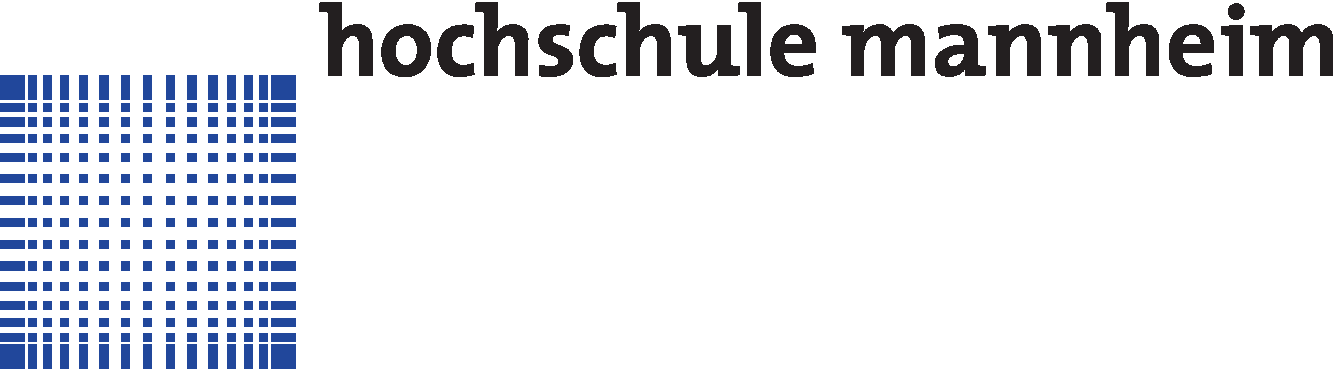
\includegraphics[width=7cm]{hsma-logo.pdf}\\

% Titel der Arbeit
\begin{textblock*}{128mm}(45mm,\seitenanfang + 62mm) % 4,5cm vom linken Rand und 6,0cm vom oberen Rand
  \centering\Large\sffamily
  \vspace{4mm} % Kleiner zusätzlicher Abstand oben für bessere Optik
  \textbf{\hsmatitel}
\end{textblock*}%

% Name
\begin{textblock*}{128mm}(45mm,\seitenanfang + 103mm)
  \centering\large\sffamily
  \hsmaautor
\end{textblock*}

% Thesis
\begin{textblock*}{\seitenbreite}(\bindekorrektur,\seitenanfang + 130mm)
  \centering\large\sffamily
  \hsmatyp\\
  \begin{small}\hsmathesistype \end{small}\\
  \vspace{2mm}
  \hsmastudiengangname
\end{textblock*}

% Fakultät
\begin{textblock*}{\seitenbreite}(\bindekorrektur,\seitenanfang + 165mm)
  \centering\large\sffamily
  \hsmafakultaetlang\\
  \vspace{2mm}
  \hsmakoerperschaft
\end{textblock*}

% Datum
\begin{textblock*}{\seitenbreite}(\bindekorrektur,\seitenanfang + 190mm)
  \centering\large 
  \textsf{\hsmadatum}
\end{textblock*}

% Firma
\begin{textblock*}{\seitenbreite}(\bindekorrektur,\seitenanfang + 215mm)
  \centering\large 
  %\textsf{Durchgeführt bei der Firma \hsmafirma}
\end{textblock*}

% Betreuer
\begin{textblock*}{\seitenbreite}(\bindekorrektur,\seitenanfang + 240mm)
  \centering\large\sffamily
  \hsmatutor \\
  \vspace{2mm}
  \hsmabetreuer\\
  \vspace{2mm}
  \hsmazweitkorrektor
\end{textblock*}

% Bibliographische Informationen
\null\newpage
\thispagestyle{empty}
  
\newcommand{\hsmabibde}{\begin{small}\textbf{\hsmaautorbib}: \\ \hsmatitelde \ / \hsmaautor. \ -- \\ \hsmatyp, \hsmaort \ : \hsmakoerperschaftde, \hsmajahr. \pageref{lastpage} Seiten.\end{small}}

\newcommand{\hsmabiben}{\begin{small}\textbf{\hsmaautorbib}: \\ \hsmatitelen \ / \hsmaautor. \ -- \\ \hsmatyp, \hsmaort \ : \hsmakoerperschaften, \hsmajahr. \pageref{lastpage} pages. \end{small}}

\ifthenelse{\equal{\hsmasprache}{de}}%
  {\hsmabibde \\ \vspace{0.5cm} \\ \hsmabiben}
  {\hsmabiben \\ \vspace{0.5cm} \\ \hsmabibde}


% Erklärung
\clearpage\setcounter{page}{1}
\thispagestyle{empty}
\textsf{\large\textbf{Erklärung}}

Hiermit erkläre ich, dass ich die vorliegende Arbeit selbstständig verfasst und keine anderen als die angegebenen Quellen und Hilfsmittel benutzt habe.

\ifthenelse{\boolean{hsmapublizieren} \and \not\boolean{hsmasperrvermerk}}%
{
\vspace{0.5cm}
Ich bin damit einverstanden, dass meine Arbeit veröffentlicht wird, d.\,h. dass die Arbeit elektronisch gespeichert, in andere Formate konvertiert, auf den Servern der Hochschule Mannheim öffentlich zugänglich gemacht und über das Internet verbreitet werden darf. 
}{}%

\vspace{1cm}
\hsmaort, \hsmadatum \\

\vspace{1.2cm}						                                      
\hsmaautor

\ifthenelse{\boolean{hsmasperrvermerk}}%
{%
\vspace{11cm}
\color{red}\textsf{\large\textbf{Sperrvermerk}}

Diese Arbeit basiert auf internen und vertraulichen Daten des Unternehmens \hsmafirma.

Diese Arbeit darf Dritten, mit Ausnahme der betreuenden Dozenten und befugten Mitglieder des Prüfungsausschusses, ohne ausdrückliche Zustimmung des Unternehmens und des Verfassers nicht zugänglich gemacht werden.

Eine Vervielfältigung und Veröffentlichung der Arbeit ohne ausdrückliche Genehmigung -- auch in Auszügen -- ist nicht erlaubt.
}{}

\cleardoublepage

% Abstract
\chapter*{Abstract}

\ifthenelse{\equal{\hsmasprache}{de}}%
  {\subsubsection*{\hsmatitelde}\hsmaabstractde\subsubsection*{\hsmatitelen}\hsmaabstracten}
  {\subsubsection*{\hsmatitelen}\hsmaabstracten\subsubsection*{\hsmatitelde}\hsmaabstractde}


% Inhaltsverzeichnis erzeugen
\tableofcontents

% Korrigiert Nummerierung bei mehrseitigem Inhaltsverzeichnis
\cleardoublepage
\newcounter{frontmatterpage}
\setcounter{frontmatterpage}{\value{page}}

% Arabische Zahlen für den Hauptteil
\mainmatter

% Den Hauptteil mit vergrößertem Zeilenabstand setzen
\onehalfspacing

% ------------------------------------------------------------------
% Hauptteil der Arbeit

\chapter{Einleitung}
\label{ch:einleitung}
\section{Das Projekt \sysplace}
\label{sec:sysplace}
Diese Master-Thesis wird im Rahmen des Projektes \sysplace (BMBF-gefördert, Förderkennzeichen 01IS14018D) verfasst. Das allgemeine Projektziel ist es, softwareentwickelnde \ac{KMU} in die Lage zu versetzen,
geräteübergreifende Systeme zu entwickeln, die neben einem bestmöglichen Nutzererlebnis eine hohe Kosten- / Nutzen Relation für \ac{KMU} ermöglichen. Hierfür sollen systematische Anleitungen zur Interaktionsgestaltung und Implementierung in Form von Entwurfs- und Entwicklungsansätzen, Guidelines und wiederverwendbaren Software-Komponenten entwickelt und validiert werden.

Drei zentrale Forschungsfragen wurden für das Projekt formuliert:
\begin{enumerate}
\item Wie lassen sich die Stärken der natürlichen Interaktion durch die Konzeption geeigneter Gesten auf das Gebiet der Ecosystems of Displays übertragen?
\item Welche methodisch-technischen Voraussetzungen sind notwendig, um diese Interaktionen zu unterstützen?
\item Welche Entwicklungsverfahren, -werkzeuge und -modelle und Voraussetzungen
muss die zugrunde liegende Softwarearchitektur des Gesamtsystems mitbringen, um
die Szenarien zu unterstützen?
\end{enumerate}

Die Erkenntnisse dieser Arbeit sollen vor allem einen Beitrag zur Beantwortung der letzten beiden Fragen liefern und basieren auf bereits erarbeiteten Forschungsergebnissen, die im folgenden Kapitel noch näher erläutert werden.

\section{Motivation und Zielsetzung}
Die meisten Menschen verbringen einen Großteil ihres Tages vor Bildschirmen verschiedenster Art, von Smartphones über Tablets zu Desktop-Rechnern und internetfähigen Fernsehern. Verschiedene Interaktionskonzepte sind entstanden, um diese Geräteübergänge für den Anwender intuitiv nutzbar zu machen. Aufgrund der heterogenen Darstellung und Umsetzung von Multiscreen-Konzepten werden diese im Forschungsprojekt SysPlace strukturiert und kategorisiert in Form von Interaktionsmustern erfasst und Designern sowie Entwicklern zur Verfügung gestellt. Aufgrund der hohen technischen Komplexität dieser Interaktionskonzepte fehlt bisher die Möglichkeit, die Details zur technischen Realisierung strukturiert und einheitlich in die Beschreibungen der Interaktionsmuster aufzunehmen.

Ziel dieser Arbeit ist es, die technischen Aspekte der verschiedenen Interaktionsmuster zu analysieren und eine formale Basis zu entwickeln, um diese einheitlich, abstrakt und plattformunabhängig beschreiben zu können. Dabei liegt der besondere Fokus auf der flexiblen Gestaltungsmöglichkeit von Interaktionsdetails.

Einzelne Interaktionskonzepte wurden hinsichtlich ihrer technischen Machbarkeit bereits von verschiedenen Institutionen und Forschern intensiv wissenschaftlich untersucht und prototypisch umgesetzt, zumeist mit einer an eine bestimmte Technologie gekoppelten Lösung. Zusammen mit den bereits im Projekt SysPlace konzipierten Prototypen bilden diese Vorarbeiten eine breite Basis, um daraus allgemeine Regeln für die Implementierung von Interaktionen im Multiscreen-Kontext abzuleiten.

Das Ergebnis der Arbeit ist ein Modell, das eine abstrakte, einheitliche Beschreibung der technischen Realisierung verschiedener Interaktionsmuster ermöglicht. Es soll Entwicklern die Möglichkeit bieten, die erforderlichen Komponenten, Abläufe und Nutzerinteraktionen sowie deren semantischen Zusammenhänge zu verstehen und konkret umsetzen zu können. Um das zu erreichen, wird die Modellbeschreibung so gestaltet, dass sie sich einfach in ausführbare Komponenten übersetzen lässt. 

Im Fokus der Arbeit steht dabei nicht, ein fertiges Framework zu entwickeln oder einzelne Interaktionsmuster mit konkreten Technologien zu realisieren. Zudem wird keine Bewertung vorgenommen, inwieweit sich einzelne Technologien zur Umsetzung bestimmter Aspekte von Interaktionsmustern eignen.

\section{Methodik}
Das Thema wird theoretisch auf Basis einer vergleichenden Literaturrecherche bearbeitet. Es werden Publikationen betrachtet, in denen geräteübergreifende Interaktionen theoretisch entworfen und anhand prototypischer Systeme evaluiert wurden. Den Ausgangspunkt bildet die Literatur, die bereits bei der Erfassung der Patterns im Projekt SysPlace betrachtet wurde. Es werden allerdings auch weitere Publikationen in die Recherche einbezogen, die den gleichen Forschungsgegenstand haben.

Das Ziel ist es, Gemeinsamkeiten und Unterschiede zwischen den verschiedenen Ansätzen zu analysieren und eine Abstraktion herauszuarbeiten, mit denen die heterogenen Konzepte geräteübergreifender Interaktionen einheitlich erfasst werden können. Das Ergebnis soll ein Modell sein, mit dem die technischen Realisierungsmöglichkeiten der analysierten Systeme sowie weiterer Systeme im Multiscreen-Kontext einheitlich beschrieben werden können. 

Zur Validierung der Ergebnisse werden einige Patterns anschließend exemplarisch durch das Modell beschrieben. Darauf aufbauend wird diskutiert, inwieweit sich die bisher erfassten Patterns durch das Modell beschreiben lassen, bzw. ob eine Erweiterbarkeit um neue Patterns gegeben ist.

\section{Aufbau}
Die Einleitung in diesem Kapitel stellt das Projekt vor, in dessen Rahmen diese Arbeit verfasst wurde und beschreibt anschließend die Motivation und Zielsetzung sowie die Methodik, die zum Erreichen des Ziels angewendet wird. Im zweiten Kapitel werden technische und konzeptionelle Grundlagen geräteübergreifender Interaktion beschrieben, die zum Verständnis der im Hauptkapitel analysierten Literatur relevant sind. Kapitel \ref{ch:modell} beinhaltet eine ausführliche Analyse geräteübergreifender Interaktionen und bildet somit den eigenen Beitrag der Arbeit, indem ein Modell erarbeitet wird, das die in der Einleitung vorgestellte Problemstellung löst. Eine Validierung der Ergebnisse wird in Kapitel \ref{ch:validierung} entsprechend der beschriebenen Methodik vorgenommen. Abschließend wird eine Zusammenfassung der erarbeiteten Ergebnisse sowie ein Überblick über mögliche weiterführende in Kapitel \ref{ch:zusammenfassung} gegeben.

\chapter{Technische und konzeptionelle Grundlagen}
\label{ch:grundlagen}
In diesem Kapitel werden technische Grundlagen und Begriffsdefinitionen behandelt, die für das Verständnis der Arbeit relevant sind. Auf konzeptioneller Ebene werden zunächst zentrale Begriffe und deren Verwendung innerhalb der Arbeit definiert. Anschließend wird ein Überblick über Zweck und Verwendung von Entwurfsmustern bei der Oberflächen- und Interaktionsgestaltung gegeben. 

Auf der technischen Ebene wird zunächst das Spektrum vorhandener Gerätetypen für Multiscreen-Szenarien vorgestellt, klassifiziert und eingeschränkt. Anschließend werden Technologien beschrieben, die besonders geeignet für die Realisierung von Multiscreen-Anwendungen sind. Da ein Gesamtüberblick unmöglich ist, wird hier eine Auswahl von verbreiteten und aktuell verfügbaren Technologien vorgenommen.

\section{Multiscreen}
\label{sec:multiscreen}
Das zentrale Thema dieser Arbeit ist die Gestaltung von Interaktionen, die den Nutzer in die Lage versetzen, eine zusammenhängende Aufgabe geräteübergreifend auf mehreren Displays zu erledigen.

Ein häufig in der Literatur zu findender Begriff ist der des \textit{\ac{MDE}}, der von Seyed \ua wie folgt definiert wird \citep{Seyed2012}:
\begin{quote}
A multi-display environment (MDE) is a system where
interaction is divided over several displays, such as digital
tabletops, wall displays and personal devices like tablets or
mobile phones. MDEs often include heterogeneous displays
to take advantage of different capabilities such as their size,
position, resolution or mobility to support the task at hand.
\end{quote}

Der Begriff \ac{MDE} ist in der Fachliteratur seit gut einer Dekade zu finden und wird bereits von \cite{Rekimoto1997} für die Kombination mehrerer Geräte wie Desktop-PCs, \acp{PDA} und größeren Wandbildschirmen verwendet.

Um den interaktiven Aspekt bei der gemeinsamen Nutzung verschiedener Geräte noch mehr hervorzuheben, sprechen Terrenghi und Kollegen von einem \textit{ecosystem of displays}, das an den jeweiligen Nutzungskontext angepasst werden kann \citep{Terrenghi2009}. 

Mit \textit{symphony of devices} definieren Hamilton und Kollegen einen weiteren Begriff, der bewusst gewählt wurde, um eine Ad-hoc-Kombination heterogener Geräte, je nach Anwendungsfall, in den Vordergrund zu stellen. Zudem soll dadurch eine Abgrenzung zu anderer Forschung stattfinden, in der dieser Aspekt nicht explizit beleuchtet wird \citep{Hamilton2014}.

Diese Arbeit folgt einer Definition von Nagel und Fischer. Diese verwenden die Begriffe \textit{device} und \textit{screen} (und damit auch \textit{display}) synonym für digitale Endgeräte \citep[16]{Nagel2013}. Mittels solcher Endgeräte können Informationen abgerufen, dargestellt und bearbeitet werden. Der Bildschirm eines Gerätes ist ausschlaggebend für die Art und Repräsentation der Informationen, die abgerufen werden können. Zudem ist bei mobilen Endgeräten der Bildschirm zumeist fest verbaut und bildet damit eine Einheit mit dem eigentlichen Gerät, weshalb diese Gleichsetzung der Begriffe \textit{device} und \textit{screen} sinnvoll ist.

Darauf aufbauend wird für die Kombination mehrerer Geräte in einem gemeinsamen Nutzungskontext der Begriff \textit{Multiscreen}, im Singular zumeist die Begriffe Gerät und Endgerät verwendet \citep{Nagel2013}. Auch bei Google findet sich der Begriff Multiscreen in einer umfangreichen Studie, die die Nutzung verschiedener Geräte wie Smartphones, Tablets und PCs zur Erledigung zusammenhängender Aufgaben analysiert \citep{Google2012}. Damit bezeichnet Multiscreen nicht nur einen Rechner mit mehreren Monitoren, sondern die Kombination verschiedener heterogener Endgeräte.

Darüber hinaus werden in dieser Arbeit die folgenden Begriffe verwendet:
\begin{itemize}
\item \textit{(End)gerät}: Ein einzelnes Gerät (\zb Desktop-PC, Tablet etc.), das in einem Multiscreen-Szenario verwendet werden kann.
\item \textit{Multiscreen-Szenario}: Ein Anwendungsfall, in dem verschiedene (heterogene) Geräte zur Erledigung einer zusammenhängenden Aufgabe genutzt werden \citep[19]{Nagel2013}.
\item \textit{Multiscreen-Anwendung}: Eine Anwendung, die auf verschiedenen Endgeräten nutzbar ist und Daten geräteübergreifend bereitstellen kann \citep[18]{Nagel2013}. Eine Multiscreen"=Anwendung kann ein Multiscreen"=Szenario teilweise oder ganz realisieren.
\item \textit{Multiscreen-Interaktion}: Interaktionen, die dem Nutzer ermöglichen, geräteübergreifend zu arbeiten (\zb Verbinden von Geräten, Datenübertragung etc.); Begriffsprägung analog zu Multiscreen-Szenario und -Anwendung.
\item \textit{Multiscreen-Pattern}: Ein Entwurfsmuster, das die Gestaltung und Implementierung von Multiscreen-Interaktionen unterstützen soll; begriffliche Einordnung der Patterns in den Multiscreen-Kontext.
\end{itemize}

Zudem unterscheidet Google zwei Modi für die Multiscreen-Nutzung \citep{Google2012}:
\begin{itemize}
\item \textit{Sequentielle Nutzung}: der Nutzer wechselt während einer zusammenhängenden Aktivität von einem Gerät zum anderen.
\item \textit{Simultane Nutzung}: der Nutzer verwendet zwei Geräte parallel für zusammenhängende oder unzusammenhängende Aktivitäten.
\end{itemize}

Im folgenden Kapitel werden Geräte, die für Multiscreen-Szenarien in Frage kommen, näher erläutert und in Klassen eingeteilt, sodass sie im weiteren Verlauf der Arbeit eindeutig referenziert werden können. 

\section{Geräteklassen für Multiscreen-Interaktionen}
\label{sec:geräteklassen}
Es existiert eine kaum überschaubare Anzahl verschiedenster Geräte, die in Multiscreen"=Szenarien einsetzbar sind. Dabei stehen klassische Desktop-PCs bzw. Laptops nicht mehr im Mittelpunkt, sondern machen nur noch etwa ein Viertel der täglichen Medieninteraktion aus und wurden bei der Nutzungshäufigkeit von Smartphones verdrängt \citep{Google2012}. Schon lange bevor Smartphones allgegenwärtig wurden, gab es mobile Geräte unter verschiedenen Bezeichnungen wie \ac{PDA}, PocketPC, Palm etc., deren Einsatzmöglichkeiten in Multiscreen"=Szenarien bereits früh erforscht wurden \citep{Hinckley2004}. 

Apple konnte 2010 mit der Einführung des iPad, das sich in weniger als drei Monaten mehr als 3 Millionen mal verkaufte, Tablets als zusätzliche Geräteklasse auf dem Markt etablieren \citep{Apple2010}. Tablets werden heute von vielen verschiedenen Herstellern angeboten und vorwiegend zur Unterhaltung und Kommunikation eingesetzt \citep{Google2012}. Die Bildschirmgröße und technische Ausstattung von Tablets können stark variieren.

Das klassische TV ist nach wie vor präsent, wird aber meist in Verbindung mit einem anderen Gerät simultan benutzt \citep{Google2012} und ist eher ein "`Hintergrundrauschen"' \citep{Microsoft2013}.

Google unterscheidet in seiner Studie zwischen vier verschiedenen Geräteklassen sowie üblichen Nutzungsszenarien und -orten \citep{Google2012}:
\begin{enumerate}
\item \textit{Smartphone}: Zu Hause oder unterwegs für Kommunikation und schnelle Informationsbeschaffung.
\item \textit{Tablet}: Überwiegend zur Unterhaltung zu Hause.
\item \textit{PC/Laptop}: Produktives, konzentriertes Arbeiten zu Hause oder im Büro.
\item \textit{TV}: Zu Hause zur Unterhaltung, oft parallel mit Geräten anderer Klassen.
\end{enumerate}

\begin{figure}
\centering
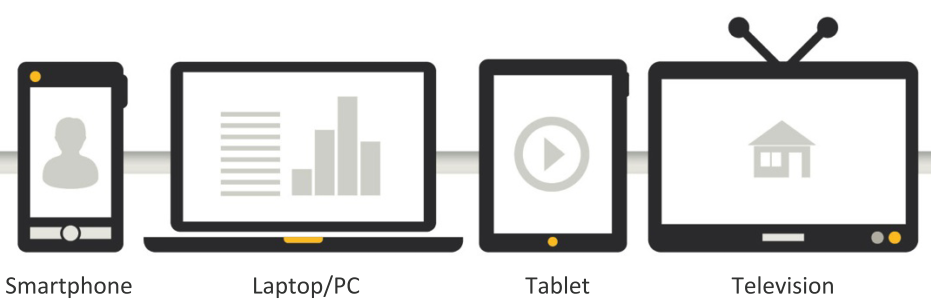
\includegraphics[width=\textwidth]{bilder/4_devices.png}
\caption{Die vier Geräteklassen Smartphone, PC/Laptop, Tablet, (Smart) TV. Quelle: \citep{Google2012}.}
\end{figure}
Microsoft hat dieselben vier Kategorien und sehr ähnliche Nutzungskontexte herausgearbeitet \citep{Microsoft2013}. Auch bei Nagel und Fischer werden diese Kategorien unter der Bezeichnung "`Vier Screens"' genannt, eine interessante Ergänzung im Hinblick auf Multiscreen-Interaktion ist hier allerdings die Einschränkung der Kategorie TV auf internetfähige Geräte, sog. \textit{Smart TVs} \citep[31]{Nagel2013}. Erst durch die Vernetzung mit anderen Geräten können TV-Geräte in Multiscreen-Szenarien wirklich sinnvoll verwendet werden. 

\begin{figure}
\centering
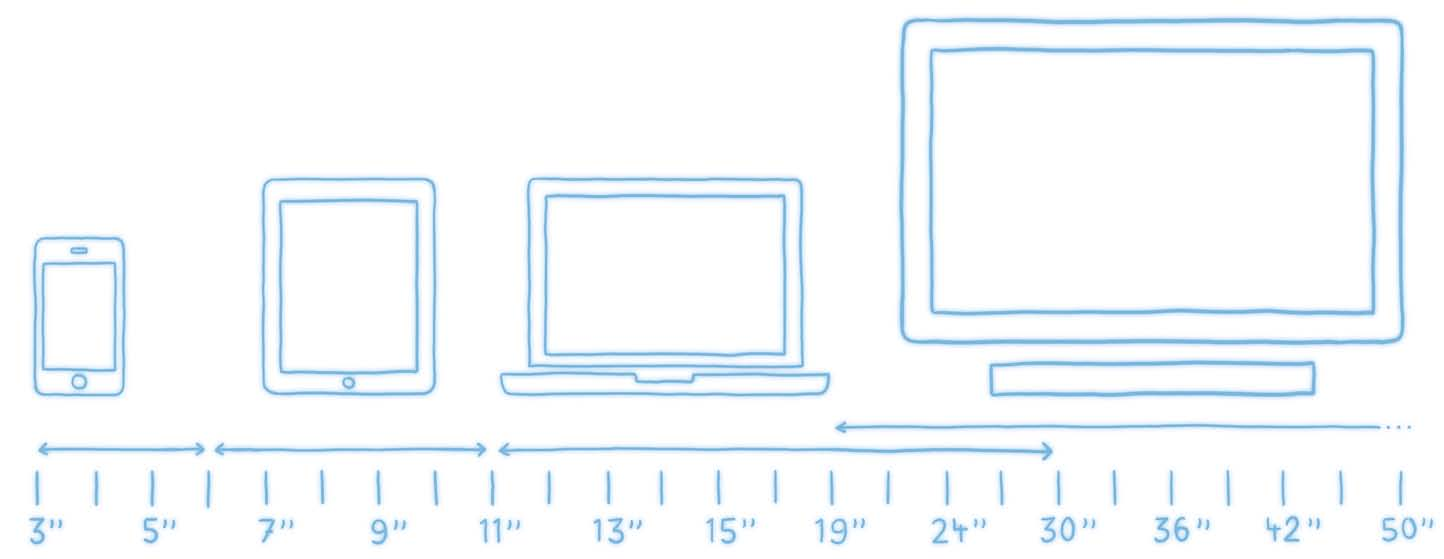
\includegraphics[width=\textwidth]{bilder/devices.png}
\caption{Die vier Geräteklassen und deren übliche Screengröße in Relation. Quelle: \citep{Nagel2013}.}
\end{figure}

Zwei Ergänzungen zu diesen vier Kategorien werden für diese Arbeit vorgenommen. Auf der einen Seite sind für Multiscreen-Szenarien auch größere Displays als Smart TVs denkbar. So ermöglicht \zb das System "`Dynamo"' das Teilen von Daten über ein öffentlich nutzbares Display, das eine gesamte Wand einnimmt \citep{Izadi2003}. Um solche Displays für Multiscreen-Anwendungen nutzbar zu machen, müssen sie netzwerkfähig sein, weshalb sie einfach zu den Smart TVs gezählt werden können.

Auf der anderen Seite stehen Geräte wie Fitnesstracker, Datenbrillen oder mit Sensoren versehene Kleidungsstücke, die direkt am Körper getragen werden. Diese Geräte werden oft als \textit{Wearables} bezeichnet. Im Rahmen dieser Arbeit wird diese Kategorie ausgeklammert, da die Interaktion mit solchen Geräten entweder sehr komplex ist, wie \zb bei \ac{AR}- und \ac{VR}-Brillen, oder aufgrund weniger Sensoren kaum explizit möglich ist, wie \zb \cite{Yoon2014} feststellt.

Lediglich sog. \textit{Smartwatches}, die seit dem Erscheinen der Pebble im Jahr 2012 als alleinstehende oder ergänzende Geräte zu Tablets oder Smartphones große Verbreitung finden\footnote{Prognosen gehen davon aus, dass der Markt für Smartwatches bis 2018 auf 214 Millionen Stück wachsen wird \citep{Rawassizadeh2014}.}, könnten in Multiscreen-Szenarien zum Einsatz kommen. Die Voraussetzung ist, dass sie programmierbar sind und dem Anwender explizite Interaktionsmöglichkeiten bieten. Da die Anwendungsfälle bzgl. Multiscreen-Interaktionen denen von Smartphones ähneln, werden Smartwatches in dieser Arbeit nicht gesondert betrachtet. Für Smartphones, Tablets und Smartwatches wird der Sammelbegriff \textit{mobile Geräte} verwendet.

Weil diese Arbeit auf einer Sammlung von Entwurfsmustern zur Multiscreen"=Interaktion aufbaut, wird im nächsten Kapitel der Begriff des Patterns definiert und in Bezug zu Multiscreen-Interaktionen gesetzt.

\section{Multiscreen-Patterns}
\label{sec:msp-patterns}
Entwurfsmuster (engl. \textit{design patterns}) haben ihren Ursprung in der Architektur und werden durch das folgende, obligatorische Zitat von Alexander präzise und allgemeingültig definiert \citep{Alexander1977}: 
\begin{quote}
Each pattern describes a problem which occurs over and over again in our environment, and then describes the core of the solution to that problem, in such a way that you can use this solution a million times over, without ever doing it the same way twice.
\end{quote}
Auch -- oder gerade besonders -- in der Informatik gibt es viele wiederkehrende Probleme, für deren Lösung Patterns hilfreich sein können. Die erste und wohl bekannteste Patternsammlung, die im Bereich der Informatik von Gamma und Kollegen veröffentlicht wurde, behandelt eine Vielzahl von Problemstellungen der objektorientierten Programmierung \citep{Gamma1995}.
Speziell im Bereich der GUI- und Interaktionsgestaltung gibt es verschiedene Patternsammlungen, wobei die von \cite{Yahoo2015}, \cite{Tidwell2010} und \cite{Welie2008} zu den bekanntesten gehören. Während Yahoo überwiegend typische Webdesignprobleme wie Tabs, Fortschrittsbalken und Autovervollständigung adressiert, finden sich bei Tidwell und van Welie \zb auch Patterns zum Designkontext (Nutzererwartungen an die Webseite, verschiedene Seitentypen etc.) oder der Visualisierung von Daten.

Alle Patternsammlungen haben die Gemeinsamkeit, dass die Patterns in einer jeweils konsistenten, strukturierten Form erfasst werden. Das hat den Vorteil, dass Patterns einfacher zu lernen, zu vergleichen und anzuwenden sind \citep[6]{Gamma1995}. Die konkrete Struktur variiert zwischen den einzelnen Patternsammlungen, folgende Bestandteile sind aber meist vorhanden:
\begin{itemize}
\item \textit{Eindeutiger Name}: Wie lässt sich das Pattern prägnant nennen? Hilfreich für die eindeutige Referenzierung von Patterns.
\item \textit{Problembeschreibung}: Welches Problem löst das Pattern?
\item \textit{Lösung}: Welche Schritte sind notwendig, um das Problem zu lösen? Je nach Domäne des Patterns ergänzt um konkrete Lösungshinweise, wie \zb Code-Beispiele.
\item \textit{Wann}: In welchem Kontext kann das Pattern eingesetzt werden, in welchem eher nicht?
\item \textit{Warum}: Aus welchen Gründen ist das Pattern zur Lösung des Problems geeignet?
\item \textit{Bekannte Anwendungen}: Wo wurde das Pattern bereits erfolgreich eingesetzt?
\end{itemize}

Die Patternsammlung, die im Projekt \sysplace erarbeitet wird, folgt einer analogen Struktur. Jedes Pattern wird mittels eines \textit{Templates} erfasst. Ein ausgefülltes Template ist exemplarisch in Anhang \ref{a:patterntemplate} zu finden. Da Multiscreen-Interaktionen mit verschiedenen Gerätekombination und in vielfältigen Anwendungskontexten stattfinden können, wird in den Punkten "`Wann"' (geeignete Nutzungskontexte) und "`Warum"' (Begründung der Intuitivität der Interaktion) dargelegt, warum das Pattern in bestimmten Situationen eine geeignete Multiscreen-Interaktion realisiert. Zur weiteren Strukturierung ist die Patternsammlung in fünf Kategorien unterteilt:
\begin{itemize}
\item \textit{Give}: Daten an ein anderes Gerät senden.
\item \textit{Take}: Daten von einem anderen Gerät empfangen.
\item \textit{Exchange}: Dateien zwischen zwei Geräten austauschen / synchronisieren.
\item \textit{Extend}: Mehrere Bildschirme koppeln.
\item \textit{Connect}: Zwei Geräte miteinander verbinden.
\end{itemize}

Der Name jedes Patterns folgt dem Namensschema \textit{<Verb> To <Kategorie>}, also \zb \textit{Bump To Exchange} oder \textit{Swipe To Give}. Das Verb beschreibt möglichst prägnant die zugrunde liegende \textit{Geste}\footnote{Der Begriff Geste wird hier analog zu Echtler im weitest möglichen Sinne gebraucht, also als Reaktion eines Systems auf eine Untermenge aller möglichen Nutzereingaben (Multitouch, Handbewegungen, Eingaben mit einem digitalen Stift etc.)  \citep{Echtler2012}.} des Patterns, die Kategorie definiert die Art der angestoßenen Systemreaktion. Das Pattern "`Swipe To Give"' bezeichnet demnach eine Wisch-Geste des Nutzers, die die Übertragung einer Datei von einem Gerät auf ein anderes anstößt. In Anhang \ref{a:patterns_all} ist eine Zusammenfassung aller Patterns zu finden.

Die zentrale Problemstellung, die in dieser Arbeit bearbeitet wird, ist innerhalb des Templates unter dem Punkt "`Technisches"' bei der Beschreibung des Lösungsansatzes verortet, bezieht aber auch weitere Aspekte mit ein.

\section{Relevante Technologien}
Multiscreen-Anwendungen realisieren Interaktionskonzepte, die vielfältige Anforderungen an die Hard- und Software der verwendeten Geräte stellen. Neben der Konnektivität spielen sowohl Sensoren (zur Messung von Geräteeingaben verschiedener Art) als auch Ausgabetechnologien eine entscheidende Rolle.
In den folgenden Unterkapiteln werden die wichtigsten Technologien vorgestellt und deren Einsatzmöglichkeiten aufgezeigt.

\subsection{Konnektivität}
\label{subsec:connectivity}
\subsubsection{Ethernet und WLAN}
Die am weitesten verbreitete Technologie zum Verbinden von Geräten ist Ethernet\footnote{Oft synonym verwendet mit \ac{LAN} oder Ethernet-LAN.}, wobei heute zumeist der Protokollstandard IEEE 802.3 oder Abwandlungen davon eingesetzt werden. Ethernet ist kabelgebunden und erreicht in heute gängigen Standards üblicherweise eine Übertragungsgeschwindigkeit von \SI{100}{\mega\Bit\per\second} bis \SI{10}{\giga\Bit\per\second} auf Distanzen von 100 Metern (Kupferkabel) bis zu mehreren Kilometern (Glasfaserkabel) \citep[506-507]{Kurose2014}. In Multiscreen-Szenarien ist Ethernet allerdings nur eingeschränkt für Geräte der Kategorie PC/Laptop oder Smart TV einsetzbar, aber nicht für mobile Geräte.

Unter dem Begriff \ac{WLAN}\footnote{Oft synonym mit Wi-Fi verwendet.} haben sich Funknetzwerke als Alternative zum kabelgebundenen Ethernet durchgesetzt. Obwohl der Begriff \ac{WLAN} für viele Arten von Funknetzwerken verwendet wird, ist damit meist ein Standard der Normenfamilie IEEE 802.11 gemeint. Die Übertragungsgeschwindigkeit ist oft niedriger als bei Ethernet-Netzwerken, wobei neuere Standards inzwischen auch in den \si{\giga\Bit}-Bereich vordringen. Mit den gängigen Standards (vgl. Tabelle \ref{tab:wlan}) lassen sich Distanzen von ca. 10 -- 30 m überbrücken \citep[552]{Kurose2014}.

\begin{table}[h]
\centering
\ra{1.3}
\begin{tabular}{lll@{}}\toprule
Standard & Frequenzbereich (USA) & Übertragungsrate \\ 
\midrule
802.11b & \(2.4\) -- \(\SI{2.485}{\giga\hertz}\) & bis \(\SI{11}{\mega\Bit\per\second}\) \\ 
802.11a & \(5.1\) -- \(\SI{5.8}{\giga\hertz}\) & bis \(\SI{54}{\mega\Bit\per\second}\) \\ 
802.11g & \(2.4\) -- \(\SI{2.485}{\giga\hertz}\) & bis \(\SI{54}{\mega\Bit\per\second}\) \\ 
\bottomrule
\end{tabular} 
\caption{Gängige WLAN-Standards. Quelle: \citep[562]{Kurose2014}.}
\label{tab:wlan}
\end{table}

\begin{figure}[h]
\centering
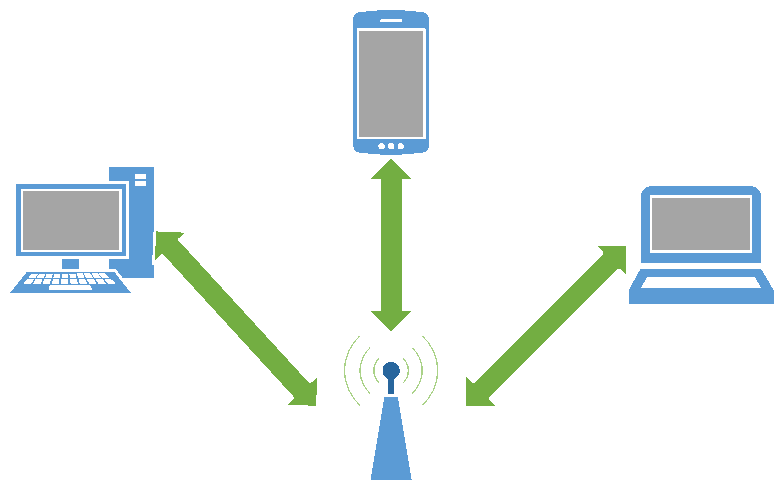
\includegraphics[width=0.7\textwidth]{bilder/infrastruktur_modus}
\caption{\ac{WLAN} im Infrastrukturmodus.}
\label{fig:infrastructure_mode}
\end{figure}

Drahtlose Netzwerke können in zwei Modi betrieben werden \citep[555]{Kurose2014}:
\begin{itemize}
\item \textit{Infrastruktur-Modus}: Alle Geräte im Netzwerk kommunizieren mit einer Basisstation, die wiederum mit weiteren Netzwerken oder dem Internet verbunden sein kann (siehe Abbildung \ref{fig:infrastructure_mode}).
\item \textit{Ad-hoc-Modus}: Es gibt keine Basisstation, alle Geräte kommunizieren direkt miteinander (siehe Abbildung \ref{fig:adhoc_mode}).
\end{itemize}

Für beide Modi gibt es in Multiscreen"=Szenarien Anwendungsmöglichkeiten. Die meisten mobilen Geräte sowie PCs und Laptops verfügen über einen WLAN"=Adapter. Im Infrastruktur-Modus können Geräte aller Kategorien über die Basisstation miteinander kommunizieren, entweder direkt per \ac{WLAN} oder durch an die Basisstation angeschlossene Geräte wie \zb Smart TVs, die nur eine Ethernet-Schnittstelle besitzen. Um ganz auf die Basisstation zu verzichten, können Multiscreen"=Anwendungen auch den Ad"=hoc"=Modus nutzen. Das hat den Vorteil, dass Geräte auch ohne Anmeldung an einer Basisstation miteinander verbunden werden können. Damit entfällt die Notwendigkeit, für Multiscreen-Anwendungen eine feste Netzwerkinfrastruktur einzurichten.

\begin{figure}[h]
\centering
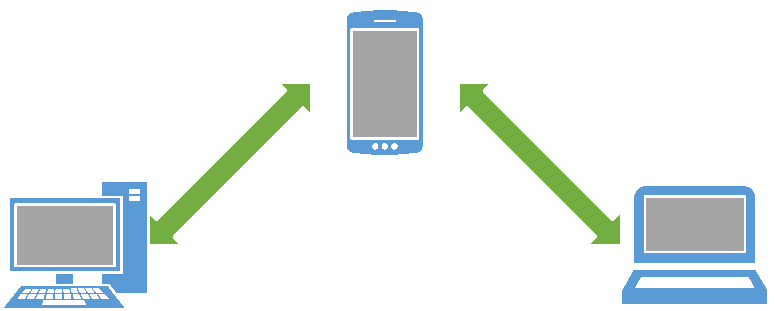
\includegraphics[width=0.7\textwidth]{bilder/ad_hoc_modus}
\caption{\ac{WLAN} im Ad-Hoc-Modus.}
\label{fig:adhoc_mode}
\end{figure}

Mit Wi-Fi Direct wird im nächsten Kapitel ein Standard vorgestellt, der es ermöglicht, den Ad-hoc-Modus relativ einfach universell einzusetzen.

\subsubsection{Wi-Fi Direct}
Wi-Fi Direct ist ein von der Wi-Fi Alliance\footnote{Die Wi-Fi Alliance ist eine 1999 gegründete Non-Profit-Organisation mit dem Ziel, her\-stel\-ler\-un\-ab\-häng\-ige Standards für die drahtlose Kommunikation zu spezifizieren und deren Einhaltung zu zertifizieren \citep{WifiAllianceAbout}.} spezifizierter Standard zur direkten, drahtlosen Verbindung von Geräten basierend auf den IEEE 802.11 Netzwerkstandards. Mit Wi-Fi Direct ist es möglich, zwei Geräte direkt oder mehrere Geräte als Gruppe miteinander zu verbinden, um \zb Dateien auszutauschen, Geräte zu synchronisieren oder Drucker anzusteuern \citep{WifiDirect}. 

Ebenso ermöglicht Wi-Fi Direct, Geräte in der Nähe zu finden und die eigentliche Übertragung von Daten durchzuführen. Eine Basisstation oder Internetverbindung ist nicht nötig, es wird also ein Ad-hoc-Modus realisiert, bei dem ein Wi-Fi Direct fähiges Gerät die Verantwortung für die Gruppenkoordination übernehmen kann \citep{WifiDirect}.

Für den Einsatz in Multiscreen-Anwendungen spricht, dass Wi-Fi Direct her\-stel\-ler\-un\-ab\-hän\-gig ist und über System-\acsp{API} auf einer Vielzahl vor allem mobiler Endgeräte einfach verwendet werden kann. Zudem können die hohen Übertragungsgeschwindigkeiten des jeweils zugrunde liegenden Drahtlosstandards genutzt werden, was den Austausch größerer Datenmengen ermöglicht, als es \zb bei Bluetooth oder NFC der Fall ist.

\subsubsection{Bluetooth}
\label{subsec:bluetooth}
Bluetooth ist ein weit verbreiteter Standard für eine drahtlose, verbrauchsarme Funktechnologie.
Die Spezifikation und Weiterentwicklung des Standards liegt in der Verantwortung der \ac{SIG}. Basierend auf einer 1994 von Ericsson durchgeführten Studie wurde Bluetooth mit dem Ziel entwickelt, drahtlose Datenübertragung im ISM-Band\footnote{Das \ac{ISM}-Band ist ein Frequenzbereich (2,4 bis 2,485 GHz), der ohne Lizenzkosten genutzt werden kann und daher universell verwendbar ist.} auf kurzen Distanzen zu realisieren \citep[121]{Fuchs2009}.

Aufgrund der niedrigen Hardwarekosten und dem fast ubiquitären Einsatz von Bluetooth kann eine Vielzahl von Geräten miteinander verbunden werden. Durch das sog. \textit{Pairing} werden zwei Geräte gekoppelt, um einen Verbindungsaufbau zwischen den Geräten zu ermöglichen. Bluetooth folgt dabei immer der Topologie eines \textit{Piconetzes}, in dem ein Gerät (Master) die Koordination von bis zu sieben aktiven Geräten (Slaves) übernimmt \citep[579]{Kurose2014}. Die Kommunikation erfolgt immer über den Master, wodurch sich ein sternförmiges Netz ergibt (siehe Abbildung \ref{fig:piconet}).

\begin{figure}[ht]
\centering
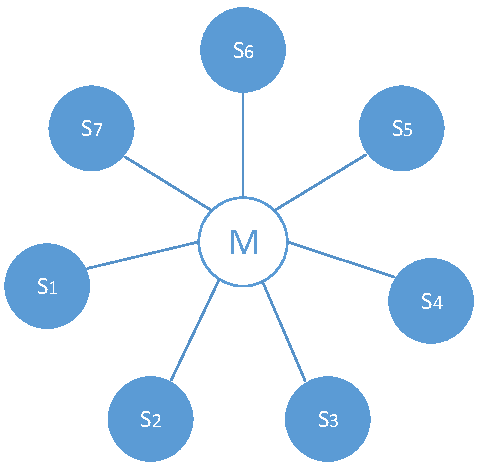
\includegraphics[width=0.4\textwidth]{bilder/piconet}
\caption{Piconetz aus einem Master und der Maximalzahl von sieben Slaves. Angelehnt an \citep[125]{Fuchs2009}.}
\label{fig:piconet}
\end{figure}

Eine wichtige Neuerung in der aktuellen Version 4.2 ist \ac{BLE}\footnote{Auch vermarktet als Bluetooth Smart.}. Das Bluetooth-Protokoll wurde komplett überarbeitet und der Stromverbrauch deutlich reduziert. Durch \ac{BLE} können so auch viele Geräte, die vorher aus Gründen der Stromersparnis proprietäre Funkstandards verwendet haben, über den universellen Bluetooth Standard miteinander kommunizieren \citep{Hansen2015}.

Der Bluetooth-Standard ist in verschiedenen Versionen verfügbar, in denen jeweils andere Features und Übertragungsbandbreiten spezifiziert sind. Die Versionen 4.0 und höher sind mit den vorigen nicht kompatibel, weshalb oft eine Unterscheidung zwischen \ac{BLE} und Bluetooth Classic vorgenommen wird, wobei mit Bluetooth Classic meist die Version 2.1 gemeint ist. Bluetooth Classic erreicht Geschwindigkeiten von ca. 700 KBit/s (Version 1.1) bis ca. 2 MBit/s (Version 2.1 + EDR) \citep[129]{Fuchs2009}.  

Die Übertragungsgeschwindigkeit von \acs{BLE} ist zwar mit \SI{1}{\mega\Bit\per\second} deutlich höher als \zb bei \acs{NFC} (siehe Kapitel \ref{subsec:nfc}), kann aber nicht mit Ethernet, WLAN oder Bluetooth Classic konkurrieren \citep{Wikipedia2015}. Allerdings basieren andere, für Multiscreen"=Szenarien interessante Protokolle auf \ac{BLE}, die im folgenden Kapitel vorgestellt werden.

\subsubsection{iBeacon und Eddystone}
\label{subsec:ibeacon}
Aufbauend auf \ac{BLE} spezifiziert Apple mit \textit{iBeacon} ein proprietäres Protokoll, das es ermöglicht, Distanzen zu anderen Geräten zu messen und diese eindeutig zu identifizieren. Mittels \ac{BLE} können auch kleine, batteriebetriebene Geräte kontinuierlich ein Bluetooth-Signal aussenden, das sog. \textit{Beacon} (deut. Signal- oder Leuchtfeuer). Die Nutzdaten dieses Signals werden im iBeacon-Protokoll so spezifiziert, dass sie einen eindeutigen \ac{UUID} sowie zwei weitere Werte, die Major- und Minor-Nummer, übermitteln können \citep{iBeacon}. Es muss kein Pairing der Geräte stattfinden, da alle notwendigen Informationen bereits in den sog. Advertisement-Paketen des BLE-Signals übermittelt werden.

Für ein sendendes Gerät werden zumeist die Begriffe iBeacon und Beacon synonym verwendet, wobei Beacon allgemeiner ist und auch andere Protokolle einschließt. 

\begin{figure}[ht]
\centering
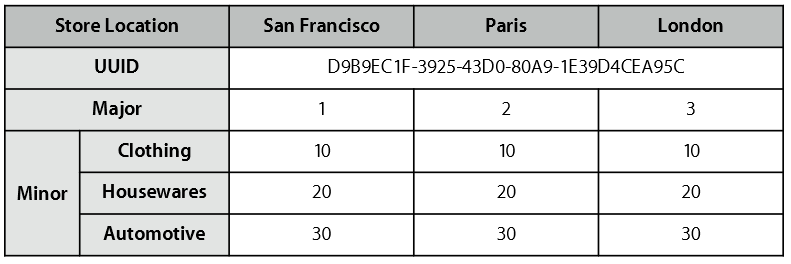
\includegraphics[scale=0.65]{bilder/ibeacon.png}
\caption{Nutzung von \acs{UUID}, Major- und Minor-Nummer zur Realisierung einer Lokalisierung mittels iBeacon. Quelle: \citep{iBeacon}.}
\label{fig:ibeacon}
\end{figure}

Abbildung \ref{fig:ibeacon} zeigt exemplarisch, wie mittels dieser Werte Abteilungen in verschiedenen Niederlassungen einer Kaufhauskette identifiziert werden könnten. Die \ac{UUID} ist weltweit eindeutig für die Organisation, während die Major- und Minor-Nummern für die Niederlassung bzw. die Art der Abteilung verwendet werden. So kann jedes Beacon individuell für den jeweiligen Anwendungsfall konfiguriert werden.

Neben diesen Werten kann ein empfangendes Gerät anhand der Stärke des \ac{BLE}-Signals den Abstand zu dem Beacon messen, wobei Apple vier verschiedene Abstände unterscheidet \citep{iBeacon}:
\begin{itemize}
\item \textit{Immediate}: Sehr naher, fast direkter Kontakt zwischen Beacon und Empfänger.
\item \textit{Near}: Abstand von ein bis drei Metern.
\item \textit{Far}: Abstand von mehr als drei Metern.
\item \textit{Unknown}: Der Abstand kann nicht zuverlässig ermittelt werden.
\end{itemize}
Physikalische Barrieren, ein schwaches \ac{BLE}-Signal oder hohe Last auf der verwendeten Bluetooth-Frequenz können die Genauigkeit der Abstandsmessung beeinträchtigen.

Google versucht mit \textit{Eddystone} ein offenes Protokoll zu etablieren, das das proprietäre iBeacon ablösen soll und Beacons semantisch wertvollere Daten senden lässt \citep{Eddystone}:
\begin{itemize}
\item \textit{Eddystone-UID}: Eine eindeutige ID analog zur UUID von iBeacon.
\item \textit{Eddystone-URL}: Eine kurze \acs{URL}, die vom Client verwendet werden kann.
\item \textit{Eddystone-TLM}: Ein Telemetriepaket zur Überwachung des Zustandes von Beacons.
\end{itemize}

Neben batteriebetriebenen Sendern ist es möglich, \zb Smartphones oder Tablets direkt als Beacons zu verwenden. Apple sieht darin zwar nur begrenzte Anwendungsmöglichkeiten \citep{iBeacon}, für Multiscreen"=Szenarien ist allerdings auch diese Variante denkbar.

\subsubsection{NFC}
\label{subsec:nfc}
\ac{NFC} ist ein seit 2002 entwickelter Standard zum drahtlosen Datenaustausch zwischen mobilen Endgeräten. Seit 2004 übernimmt das NFC Forum die Weiterentwicklung des Standards und bietet Informationen zur Entwicklung von NFC-fähiger Software an \citep{NFCAbout}. 

Im Gegensatz zu anderen Drahtlostechnologien wie WLAN oder Bluetooth funktioniert NFC nur in unmittelbarer Nähe der zu verbindenden Geräte (bis zu 20 cm). Dadurch kann der Anwender schon durch räumliche Distanz eine ungewollte Verbindung zu anderen Geräten verhindern. Der Standard ist mit der bereits weit verbreiteten \acs{RFID}-Technologie kompatibel und kann passive RFID-Tags im 13,56-MHz Band auslesen \citep[30]{Want2006}. Die Übertragungsgeschwindigkeit ist auf \SI{424}{\kilo\Bit\per\second} limitiert. 

NFC kann in drei verschiedenen Modi betrieben werden (siehe Abbildung \ref{fig:nfc_modes}). Im Tag-Reader/Writer-Modus ist es möglich, Tags auszulesen; so können physikalische Objekte mittels extern angebrachter Tags mit elektronisch auslesbaren Informationen versehen werden. Damit können \zb Fahrpläne um Echtzeitinformationen erweitert werden \citep{NFCWhat}.

Im Peer-to-Peer-Modus können Geräte direkt miteinander kommunizieren und Daten austauschen, allerdings ist die Bandbreite eine entscheidende Limitierung für die Art der auszutauschenden Daten. Im Card Emulation Modus kann sich ein NFC-fähiges Gerät als Smart Card ausgeben und in bestehende Smart Card Infrastrukturen integriert werden \citep{NFCWhat}. 

Vor allem die ersten beiden Modi sind für Multiscreen-Szenarien interessant, um Geräte zu verbinden, kleinere Datenmengen auszutauschen oder physikalische Objekte in Interaktionen mit einzubeziehen. Die meisten mobilen Geräte sind heute mit NFC ausgestattet, was den Einsatz besonders für diese Gerätekategorie attraktiv macht.

\begin{figure}
\begin{center}
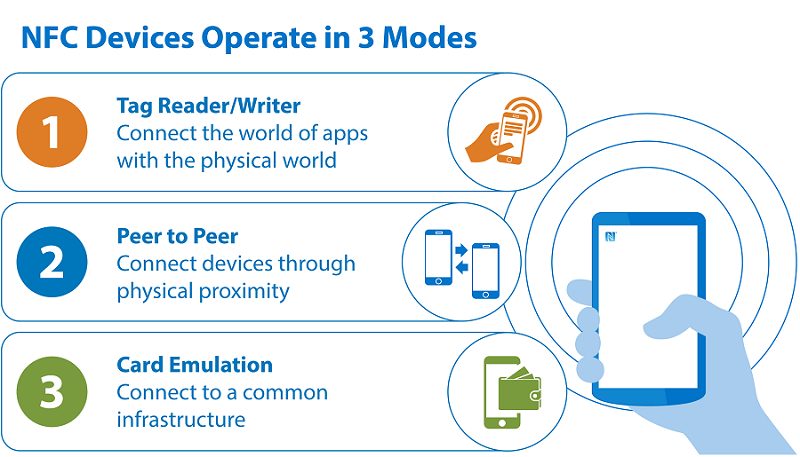
\includegraphics[scale=1.5]{bilder/nfc_modes.png}
\end{center}
\caption{Die drei Betriebsmodi von NFC. Quelle: \citep{NFCWhat}.}
\label{fig:nfc_modes}
\end{figure}

\subsection{Sensoren}
\label{subsec:sensors}

\subsubsection{Beschleunigungssensor}
\label{subsec:accelerometer}
Beschleunigungssensoren (engl. accelerometer) messen die Beschleunigung, der sie zum Zeitpunkt der Messung ausgesetzt sind. In vielen mobilen Geräten sind Beschleunigungssensoren verbaut, die entlang der drei Achsen des Gerätes Beschleunigungsvektoren messen können. Dabei wird das Standardkoordinatensystem aus Abbildung \ref{fig:coordinate_system} verwendet. Ein einfacher Anwendungsfall wäre \zb eine Applikation, die das Schütteln des Gerätes durch eine alternierende Beschleunigung erkennt.

\begin{figure}[ht]
\centering
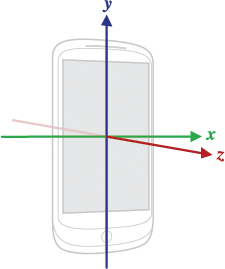
\includegraphics[scale=0.65]{bilder/coordinate_system.png}
\caption{Das Standardkoordinatensystem für Sensoren mobiler Geräte. Quelle: \citep{AndroidSensors}.}
\label{fig:coordinate_system}
\end{figure}

Die Beschleunigungswerte werden mit einer bestimmten \textit{Frequenz} gemessen, die zwischen verschiedenen Sensoren und Implementierungen variieren kann. Ebenso kann sich die \textit{Auflösung} unterscheiden, also die Genauigkeit, mit der die Werte ermittelt werden. Einen Einfluss auf die Messwerte hat die Erdbeschleunigung von \(g=\SI{9.81}{\meter\per\second\square}\), die je nach Orientierung des Gerätes auf eine oder mehrere Achsen wirkt. Ein anschauliches Beispiel dazu findet sich in der Android-Dokumentation. Angenommen wird ein Gerät, das flach auf einem Tisch liegt \citep{AndroidSensors}:
\begin{itemize}
\item Beim Beschleunigen des Gerätes von links (das Gerät bewegt sich nach rechts): positiver Beschleunigungswert auf der X-Achse.
\item Beim Beschleunigen des Gerätes von unten (das Gerät bewegt sich nach oben): positiver Beschleunigungswert auf der Y-Achse.
\item Beim Aufnehmen des Gerätes mit einer Beschleunigung von \(\SI[parse-numbers = false]{x}{\meter\per\square\second}\) wird auf der Z-Achse ein Wert von \(a - g = a - (\SI{-9.81}{\meter\per\square\second}) = a + \SI{9.81}{\meter\per\square\second}\) gemessen, also der Beschleunigung des Gerätes plus die Erdanziehung.
\item Bei ruhiger Lage des Gerätes auf dem Tisch wird eine Beschleunigung von \(\SI{0}{\meter\per\square\second} - (\SI{-9.81}{\meter\per\square\second}) = \SI{9.81}{\meter\per\square\second}\) auf der Z-Achse gemessen.
\end{itemize}

Mit Hilfe eines \textit{linearen Beschleunigungssensors} können die Beschleunigungen entlang der Achsen auch exklusive der Erdanziehung gemessen werden, ohne sie durch Filter nachträglich entfernen zu müssen \citep{AndroidMotionSensors}.

Erweiterte Anwendungen des Beschleunigungssensors finden sich bei Roy und Kollegen, die einen Beschleunigungssensor zum Dekodieren von modulierten Vibrationssignalen verwenden \citep{Nirupam2015}, oder in \citep{Hinckley2004}, wo das Zusammenschlagen ("`Bump"') zweier Tablets mittels Beschleunigungssensoren erkannt wird.

\subsubsection{Gyroskop}
In vielen mobilen Geräten ist neben dem (linearen) Beschleunigungssensor auch noch ein Drehratensensor, meist \textit{Gyroskop} genannt, verbaut. Damit kann die Winkelgeschwindigkeit des Gerätes um die drei Achsen (siehe Abbildung \ref{fig:coordinate_system}) gemessen werden. Während der Beschleunigungssensor die Beschleunigung \textit{entlang} der Achse misst, misst das Gyroskop die Geschwindigkeit \textit{um} die Achse. 

Die Rohwerte beschreiben die Rotationsrate in \si{\radian\per\second}, wobei meist eine Integration der Werte vorgenommen wird, um Winkeländerungen über feste Zeitfenster hinweg zu bestimmen. Zudem gibt es Störfaktoren, die durch die Kombination des Gyroskops mit anderen Sensoren korrigiert werden können \citep{AndroidMotionSensors}. 

Ein anschaulicher Anwendungsfall für das Gyroskop wäre \zb eine Spin-the-bottle-App, in der die Drehung des Smartphones um die Z-Achse eine Flaschendrehung simuliert. Schon Rekimoto machte 1996 Gebrauch von Gyroskopen in tragbaren Geräten, um durch leichte Neigung des Gerätes Menüeinträge durchzuschalten \citep{Rekimoto1996}.

Das Gyroskop misst nur die Änderungsrate um die Achsen des Gerätes ohne weiteren Kontext. Im nächsten Kapitel wird gezeigt, wie auch die Lage des Gerätes im Raum bestimmt werden kann.

\subsubsection{Magnetometer und Orientierung}
Um zu bestimmen, welche Lage ein Gerät relativ zu einem Referenzkoordinatensystem hat, kann ein Orientierungssensor benutzt werden. Dabei handelt es sich um einen Softwaresensor, der die Werte des in Kapitel \ref{subsec:accelerometer} beschriebenen Beschleunigungssensors mit den Werten eines \textit{Magnetometers}, der Änderungen in der Stärke des magnetischen Feldes der Erde misst, kombiniert.

Durch Kombination und Transformation dieser Werte können drei Werte ermittelt werden \citep{AndroidPositionSensors}:
\begin{enumerate}
\item \textit{Azimuth}: Winkel zwischen Y-Achse des Gerätes und dem magnetischen Nordpol. Zeigt die Y-Achse zum magnetischen Nordpol, ist der Wert \ang{0}, für Süden \ang{180}, für Osten und Westen \ang{90} bzw. \ang{270}. 
\item \textit{Pitch}: Rotationswinkel um die X-Achse des Gerätes. Wird die positive Z"~Achse in Richtung der positiven Y-Achse bewegt (siehe Abbildung \ref{fig:rotation_axes}), ist der Wert positiv, sonst negativ.
\item \textit{Roll}: Rotation um die Y-Achse des Gerätes. Funktioniert analog zu Pitch, allerdings bezogen auf die X- und Z-Achse des Gerätes.
\end{enumerate}

\begin{figure}[ht]
\centering
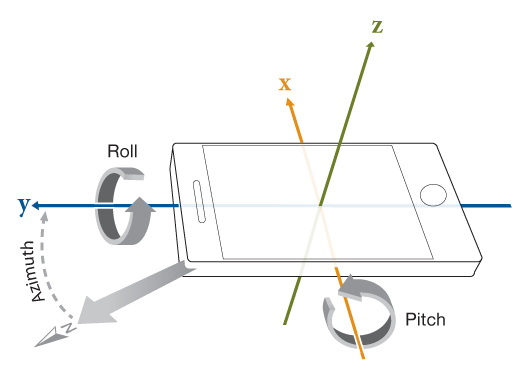
\includegraphics[width=0.7\textwidth]{bilder/device_orientation.jpg}
\caption{Azimuth, Pitch und Roll bei mobilen Geräten. Quelle: \citep{Mathworks2014}.}
\label{fig:rotation_axes}
\end{figure}

Im Gegensatz zu Beschleunigungssensor und Gyroskop beschreiben diese Werte eine Lage im Raum, keine Änderungsrate. Dabei ist der Azimuth-Wert interessant, um \zb Kompass-Apps zu realisieren. Eine Kombination aller drei Werte kann genutzt werden, um die Lage verschiedener Geräte zueinander zu bestimmen.

\subsubsection{Touchscreens}
Ein Nutzer mit Desktop-PC wird seine Eingaben üblicherweise mit Maus und Tastatur machen. Laptops haben die Maus durch ein Touchpad bzw. einen Trackpoint ersetzt, womit der Nutzer Bewegungen des Mauszeigers und teilweise auch Tastendrücke oder einfache Gesten durchführen kann. 

Mit dem iPhone hat Apple als erste Firma ein mobiles Gerät mit Touchscreen entwickelt, das die Bedienbarkeit deutlich interaktiver und simpler gestaltete als Konkurrenzprodukte, deren Design noch immer im Desktop-Stil gehalten wurde. Dadurch wurden auch Gesten wie \zb\textit{pinch} zum Vergrößern von Fotos ermöglicht \citep[42]{Banga2014}. Heute besitzen in der Regel alle Smartphones und Tablets einen Touchscreen, aber auch größere Geräte werden inzwischen mit Touchscreens ausgestattet.

Es gibt verschiedene Technologien, um Touchscreens zu realisieren. Walker unterscheidet zwischen sechs Basistechnologien von Touchscreens \citep[35]{Walker2015}:
\begin{enumerate}
\begin{small}
\item kapazitiv
\item resistiv 
\item akustisch
\item optisch
\item eingebettet
\item andere
\end{small}
\end{enumerate}

Jede dieser Technologien hat verschiedene Vor- und Nachteile. Eines der Schlüsselfeatures für Touchscreens ist die \textit{Multitouch}"=Fähigkeit, also die Möglichkeit, mehrere simultane Berührungen auf einem Touchscreen gleichzeitig zu erkennen \citep[39]{Walker2015}.

Kapazitive Displays, die in den meisten mobilen Geräten verbaut sind, besitzen theoretisch keine Limitierung für die Anzahl der Multitouch-Punkte, sind aber in der Skalierung der Größe begrenzt. Große Displays wie der Microsoft PixelSense sind mit Infrarot-Touchscreens ausgestattet, die zwar 32 und mehr Multitouch-Punkte erkennen und in der Größe gut skalieren, dafür aber anfällig für Störungen bei heller Beleuchtung (\zb unter freiem Himmel) sind.

Resistive Displays erkennen im Gegensatz zu kapazitiven auch die Berührung mit einem Stylus oder anderen spitzen Objekten, dafür fehlt hier die Multitouch"=Unterstützung. Zudem ist mehr Kraftaufwand beim Berühren des Touchscreens erforderlich \citep[47,56,76]{Walker2015}.

Bei der Gestaltung von Multiscreen-Interaktionen, die auf Touchscreens basieren, müssen diese Einschränkungen berücksichtigt werden. Für die Eingabe längerer Texte auf Touchscreens gibt es zwar verschiedene Lösungen, allerdings konnten mobile Geräte Desktop-PCs mit Keyboard und Maus im Sinne benutzerfreundlicher Interaktion für diesen Fall bisher nicht ablösen. \citep[46]{Banga2014}.

\subsubsection{Audio und Video}
Mobile Geräte sind in der Regel mit Mikrofonen und Kameras ausgestattet, für PCs und Smart TVs können diese günstig zugekauft werden. Übliche Nutzungsszenarien für  Mikrofone und Kameras sind die Aufnahme von Bildern, Videos und Tondateien oder (Video)-Telefonie.

In Kapitel \ref{subsec:ausgabe} wird gezeigt, wie Shirazi die Kamera als Sensor einsetzt, um modulierte Lichtsignale zu empfangen und eine entsprechende Systemreaktion auszulösen. Aumi und Kollegen demonstrieren mit ihrem DopLink-System die Möglichkeit, mittels Mikrofon einen Dopplereffekt zu erkennen. Dadurch kann die Bewegung eines mobilen Gerätes erkannt werden, das ein Ultraschallsignal aussendet. Über diesen Mechanismus wird die Verbindung zwischen den Geräten aufgebaut \citep{Aumi2013}.

\subsection{Ausgabe}
\label{subsec:ausgabe}
Im Gegensatz zu den vielfältigen Sensoren zur Messung von Nutzeraktionen in Kapitel \ref{subsec:sensors} ist das Feld möglicher Ausgaben für Systemreaktionen überschaubar. 

Alle Geräteklassen ermöglichen schon per Definition in Kapitel \ref{sec:multiscreen} eine Bildschirmausgabe. Zwar können Größe und Form des Bildschirms stark variieren, visuelles Feedback ist jedoch generell möglich und in der Regel mittels der jeweiligen GUI-Frameworks einfach zu realisieren.

Fast ebenso universell vorhanden ist die Möglichkeit für akustisches Feedback.  Als Kommunikations- bzw. Unterhaltungsgeräte besitzen Geräte der Klassen Smartphone und Tablet in aller Regel eine Audioausgabe. Auch Laptops und kleinere Smart TVs sind mit Audioequipment ausgestattet. Lediglich Desktop PCs oder große Leinwände können unter Umständen kein akustisches Feedback liefern. 

Mobile Geräte sind zudem häufig mit einem Vibrationsmotor ausgestattet, der in Geräten der anderen Klassen meist nicht vorhanden ist. Vibration kann als Systemreaktion eingesetzt werden, um \zb Tastendrücke auf einem Touchscreen mit einer gefühlten Haptik zu versehen. Oliveira und Kollegen haben gezeigt, dass sich damit sogar eine Braille-Tastatur mittels Touchscreens realisieren lässt \citep{Oliveira2011}. Zudem kann Vibration in Kombination mit anderen Ausgaben eingesetzt werden, \zb als Ergänzung zu akustischem Feedback, um in lauten Umgebungen trotzdem die Aufmerksamkeit des Nutzers zu erlangen. Für Geräte, die sich nicht in unmittelbarer Nähe des Nutzers befinden, ist diese Art von Feedback nicht nutzbar.

Tablets und Smartphones sind teilweise mit einer ansteuerbaren Lampe ausgestattet. Neben typischen Anwendungsfällen wie Taschenlampen- oder Foto-Apps haben Shirazi und Kollegen 
gezeigt, wie ein Anwender mittels seiner Smartphone-Lampe einen Pointer auf einem großen Display steuern kann, dessen Kamera das Lichtsignal aufnimmt und verarbeitet \citep{Shirazi2009}. Nichtsdestotrotz sind die Einsatzmöglichkeiten in Multiscreen-Interaktionen eher eingeschränkt.

\chapter{Modell für Multiscreen-Interaktionen}
\label{ch:modell}
\section{Herausforderungen}
\label{sec:herausforderungen}
Die in Kapitel \ref{sec:msp-patterns} vorgestellte Patternvorlage dient als Basis, das Wissen zu den einzelnen Multiscreen-Patterns einheitlich und strukturiert erfassen zu können. Während Aspekte wie Problem, Lösung oder Anwendungskontext mit natürlicher Sprache bzw. mittels Checkboxen und Listen erfasst werden können, ist es deutlich schwieriger, eine konsistente, strukturierte Form für die Erfassung der technischen Realisierung von Patterns, also der Gestaltung des "`Wie"', zu finden.

Für verschiedene Patternsammlungen wurde bei der Dokumentation der technischen Umsetzung dabei sehr unterschiedlich vorgegangen. Gamma und Kollegen verwenden eine Mischung aus OMT\footnote{Die \ac{OMT} ist eine Anfang der Neunzigerjahre entwickelte Objekt-Modellierungssprache.}- und Interaktionsdiagrammen sowie Code-Beispielen in C++ und SmallTalk, um die strukturelle und semantische Umsetzung der Patterns zu dokumentieren \citep{Gamma1995}. Durch den Einsatz gängiger Programmier- und Modellierungssprachen sind die Patterns für Entwickler einfach nachzuvollziehen und umzusetzen.

Die Patternsammlungen von \cite{Tidwell2010}, \cite{Yahoo2015} und \cite{Welie2008}, die sich mit der Lösung wiederkehrender Probleme bei der Gestaltung von Applikations"= und Webinterfaces befassen, nutzen natürlichsprachliche Beschreibungen, meist ergänzt um  Beispiele in Form von Screenshots. Auf Formalismen zur abstrakten Beschreibung von GUI- und Interaktionsdesign wird hier gänzlich verzichtet, da die Patterns keine strikten Regeln und keine Schritt-für-Schritt Anleitungen für das Interface-Design sein sollen \citep[xviii]{Tidwell2010}. 

Bei der Beschreibung der technischen Aspekte von Multiscreen-Patterns ergeben sich  besondere Herausforderungen. Neben der \acs{GUI}-Gestaltung müssen auch Interaktionsmodalitäten, Kommunikationsprotokolle oder technische Voraussetzungen, unter denen der Einsatz bestimmter Patterns überhaupt erst möglich ist, berücksichtigt werden. Zudem steht im Zentrum jedes Multiscreen-Patterns eine oft komplexe Geste, deren Erkennungsalgorithmus beschrieben werden muss. Daraus ergibt sich, dass Multiscreen-Patterns als Kommunikationsmittel zwischen Designern, Entwicklern, Softwarearchitekten und anderen Projektbeteiligten verstanden und genutzt werden müssen. Dabei sollten einige zentrale Fragen durch die technische Beschreibung des Patterns beantwortet werden, wie bspw.:
\begin{itemize}
\item Kann das Pattern in einer gegebenen Infrastruktur eingesetzt werden?
\item Gibt es technische Einschränkungen bei der Umsetzung des Patterns?
\item In welcher Form interagiert der Nutzer mit dem Gerät?
\item Was für Eingaben kann der Nutzer tätigen, welche Systemreaktionen gibt es?
\item Welche Systemkomponenten können an welcher Stelle wiederverwendet / kombiniert werden?
\item Wie sieht das Kommunikationsprotokoll aus, das die beteiligten Geräte implementieren müssen? 
\item Welche Daten werden übermittelt?
\end{itemize}
Um ein einheitliches Modell zu schaffen, das die Beantwortung dieser Fragen für jedes Pattern ermöglicht, wird sich die Analyse in diesem Kapitel mit Publikationen zum Thema Multiscreen-Interaktion auseinandersetzen, die für verschiedene Multiscreen-Szenarien bereits eine theoretische oder praktische technische Realisierung beschreiben. Für diese heterogenen Konzepte wird anschließend eine gemeinsame Abstraktion erarbeitet. Als Leitlinie für die Analyse und Modellierung werden im folgenden Kapitel zunächst konkrete Anforderungen an das Modell formuliert.

\section{Anforderungen an das Modell}
\label{sec:requirements}
Aus dem Projektziel von \sysplace und den zentralen Forschungsfragen in Kapitel \ref{sec:sysplace} sowie den bereits erarbeiteten Patterns in Kapitel \ref{sec:msp-patterns} lassen sich Anforderungen an das Modell aus Sicht verschiedener Nutzergruppen ableiten.
Wie in Kapitel \ref{sec:msp-patterns} beschrieben, zerfällt ein Multiscreen-Pattern in die Durchführung einer Geste und eine darauf folgende Systemreaktion. Die konzeptionelle Erfassung von Gesten entsprechend der ersten Forschungsfrage in Kapitel \ref{sec:sysplace} ist durch das Patterntemplate bereits vorgenommen worden (vgl. Anhang \ref{a:patterntemplate}). 

Soll ein Pattern in einer Multiscreen-Anwendung realisiert werden, wird sich für den Entwickler die Frage stellen, wie die entsprechende Geste technisch erkannt werden kann. Das Patterntemplate in Anhang \ref{a:patterntemplate} beschreibt unter "`Wie"' zwar allgemein die Durchführung der Geste und unter "`Technisches"' mögliche Technologien zur Erkennung von Gesten, trifft allerdings keine Aussage darüber, wie diese Technologien konkret eingesetzt und ggf. kombiniert werden müssen. Zudem werden technische Alternativen für die Erkennung nicht ausreichend berücksichtigt.

Folgende Aspekte sollen durch das Modell daher hinsichtlich der zweiten\footnote{Welche methodisch-/technischen Voraussetzungen sind notwendig, um diese Interaktionen zu unterstützen?} und dritten\footnote{Welche Entwicklungsverfahren, -werkzeuge und -modelle und Voraussetzungen muss die zugrunde liegende Softwarearchitektur des Gesamtsystems mitbringen, um die Szenarien zu unterstützen?} Forschungsfrage beschrieben werden:
\begin{itemize}
\item Die zu verarbeitenden Eingaben des Nutzers in Form von Sensordaten oder anderen Systemevents;
\item Hard- und Softwarevoraussetzungen, unter denen diese Daten verfügbar sind;
\item Abstrakte Beschreibung des Erkennungsalgorithmus einer Geste auf Basis von Sensordaten;
\item Alternative Erkennungsmöglichkeiten und deren Implikationen;
\item Möglichkeiten zur Einschränkung, unter welchen Umständen eine Geste erkannt wird;
\item Kommunikationsprotokolle zwischen Geräten für die Erkennung geräteübergreifender Gesten;
\item Wiederverwendbarkeit von Teilkomponenten.
\end{itemize}
Diese Aspekte sollten unabhängig von konkreten Technologien modelliert werden, sodass eine Umsetzung auf verschiedenen Plattformen möglich ist. Zudem soll eine Repräsentation gewählt werden, deren Syntax und Regeln einem Entwickler intuitiv verständlich sind.

Nachdem eine Geste durch das System erkannt wurde, folgt eine Systemreaktion entsprechend der fünf Kategorien\footnote{\textit{Connect} (Geräte Verbinden), \textit{Give} (Daten übermitteln), \textit{Take} (Daten empfangen), \textit{Exchange} (Daten austauschen), \textit{Extend} (Geräte koppeln).} aus Kapitel \ref{sec:msp-patterns}. Dabei handelt es sich meist nicht um einfache Reaktionen wie \zb Textausgaben auf dem Bildschirm, sondern um komplexere Abläufe, die eventuell weitere Ein- und Ausgaben oder Datenverarbeitung beinhalten. Eine allgemeine Beschreibung der Systemreaktion sowie möglicher Erfolgs- und Fehlerfälle ist im Patterntemplate unter "`Wie"' zu finden, allerdings wird hier nur ein konzeptioneller Überblick gegeben, der Detailgrad reicht für die Beantwortung der Forschungsfragen zwei\footnote{Welche methodisch-/technischen Voraussetzungen sind notwendig, um diese Interaktionen zu unterstützen?} und drei\footnote{Welche Entwicklungsverfahren, -werkzeuge und -modelle und Voraussetzungen muss die zugrunde liegende Softwarearchitektur des Gesamtsystems mitbringen, um die Szenarien zu unterstützen?} nicht aus.

Aus Sicht eines Interaktionsdesigners sollten daher folgende Aspekte modelliert werden:
\begin{itemize}
\item Vollständige Ablaufbeschreibung der Systemreaktion,
\item eventuelle Vor- und Nachbedingungen der Systemreaktion,
\item mögliche Interaktionen des Nutzers,
\item mögliche Rückmeldungen des Systems an den Nutzer und
\item Implikationen der gewählten Geste auf die Abläufe der Multiscreen"=Anwendung.
\end{itemize}
Jede Kategorie hat eigene Implikationen, die von dem Modell erfasst werden sollten, wie \zb uni- und bidirektionale Datenübertragung oder der Verbindungsaufbau zwischen Geräten. Interaktionsdesigner gestalten diese Abläufe zwar konzeptionell, die technische Realisierung aber übernehmen Entwickler. Aus Entwicklersicht kommen noch technische Aspekte hinzu, die im Modell berücksichtigt werden müssen:
\begin{itemize}
\item Benötigte Objekte und deren Datenfluss im System,
\item Implikationen verarbeiteter Daten auf den weiteren Programmfluss,
\item Zustand vor und nach der Systemreaktion und
\item Beschreibung möglicher Alternativen oder Fehlerfälle.
\end{itemize}
Da das Modell an dieser Stelle ein wichtiges Kommunikationsmittel zwischen Entwicklern und Interaktionsdesignern darstellt, soll eine für beide verständliche Repräsentation eingesetzt werden.

Zusätzlich zu den Anforderungen, die sich aus dem Patterntemplate ergeben, sind  noch weitere, generelle Aspekte für die Modellierung relevant. Die Erfassung und Überarbeitung von Patterns ist ein kontinuierlicher Prozess. Es ist möglich, dass weitere Patterns in die Sammlung aufgenommen oder alternative Lösungsansätze erfasst werden. Das Modell sollte daher nicht nur den aktuellen Umfang der Sammlung abbilden können, sondern offen für Erweiterungen innerhalb des Kontexts der Multiscreen-Interaktion sein.

Per Definition bieten Patterns keine fertige Lösung für ein konkretes Problem, sondern abstrakte Lösungsansätze für wiederkehrende Problemtypen (vgl. Kapitel \ref{sec:msp-patterns}). In der Praxis bedeutet das, dass Anwender von Patterns eine Instanz des Modells erstellen müssen, die eine Realisierung der vorhandenen Anwendungsfälle ermöglicht. Das Projektziel in Kapitel \ref{sec:sysplace} definiert als Anwender der Patterns kleine und mittelständische Unternehmen. Damit diese mit dem Modell arbeiten können, sollten die eingesetzten Modellierungssprachen und -werkzeuge frei verfügbar sein und kein umfangreiches Vorwissen benötigen.

Je nachdem in welchem Multiscreen-Szenario Patterns eingesetzt werden, sind eventuell Geräte bestimmter Klassen vorhanden. Das Modell sollte diesen Punkt berücksichtigen und die Beziehung zwischen einem konkret modellierten Lösungsansatz und den dafür benötigten Mindestanforderungen an Hard- und Software abbilden.

\section{Erarbeitung des Modells}
Die folgenden Unterkapitel beschreiben schrittweise das erarbeitete Modell. Dabei wird jeweils nach demselben Schema vorgegangen:
\begin{enumerate}
\item Kurzer Überblick über den Fokus des Teilmodells und die Einordnung in das Gesamtmodell,
\item Präsentation und Erklärung des erarbeiteten Teilmodells und
\item ausführliche Begründung für die Modellierungsentscheidungen.
\end{enumerate}
Zur Modellierung werden Diagramme der \ac{UML} in der aktuellen Version 2.5 verwendet. Die \acs{UML} dient zur Modellierung, Dokumentation, Spezifizierung und Visualisierung komplexer Systeme, unabhängig von deren Fachdomäne. Sie liefert Notationselemente für die statischen und dynamischen Modelle von Analyse, Design und Architektur und unterstützt insbesondere ob\-jekt\-ori\-en\-tier\-te Vorgehensweisen 
\citep[4]{UML2012}.

Laut Rupp und Kollegen ist die \acs{UML} zudem \citep[4]{UML2012}
\begin{itemize}
\item nicht vollständig,
\item keine Programmiersprache,
\item keine rein formale Sprache,
\item kein vollständiger Ersatz für Textbeschreibung und
\item weder Methode noch Vorgehensmodell.
\end{itemize}
All diese Eigenschaften passen zu den Herausforderungen und Anforderungen an das Modell (vgl. Kapitel \ref{sec:herausforderungen} und \ref{sec:requirements}). UML ermöglicht es, die technische Komplexität von Multiscreen-Patterns zu visualisieren und dadurch die Textbeschreibungen um detaillierte Diagramme zu ergänzen. Zudem sind mit StarUML, UMLet, Eclipse etc. viele frei verfügbare Werkzeuge für die UML"=Modellierung vorhanden. Die weite Verbreitung von \ac{UML} trägt dazu bei, dass die gängigen Diagrammtypen von den meisten Entwicklern gelesen werden können. 

Verschiedene Aspekte des Modells werden mit dem jeweils geeigneten Diagrammtyp dargestellt. Der UML-Standard legt nicht exakt fest, welche Elemente in welchem Diagrammtypen vorkommen dürfen \citep[15]{UML2012}. Bevor in dieser Arbeit ein Diagrammtyp erstmals verwendet wird, wird kurz beschrieben, in welcher Form er verwendet wird und wo eventuelle Abweichungen zur gängigen Verwendung von UML vorgenommen wurden.

Das Ergebnis ist ein \textit{semi-formales} Modell, das \textit{visuell} repräsentiert wird und \textit{statische} sowie \textit{dynamische Aspekte} der Multiscreen-Interaktion abbildet.

\subsection{Rahmenmodell}
\label{subsec:model_overview}
Die SysPlace-Patterns beschreiben zwar jeweils nur eine Geste mit einer darauf folgenden komplexen Systemreaktion (siehe Kapitel \ref{sec:msp-patterns}), müssen aber bei der Realisierung stets in einen Applikationskontext eingebettet werden. Bei näherer Betrachtung der fünf Kategorien fällt zudem auf, dass hier zwar keine \textit{Pattern Language}\footnote{Borchers beschreibt eine Pattern Language als einen gerichteten Graphen, in dem Patterns höherer Ebenen auf Patterns niedrigerer Ebenen verweisen, wodurch sich eine Hierarchie von gemeinsam nutzbaren Patterns ergibt \citep{Borchers2000}.} vorliegt, da alle Patterns das gleiche Abstraktionsniveau haben und es keine hierarchische Struktur zwischen den Patterns gibt, die Patterns der Kategorie "`Connect"' allerdings nur zur Verbindung von Geräten genutzt werden, während die Patterns der anderen vier Kategorien in irgendeiner Weise Daten übertragen und somit eine bereits bestehende Verbindung voraussetzen. Dadurch entsteht eine gewisse Abhängigkeit zwischen den Pattern dieser Kategorien. 

Das Rahmenmodell aus Abbildung \ref{fig:model_overview} beschreibt einen Applikationslebenszyklus aus Sicht von Multiscreen-Interaktionen, der die Einsatzgebiete der Patterns berücksichtigt und in Beziehung zueinander setzt. Am Anfang steht immer eine Aktivität zur Verbindung von Geräten (\textit{Connect}), auf die entweder eine sofortige Trennung (\textit{disconnect}) oder eine beliebig oft wiederholte Abfolge von Auswahl- und Transfer-Aktivitäten (\textit{Select} bzw. \textit{Transfer}) folgt, bis irgendwann die Verbindung getrennt und der Anwendungslebenszyklus beendet wird.
\begin{figure}[h]
\centering
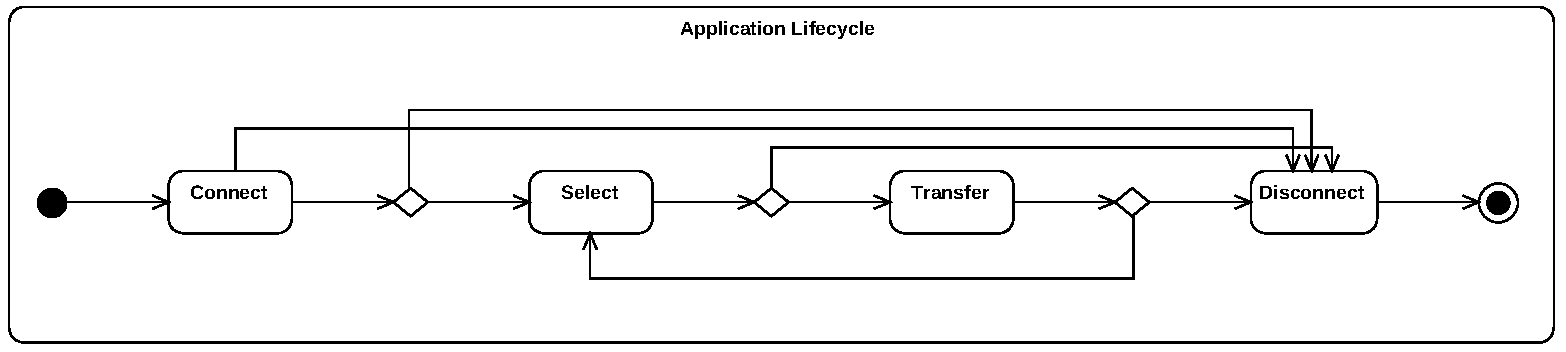
\includegraphics[page=1,width=1\textwidth]{bilder/lifecycle.pdf}
\caption{Rahmenmodell für Multiscreen-Interaktion.}
\label{fig:model_overview}
\end{figure}
Verschiedene Systeme und Konzepte, die Multiscreen-Szenarien realisieren, implementieren diesen Ablauf komplett oder in Teilen und bilden die Grundlage für die Erstellung des Modells. Die wichtigsten Konzepte werden im Folgenden näher betrachtet.

Holmquist und Kollegen stellen das System \textit{Smart-Its Friends} vor, mit dem Geräte um eine externe Komponente erweitert werden können (siehe Abbildung \ref{fig:smart_its_friends}), die einen impliziten (durch Annäherung) oder expliziten (durch eine Schüttel-Geste) Verbindungsaufbau zwischen diesen Geräten ermöglicht \citep{Holmquist2001}. Nachdem eine direkte Verbindung zwischen den Geräten aufgebaut wurde, bleibt es der Anwendung überlassen, diesen Kommunikationskanal zur Übertragung anwendungsspezifischer Nutzdaten zu verwenden. Der Verbindungsabbau findet entweder statt, wenn verbundene Geräte sich nicht mehr in Sendereichweite befinden oder wenn die Applikation die Verbindung aktiv schließt.
\begin{figure}[h]
\centering
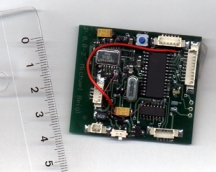
\includegraphics[scale=1]{bilder/smart_its_friends.png}
\caption{Smart-Its Friends Sender / Empfänger. Quelle: \citep{Holmquist2001}.}
\label{fig:smart_its_friends}
\end{figure}

Aus Sicht von Smart-Its Friends erfolgt also immer zuerst der Verbindungsschritt, also die Aktivität \textit{Connect}. Danach kann entweder ein \textit{Disconnect} stattfinden (wenn die Geräte auseinander bewegt werden) oder es ist möglich, dass die Anwendung solange Daten auswählt und transferiert, bis ein Zustand erreicht wird, in dem der \textit{Disconnect} durch die Anwendung erfolgt. Diese möglichen Abläufe finden sich im Modell in Abbildung \ref{fig:model_overview} wieder.

Dachselt und Buchholz entwerfen ein Multiscreen-Szenario, das einen ähnlichen Ablauf realisiert, obwohl andere Technologien und Gesten eingesetzt werden \citep{Dachselt2009}. Die Interaktion findet hier zwischen einem Smartphone und einem Smart TV statt (siehe Abbildung \ref{fig:throw_and_tilt}). Betritt ein Anwender den Raum, wird automatisch eine Wi-Fi- oder Bluetooth-Verbindung zwischen den beiden Geräten hergestellt. Eine Wurfgeste des Smartphones in Richtung des Smart TVs überträgt die Bilder des Smartphones auf das TV-Gerät. Anschließend können die einzelnen Bilder auf dem Smart TV durch Kippen (\textit{Tilt-Geste}\footnote{Eine ausführliche Beschreibung der Tilt-Geste zum Steuern von Menüs findet sich in \citep{Rekimoto1996}.}) des Smartphones durchgeschaltet werden. Eine ruckartige Geste zum Körper (\textit{Fetch-Back-Geste}) ermöglicht den Transfer von Bildern in die andere Richtung (vom Smart TV auf das Smartphone), das Verlassen des Raumes schließt die Verbindung.
\begin{figure}[h]
\centering
\subfigure[Auswahl eines Bildes]{
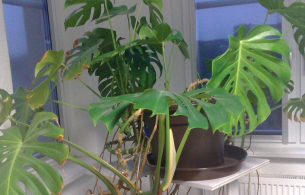
\includegraphics[width=.31\textwidth]{bilder/throw_tilt_1.png}
}
\subfigure[Wurf-Geste zur Übertragung]{
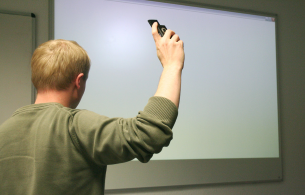
\includegraphics[width=.31\textwidth]{bilder/throw_tilt_2.png}
}
\subfigure[Anzeige auf dem Smart TV]{
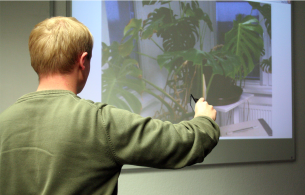
\includegraphics[width=.31\textwidth]{bilder/throw_tilt_3.png}
}
\caption{Wurf-Geste zur Interaktion zwischen Smartphone und Smart TV. Quelle: \citep{Dachselt2009}.}
\label{fig:throw_and_tilt}
\end{figure}

Auch dieser Ablauf lässt sich durch das Modell beschreiben:
\begin{itemize}
\item Aufbauen einer Verbindung durch Betreten des Raumes (\textit{Connect}),
\item Auswahl zu übertragender Dateien (\textit{Select}),
\item Wurf-Geste zum Anstoßen der Übertragung (\textit{Transfer}),
\item Wiederholte Tilt-Gesten zum Durchschalten der Fotos (\textit{Select / Transfer}),
\item Fetch-Back-Geste zum Empfangen von Daten des TV-Gerätes (\textit{Select / Transfer}) und
\item Abbauen der Verbindung durch Verlassen des Raumes (\textit{Disconnect}).
\end{itemize}

In diesem Ablauf gibt es eine Wiederholung der Schritte \textit{Select} und \textit{Transfer}, was im Modell in Abbildung \ref{fig:model_overview} berücksichtigt wird. Nach jedem Transfer wartet das Gerät auf weitere Eingaben, erst das Verlassen des Raumes beendet den Ablauf. Zudem gibt es hier noch eine weitere Ergänzung. Die Tilt-Geste überträgt statt Daten des Nutzers nur einen Steuerbefehl, der das Smart TV zum Weiterschalten der Fotos veranlasst. Die Selektion erfolgt hier implizit, weil durch die Geste nur der Zustand auf dem Smart TV verändert wird, aber keine neuen Fotos übertragen werden. Auf diese Details wird in den Kapiteln \ref{sec:select} und \ref{subsec:transfer} näher eingegangen.

\begin{figure}[h!]
\centering
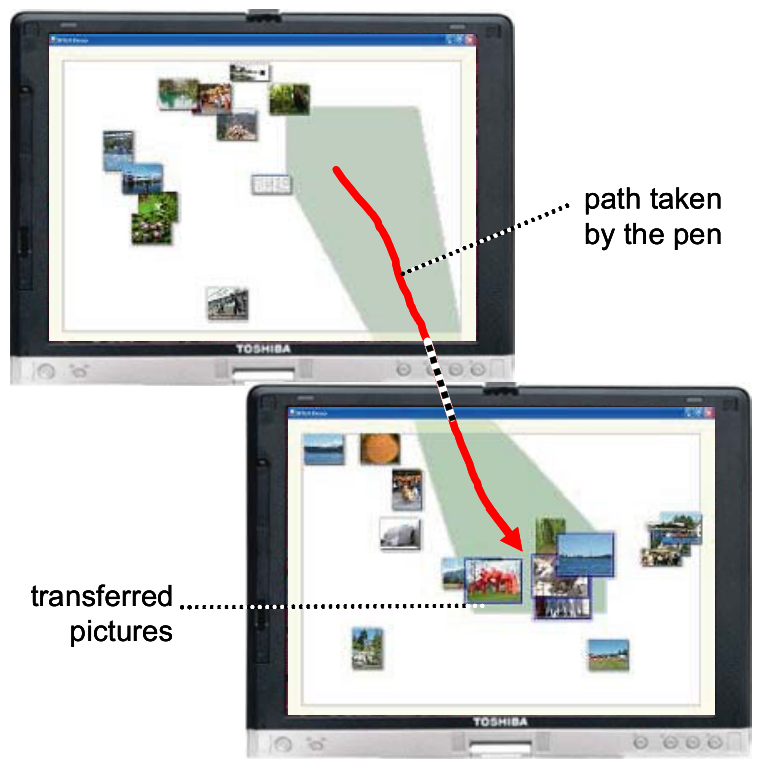
\includegraphics[width=0.5\textwidth]{bilder/stitch_general.png}
\caption{Stitch-Geste zur Übertragung von Bildern. Quelle: \citep{Hinckley2004}.}
\label{fig:stitch_general}
\end{figure}

Eine weitere wichtige Ergänzung findet sich im System \textit{StitchMaster}, das Hinckley und Kollegen entworfen haben \citep{Hinckley2004}. Auch hier wird eine Interaktion zwischen zwei Geräten, diesmal mittels einer sog. \textit{Stitch}-Geste, realisiert. Es werden zwei Geräte nebeneinander positioniert und mit einer Stift-Bewegung von einem auf den anderen Bildschirm verbunden (siehe Abbildung \ref{fig:stitch_general}). Die Selektion von Daten findet vor der Verbindung und Übertragung statt. Durch die anschließende Stitch-Geste wird sowohl die Verbindung zwischen den Geräten aufgebaut als auch die Übertragung von Daten eingeleitet. Die auszuführende Aktion auf dem Zielgerät wird entweder aus der Art der ausgewählten Daten abgeleitet oder durch den Nutzer auf dem Zielgerät explizit ausgewählt. Der Nutzer hat außerdem die Möglichkeit, eine bestehende Verbindung über die Auswahl eines Menüpunkts zu trennen.

Für das Modell kann aus dem System StitchMaster abgeleitet werden, dass bei Verwendung derselben Geste für \textit{Connect} und \textit{Transfer} auch ein alternativer Ablauf eingesetzt werden kann, der in Abbildung \ref{fig:model_overview_alternative} zu finden ist. Die Aktivitäten \textit{Connect} und \textit{Transfer} sind direkt verbunden und finden gemeinsam statt, die Aktivität \textit{Select} ist beiden vorangestellt. Ein wiederholtes Ausführen der Geste würde die Kombination aus Verbindung und Übertragung erneut anstoßen. Ein ähnlicher Ablauf findet sich auch in \citep{Hinckley2003} für Bump-Gesten. Die Bedingung, dass dieselbe Geste zum  Verbinden und Übertragen zum Einsatz kommt, ist auch hier erfüllt.

\begin{figure}[h!]
\centering
\includegraphics[page=2,width=1\textwidth]{bilder/lifecycle.pdf}
\caption{Rahmenmodell mit zusammengefassten \textit{Connect}"= und \textit{Transfer}"=Aktivitäten.}
\label{fig:model_overview_alternative}
\end{figure}

Jede der vier Aktivitäten des Rahmenmodells kann durch Gesten unterstützt werden, wobei die SysPlace-Patterns vor allem die Gestaltung der Aktivitäten \textit{Connect}, \textit{Transfer} und \textit{Disconnect} adressieren. Im folgenden Kapitel wird zunächst die erarbeitete Modellierung der Gestenerkennung beschrieben, bevor die einzelnen Aktivitäten und deren Modellierung im Detail besprochen werden, da diese auf der Gestenerkennung aufbauen.

\subsection{Erkennung einfacher Gesten}
\label{subsec:simple_gesture}
Wie in Kapitel \ref{sec:msp-patterns} beschrieben, besteht ein Multiscreen"=Pattern  aus einer Geste des Nutzers sowie der ausgelösten Systemreaktion. Das SysPlace"=Patterntemplate (siehe Anhang \ref{a:patterntemplate}) sieht zwar eine textuelle und grafische Beschreibung von Gesten vor, gibt allerdings wenig Hinweise über Implementierungsdetails. Um eine Gestenerkennung implementieren zu können, müssen dem Entwickler verschiedene Aspekte bekannt sein:
\begin{itemize}
\item Benötigte Eingabe- und Sensordaten
\item Interpretation / Verarbeitung der Daten
\item Mögliche Einschränkungen für die Erkennung
\item Kommunikationsprotokoll für geräteübergreifende Gesten
\end{itemize}
Soll \zb eine Swipe-Geste erkannt werden, muss ein Touchscreen vorhanden sein, dessen Berührungspunkte ausgelesen werden können. Außerdem ist es eventuell notwendig, Informationen über den Swipe auszuwerten, wie \zb Länge oder Richtung der Bewegung, um diese Werte mit vorgegebenen Einschränkungen wie Mindestlänge oder Bewegungsrichtung zu vergleichen. Dadurch kann entschieden werden, ob die Geste in einem bestimmten Kontext korrekt ausgeführt wurde oder nicht.

Zunächst wird die Modellierung \textit{einfacher Gesten}\footnote{Einfache Gesten werden im Rahmen dieser Arbeit diejenigen Gesten genannt, die auf einem einzelnen Gerät erkannt werden, ohne dass eine Kommunikation mit anderen Geräten stattfindet.} vorgestellt. Im nächsten Kapitel werden darauf aufbauend sog. synchrone Gesten eingeführt und das Modell dahin gehend erweitert, dass auch diese Gesten beschrieben werden können.
\begin{figure}[h]
\centering
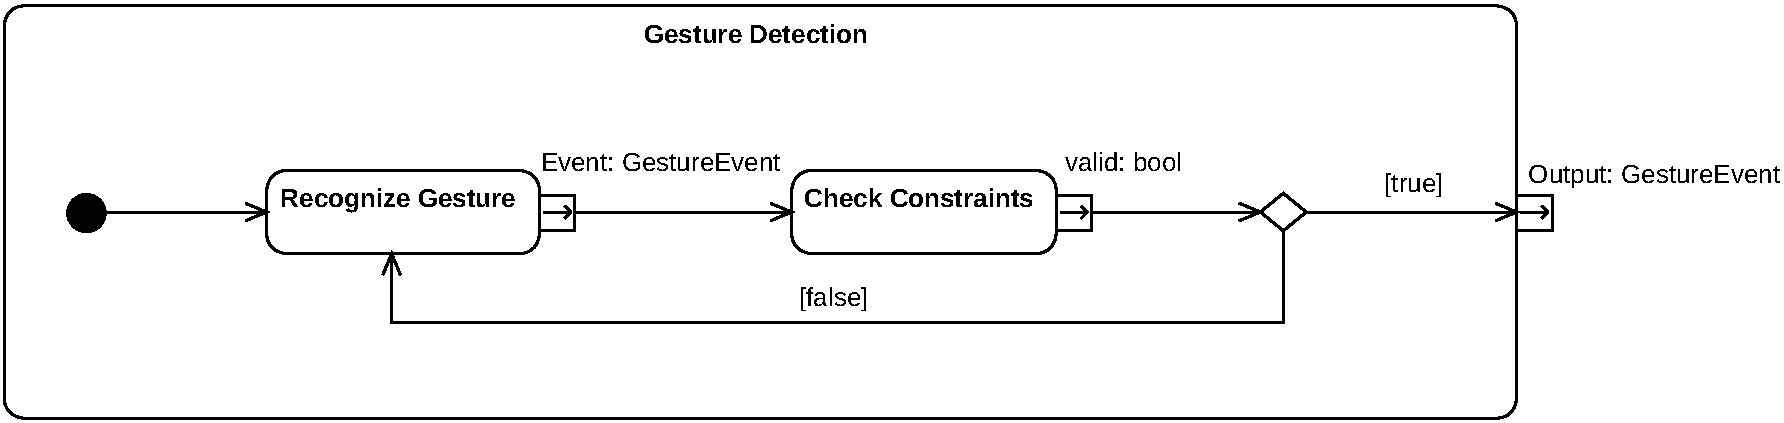
\includegraphics[width=1\textwidth]{bilder/gesture_detection.pdf}
\caption{Modell zur Erkennung einfacher Gesten.}
\label{fig:gesture_detection}
\end{figure}

Das Modell in Abbildung \ref{fig:gesture_detection} ermöglicht es, den Prozess der Erkennung und Einschränkung einfacher Gesten zu beschreiben. Im ersten Schritt (\textit{Recognize Gesture}) erfolgt die Verarbeitung von Sensor- und Eingabedaten, um das grundlegende Muster der Geste zu erkennen. Im zweiten Schritt (\textit{Check Constraints}) wird geprüft, ob die Geste vorgegebenen Einschränkungen (\textit{Constraints}) entspricht. Dementsprechend ist das Ergebnis des ersten Schrittes ein Event, das die Parameter der erkannten Geste beinhaltet (\textit{GestureEvent}), welche im zweiten Schritt mit Einschränkungen an das Grundmuster, also den Anforderungen an ein erfolgreiches Erkennen der Geste, verglichen werden. Die abschließende Übergabe des \textit{GestureEvents} an die weitere Applikationslogik ermöglicht die Steuerung der ausgelösten Systemreaktion oder die Erkennung synchroner Gesten (siehe Kapitel \ref{subsec:synchronous_gesture}).

Die in \citep{Hinckley2004} beschriebene Stitch-Geste zerfällt zunächst in zwei Swipe-Gesten, die auf zwei Geräten unabhängig voneinander erkannt werden müssen und mit dem Modell aus Abbildung \ref{fig:gesture_detection} erfasst werden können. Wie in Abbildung \ref{fig:stitch_general} zu sehen, muss dazu auf einem Gerät ein Swipe in Richtung des Bildschirmrandes erkannt werden und auf dem anderen Gerät ein Swipe vom Rand des Gerätes ausgehend zur Mitte des Bildschirms. Hinckley definiert zudem, dass ein Swipe auf dem ersten Gerät länger als \SI{250}{\milli\second}, auf dem zweiten Gerät länger als \SI{100}{\milli\second} dauern muss und dass eine nicht näher spezifizierte Mindestgeschwindigkeit vorausgesetzt wird, damit die Swipe-Gesten erkannt werden.

In Abbildung \ref{fig:swipe_recognition} ist die Modellierung des ersten Schritts (\textit{Recognize Gesture}) für den Swipe auf einem Gerät exemplarisch vorgenommen worden. Da bei der Erkennung von Gesten auf Sensor- oder andere Eingabe-Events reagiert wird, wird zur Modellierung dieses Schritts ein Zustandsdiagramm verwendet. Benötigte Parameter werden mit \textit{{[}params{]}} gekennzeichnet, benötigte Sensoren oder andere Datenquellen mit \textit{{[}required{]}}. Der Austrittspunkt ist mit der anschließenden Aktivität (hier \textit{Check Constraints: Swipe}) verknüpft, zurückgegebene Daten werden mit \textit{{[}return{]}} gekennzeichnet.
\begin{figure}[h]
\centering
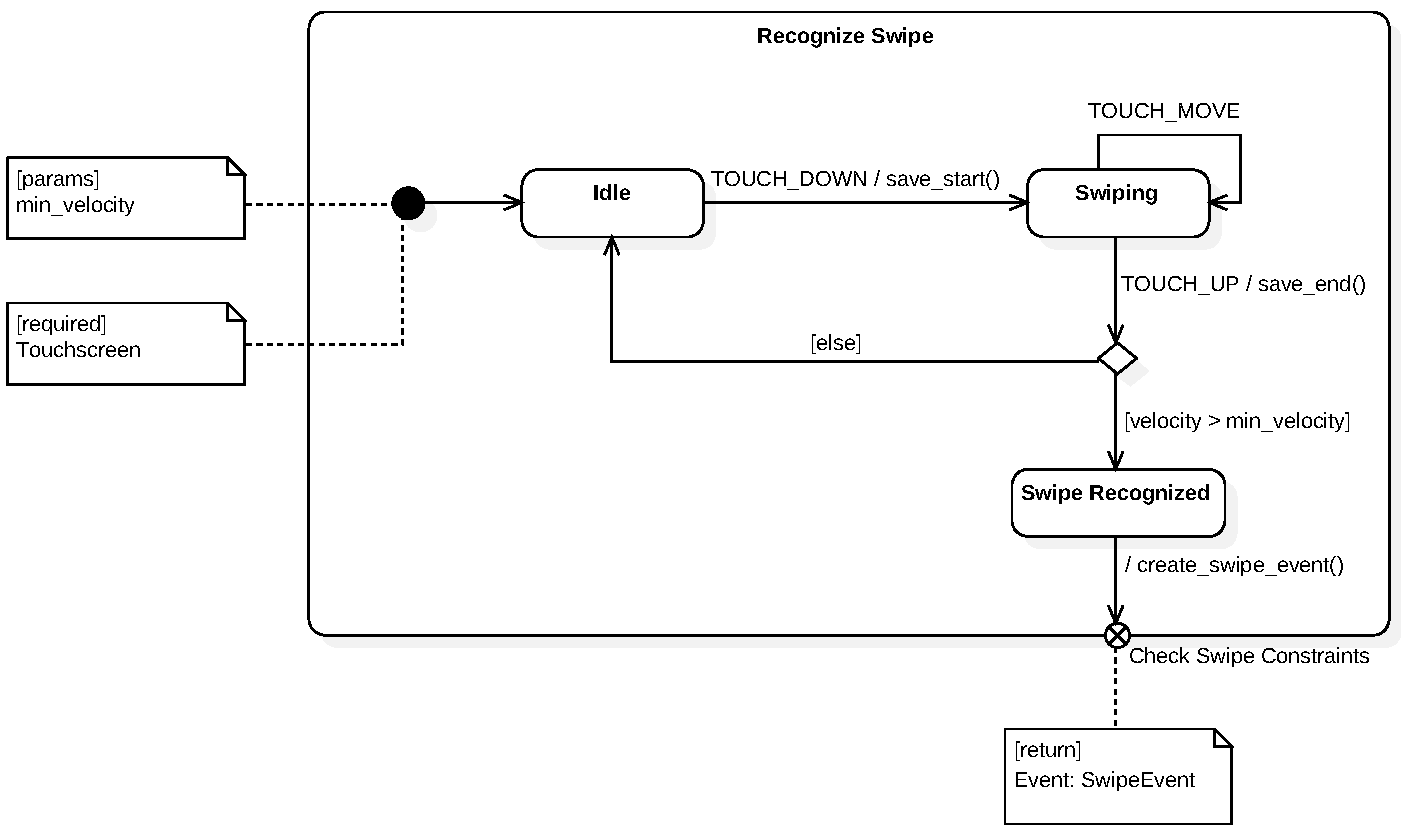
\includegraphics[width=1\textwidth]{bilder/recognize_swipe.pdf}
\caption{Algorithmus zur Erkennung einer Swipe-Geste anhand von Touch-Events.}
\label{fig:swipe_recognition}
\end{figure}

Angelehnt an \citep{Hinckley2004} wird mit \textit{min\_velocity} ein Schwellwert für die Geschwindigkeit als Parameter definiert, außerdem wird ein Touchscreen vorausgesetzt, der mindestens die folgenden Events unterscheiden kann:
\begin{itemize}
\item \textit{TOUCH\_DOWN}: erste Berührung des Bildschirms.
\item \textit{TOUCH\_MOVE}: anhaltende Berührung des Bildschirms.
\item \textit{TOUCH\_UP}: letzte Berührung des Bildschirms.
\end{itemize}

Wurde ein \textit{TOUCH\_DOWN} erkannt, werden Zeitpunkt und Koordinaten des Berührungspunktes gespeichert und auf ein \textit{TOUCH\_UP} gewartet, eventuelle \textit{TOUCH"=\_MOVE}-Events werden ignoriert. Aus den Start- und Endberührungen kann eine Geschwindigkeit errechnet werden, die mit dem Schwellwert \textit{min\_velocity} verglichen wird. Liegt die Geschwindigkeit über dem Schwellwert, wird ein \textit{SwipeEvent} generiert und an den zweiten Schritt, \textit{Check Constraints} (siehe Abbildung \ref{fig:gesture_detection}), übergeben. Ansonsten beginnt die Erkennung von vorne.

Die Modellierung des zweiten Schritts (\textit{Check Constraints}) wurde in Abbildung \ref{fig:check_swipe_constraints} exemplarisch vorgenommen. Hierzu wird ein Aktivitätsdiagramm verwendet, da nicht auf Events reagiert wird, sondern nur prozedural geprüft wird, ob die Parameter des eingehenden Events (hier \textit{SwipeEvent}) vordefinierten Einschränkungen (\textit{Constraints}) entsprechen. In diesem Fall werden analog zu \citep{Hinckley2004} Richtung und zeitliche Dauer des Swipes überprüft. Diese Werte können anhand der Koordinaten und Zeitstempel der ersten und letzten Berührung des Swipes errechnet und mit den erwarteten Werten verglichen werden. Die Definition der Berechnungen findet sich als ergänzende Anmerkung im Diagramm.
In diesem Beispiel wird der Swipe nur dann erkannt, wenn er mindestens \SI{250}{\milli\second} gedauert hat und in Richtung des rechten Bildschirmrandes durchgeführt wurde.
\begin{figure}[h]
\centering
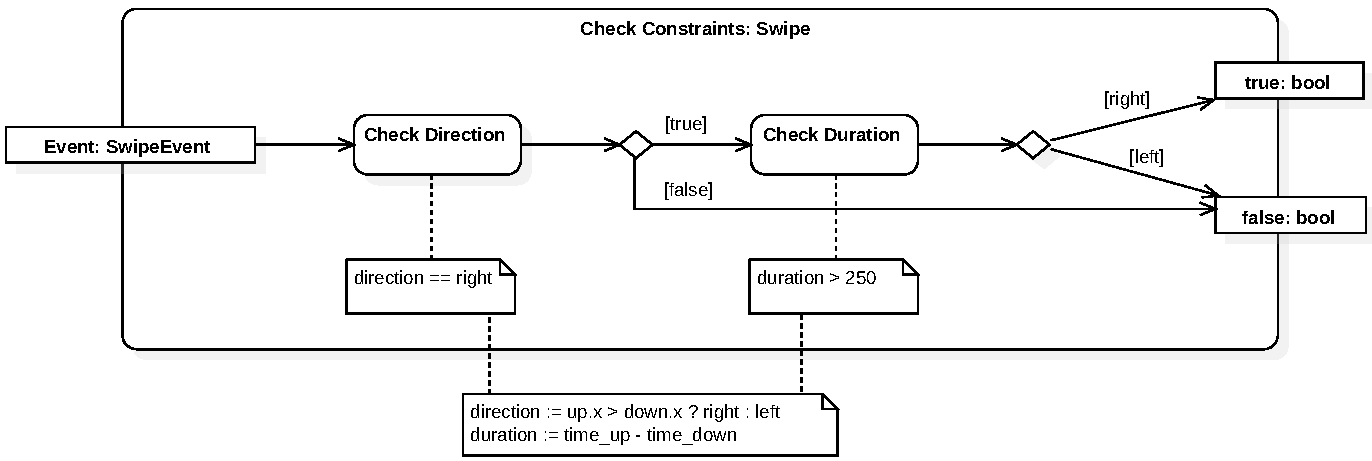
\includegraphics[width=1\textwidth]{bilder/check_swipe_constraints.pdf}
\caption{Vergleich der erkannten Swipe-Geste mit vordefinierten Einschränkungen (\textit{Constraints}).}
\label{fig:check_swipe_constraints}
\end{figure}

Ist die Aktivität \textit{Check Constraints} erfolgreich, also der Rückgabewert \textit{true}, so reicht die \textit{Gesture Detection} aus \ref{fig:gesture_detection} das \textit{SwipeEvent} an die Applikation weiter, die Geste wurde erfolgreich erkannt. Ist die Prüfung nicht erfolgreich, wird die Erkennung erneut gestartet. 

Durch Abwandeln oder Hinzufügen von Parametern für die \textit{Gesture Recognition} und der Definition von \textit{Constraint Checks} lassen sich so eine Vielzahl von Swipe-Gesten einfach beschreiben, wie \zb Teile der Pinch-Geste, die in \citep{Lucero2011}, \citep{Chen2014} oder \citep{Nielsen2014} verwendet wird (siehe Abbildung \ref{fig:pinch}).
\begin{figure}
\centering
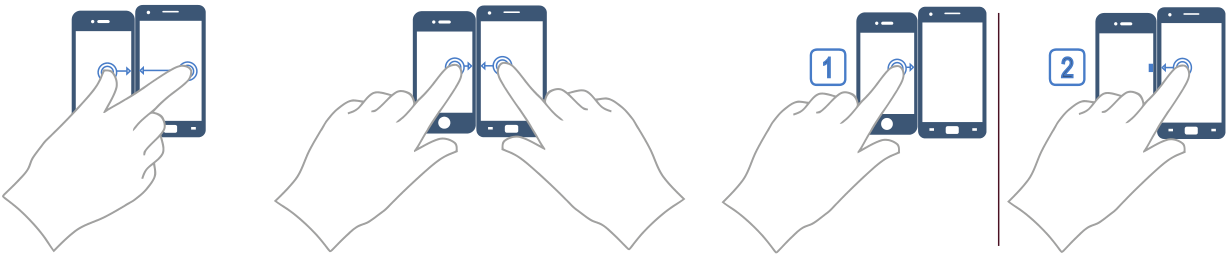
\includegraphics[width=1\textwidth]{bilder/pinch.png}
\caption{Drei Ausprägungen der Pinch-Geste. Quelle: \citep{Nielsen2014}.}
\label{fig:pinch}
\end{figure}

Auch die Erkennung von Gesten, die auf anderen Sensoren basieren, können mit dem Modell beschrieben werden. In \citep{Lucero2011} werden Fotos in einem virtuellen Fotostapel durch eine Tilt-Geste durchgeschaltet, indem das Kippen des Gerätes, das vorher ruhig auf einem Tisch lag, erkannt wird. Dazu wird ein Beschleunigungssensor eingesetzt, der bei ruhiger Lage auf dem Tisch nur die Erdbeschleunigung auf der Z-Achse misst (siehe Kapitel \ref{subsec:accelerometer}). Wird das Gerät nun kippend angehoben, verlagert sich die Beschleunigung auch auf die anderen beiden Achsen, wodurch die Kippbewegung des Gerätes festgestellt werden kann.

Im ersten Schritt (\textit{Recognize Gesture}) wird zunächst das eigentliche Kippen, also der Übergang vom liegenden in den gekippten Zustand, festgestellt. Dazu wird ein Beschleunigungssensor benötigt, der als \textit{required} angegeben wird. Zudem müssen eventuelle Schwankungen (\zb durch leichte Erschütterungen oder leichte Schieflage des Tisches) durch Schwellwerte berücksichtigt werden \citep{Dachselt2009}, die in den \textit{params} definiert werden.

Anschließend kann das resultierende \textit{GestureEvent} (in diesem Fall ein \textit{TiltEvent}, das \zb die Neigungswinkel beinhaltet) noch gegen \textit{Constraints} geprüft werden, da in \citep{Lucero2011} \zb nur horizontales Kippen zum Weiterschalten der Fotos verwendet wird. Das \textit{TiltEvent} wird anschießend an die Applikationslogik übergeben, da es die folgende Systemreaktion eventuell beeinflusst. So schlagen Cho und Kollegen \zb vor, anhand des Neigungswinkels zu entscheiden, wie viele Fotos auf einmal weiter geschaltet werden sollen \citep{Cho2007}. Das Ergebnis ließe sich auch einfach auf \citep{Rekimoto1996} oder \citep{Dachselt2009} übertragen, da beide ebenfalls mit Tilt-Gesten arbeiten.

\subsection{Erkennung synchroner Gesten}
\label{subsec:synchronous_gesture}
Im vorigen Kapitel wurde die Modellierung einfacher Gesten beschrieben, deren Erkennung auf einem einzelnen Gerät stattfindet. Viele Multiscreen-Szenarien beinhalten allerdings Gesten, deren Durchführung mehrere Geräte und Nutzer gleichzeitig einbezieht. Hinckley hat dafür den Begriff der \textit{synchronen Gesten} (engl. \textit{synchronous gestures}) eingeführt, den er wie folgt definiert \citep{Hinckley2003}:
\begin{quote}
These are patterns of activity, contributed by multiple users (or one
user with multiple devices), which take on a new meaning when they occur together in time, or in a specific sequence in time. [\dots\unkern] These patterns could literally occur in parallel and in exact synchrony, or they just might be partially overlapped or even occur in a particular sequence. The key is that complementary portions of a signal are contributed by different devices or participants, and that the signal can only be rec\-og\-nized when these portions are brought together.
\end{quote}

Viele Gesten, wie \zb Bump \citep{Hinckley2003}, Stitch \citep{Hinckley2004}, Pinch (u.a. verwendet in \citep{Lucero2011}, \citep{Chen2014} und \citep{Nielsen2014}) oder das in \citep{Rekimoto2004} vorgestellte System SyncTap fallen unter diese Definition der synchronen Gesten. 

All diese Gesten haben die Gemeinsamkeit, dass zwar auch eine einfache Erkennung pro teilnehmendem Gerät stattfindet, die Erkennung der gesamten synchronen Geste aber zudem einen Abgleich der einzelnen \textit{GestureEvents} und damit auch eine Kommunikation zwischen den einzelnen Geräten erfordert. Abbildung \ref{fig:sync_gesture_detection} zeigt eine Erweiterung des Modells, um synchrone Gesten beschreiben zu können. Zur Darstellung wird ein Sequenzdiagramm verwendet, das üblicherweise zur Visualisierung von Protokollen und Kommunikationsabläufen verwendet wird und hier den zeitlichen Ablauf ausgetauschter Nachrichten anschaulich abbildet.
\begin{sidewaysfigure}
\centering
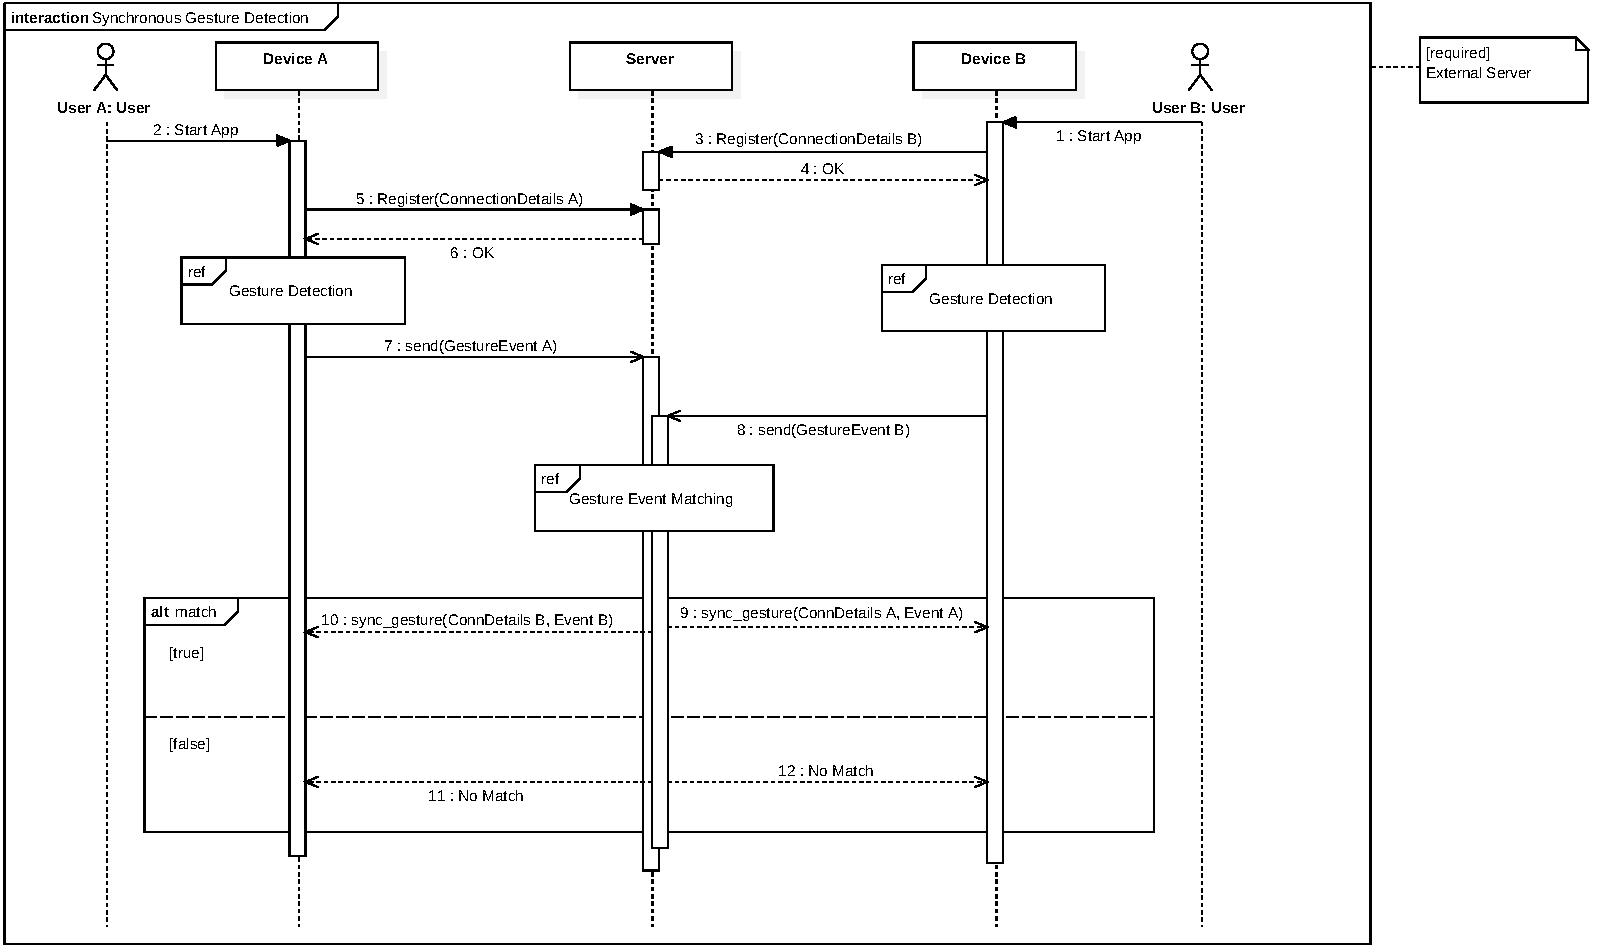
\includegraphics[width=1\textwidth, height=0.65\textheight, keepaspectratio]{bilder/synchronous_gesture_detection.pdf}
\caption{Kommunikationsprotokoll zur Erkennung synchroner Gesten.}
\label{fig:sync_gesture_detection}
\end{sidewaysfigure}

Zwei Geräte (bezeichnet als Gerät A und B) verbinden sich mit einem externen Server, der im Netzwerk erreichbar ist, Nachrichten verschicken und empfangen oder Programmlogik ausführen kann. Auf beiden Geräten wird zunächst eine einfache Gestenerkennung durchgeführt, hier als Referenz auf die in Kapitel \ref{subsec:simple_gesture} beschriebene einfache Gestenerkennung. Die resultierenden \textit{GestureEvents} werden anschließend von beiden Geräten an den Server gesendet, der einen Vergleich aller eingehenden Events durchführt. Wird ein erfolgreicher Vergleich zweier Events vorgenommen, also eine synchrone Geste erkannt, informiert der Server die beteiligten Geräte über die Verbindungsparameter (\textit{ConnectionDetails}) ihrer jeweiligen Kommunikationspartner.

Abbildung \ref{fig:gesture_event_matching} zeigt eine Blackbox-Sicht auf die Aktivität \textit{Gesture Event Matching}, welche den Vergleich von zwei \textit{GestureEvents} vornimmt. Zwei beliebige Events, \textit{Event A} und \textit{Event B}, werden als Eingabe akzeptiert. Innerhalb der Aktivität wird ein Vergleich der Event-Parameter durchgeführt, der analog zur einfachen Gestenerkennung einen Wahrheitswert zurückgibt. Besteht zwischen den beiden Events ein Zusammenhang, bilden sie zusammen eine synchrone Geste.
\begin{figure}[h]
\centering
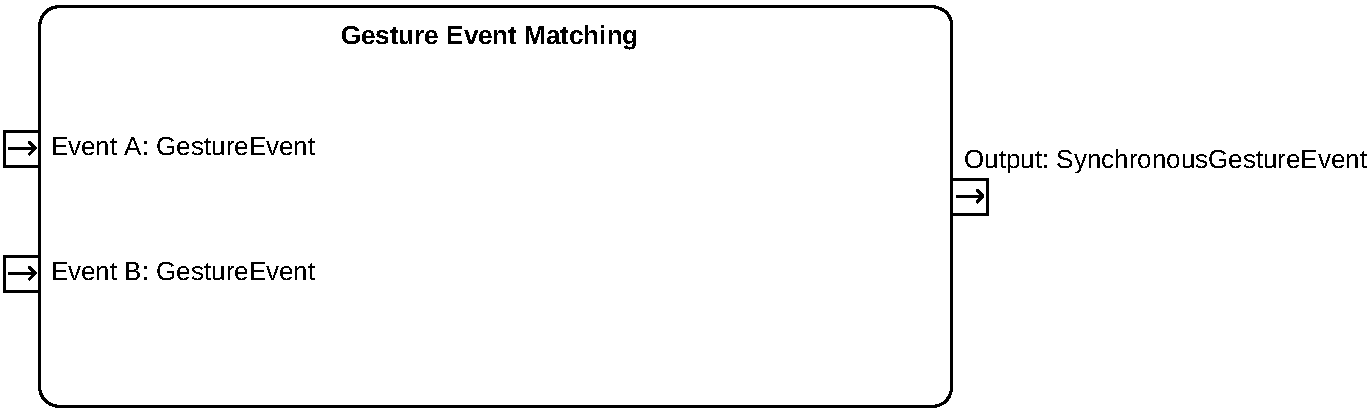
\includegraphics[width=0.7\textwidth]{bilder/gesture_event_matching.pdf}
\caption{Vergleich von \textit{GestureEvents} zur Erkennung synchroner Gesten.}
\label{fig:gesture_event_matching}
\end{figure}

\begin{figure}[h]
\centering
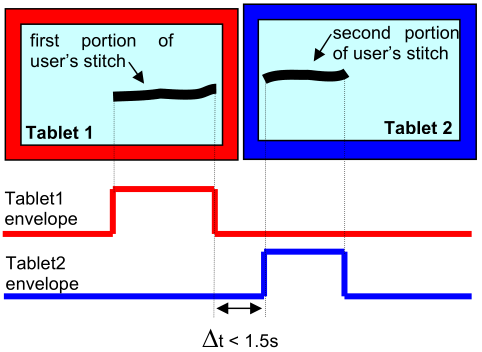
\includegraphics[width=0.5\textwidth]{bilder/stitch_details.png}
\caption{Zusammenhang zwischen Swipe-Events und Stitch-Erkennung. Quelle: \citep{Hinckley2004}.}
\label{fig:stitch_details}
\end{figure}

Ein detailliertes Beispiel für die Erkennung einer synchronen Geste liefern Hinckley und Kollegen mit der Beschreibung der Stitch-Geste (s. auch Kapitel \ref{subsec:model_overview}) \citep{Hinckley2004}. Zunächst wird pro Gerät ein Swipe erkannt, der gewissen Constraints unterliegt. So müssen die Swipes eine zeitliche Mindestlänge und eine bestimmte Richtung aufweisen. Bis dahin handelt es sich um einfache Gesten. Eine exemplarische Beschreibung solcher Swipe-Gesten durch das Modell wurde bereits in Kapitel \ref{subsec:simple_gesture} vorgenommen. Anschließend wird ein Vergleich definiert, ob die jeweiligen Swipes (vgl. Abbildung \ref{fig:stitch_details})
\begin{itemize}
\item eine durchgehende Linie bilden, also ob beide Swipe-Gesten die gleiche Richtung haben,
\item beide Swipe-Gesten mit einem zeitlichen Abstand von \(t<\SI{1.5}{\second}\) ausgeführt wurden und
\item der Austrittswinkel \(\alpha_1\) auf Tablet 1 gleich dem Eintrittswinkel \(\alpha_2\) auf Tablet 2 ist, mit einer Toleranz von \(\pm \ang{20}\).
\end{itemize}

Dazu wird im Modell ein \textit{Stitch Event Matching} definiert, das zwei \textit{SwipeEvents} als Eingabeparameter hat und einen Wahrheitswert zurückgibt, ob eine synchrone Geste erkannt wurde. Abbildung \ref{fig:stitch_event_matching} zeigt die Modellierung dieses Vergleichs. Ein Aktivitätsdiagramm beschreibt die Abfolge der Prüfungen. Durch Annotationen können einfache Vergleiche oder Berechnungen komplexerer Parameter auf Basis der \textit{SwipeEvent}-Parameter definiert werden. In diesem Fall werden die oben beschriebenen Werte Richtung, Zeitdifferenz und Ein- bzw. Austrittswinkel der Swipes berücksichtigt. Setzt man in dem Modell in Abbildung \ref{fig:sync_gesture_detection} für die \textit{Gesture  Detection} eine Swipe-Erkennung wie in Kapitel \ref{subsec:simple_gesture} und für das \textit{Gesture Event Matching} das Stitch Event Matching ein, erhält man eine vollständig beschriebene, synchrone Geste.
\begin{figure}[h]
\centering
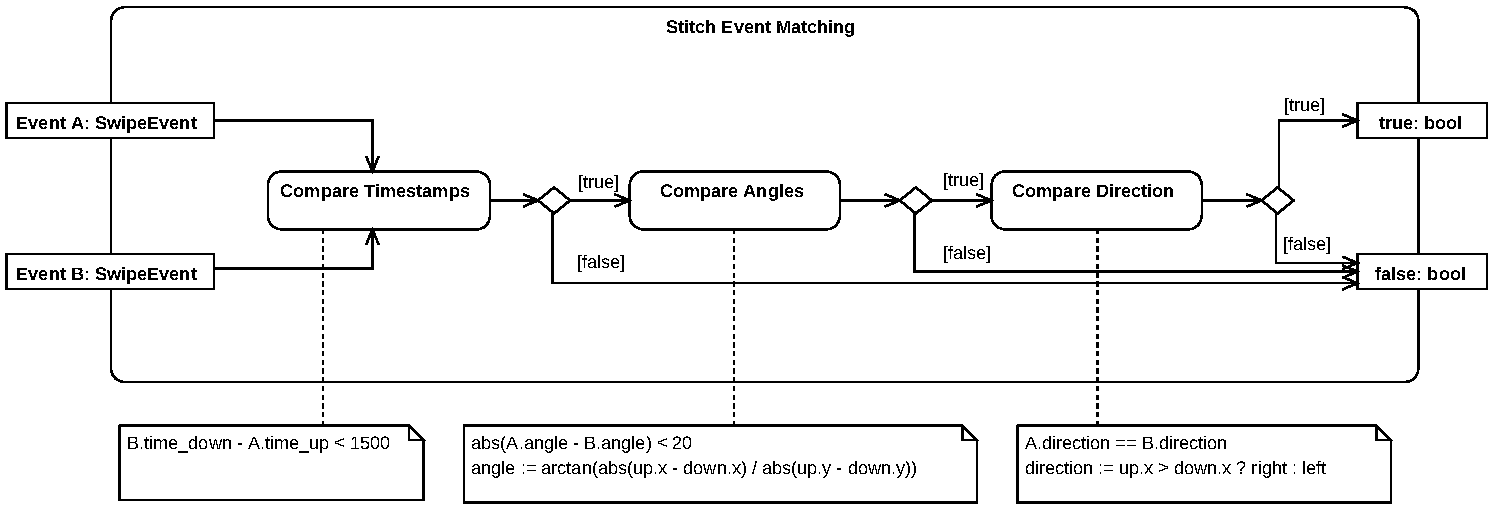
\includegraphics[width=1\textwidth]{bilder/stitch_event_matching.pdf}
\caption{Vergleich zweier Swipe-Events zur Erkennung der synchronen Stitch-Geste.}
\label{fig:stitch_event_matching}
\end{figure}

Hinckley stellt mit der Bump-Geste eine weitere synchrone Geste im Detail vor \citep{Hinckley2003}. Zwei Geräte (bezeichnet als \textit{lokales} und \textit{entferntes} Gerät), die über einen Beschleunigungssensor verfügen, überwachen dabei kontinuierlich ihre Beschleunigung. Ein Bump wird zunächst je Gerät über eine Spitze (engl. \textit{peak}) in der Beschleunigungskurve erkannt (siehe Abbildung \ref{fig:bump_details}). Eine Spitze liegt vor, wenn eine vordefinierte Schwelle über- und anschließend wieder unterschritten wird, sofern dies in einem Zeitfenster von maximal \SI{65}{\milli\second} passiert. Im resultierenden \textit{BumpEvent} wird der Zeitpunkt sowie die Richtung der maximalen Beschleunigung innerhalb der Spitze notiert. Dieser Vorgang kann soweit als einfache Geste beschrieben werden (vgl. Kapitel \ref{subsec:simple_gesture}). Anschließend wird das lokale \textit{BumpEvent} mit denen eines entfernten Gerätes verglichen, zu dem eine Netzwerkverbindung besteht. Gab es auf dem entfernten Gerät eine Spitze, deren Zeitstempel maximal \SI{50}{\milli\second} von der lokalen Spitze entfernt und deren Richtung entgegengesetzt ist (vgl. Abbildung \ref{fig:bump_details}), wird die synchrone Geste erkannt und beide Geräte über ihren Kommunikationspartner informiert.
\begin{figure}[h]
\centering
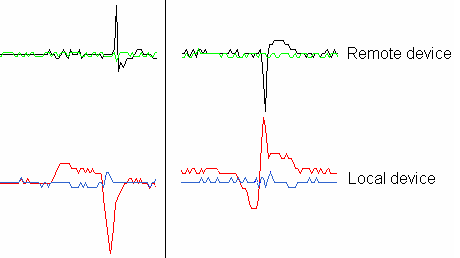
\includegraphics[width=0.7\textwidth]{bilder/bump_accel.png}
\caption{Typische Beschleunigungsmuster der Bump-Geste. Quelle: \citep{Hinckley2003}.}
\label{fig:bump_details}
\end{figure}

Auch die Bump-Geste lässt sich analog zum Stitch durch das Modell beschreiben. Es müssen entsprechend dem Modell in Abbildung \ref{fig:sync_gesture_detection} folgende Komponenten spezifiziert werden:
\begin{itemize}
\item Eine einfache \textit{Bump Detection}, die Werte eines Beschleunigungssensors pro Gerät überwacht, auf Spitzen reagiert und ein \textit{BumpEvent} erzeugt.
\item Ein \textit{Bump Event Matching}, das je zwei \textit{BumpEvents} entgegennimmt, Richtung und Zeitpunkt der Maximalbeschleunigungen vergleicht und einen Wahrheitswert zurückgibt, ob eine synchrone Geste vorliegt oder nicht.
\end{itemize}

Ein weiteres Beispiel für synchrone Gesten findet sich in \citep{Rekimoto2004}. Hier wird das synchrone Drücken und Loslassen von Buttons erkannt. Wurde auf beiden Geräten ein Knopf gleich lange gedrückt (mit einer Toleranz \(c_1=\SI{100}{\milli\second}\)) und zum gleichen Zeitpunkt wieder losgelassen (mit einer Toleranz \(c_2=\SI{200}{\milli\second}\)), wird eine synchrone Geste erkannt (siehe Abbildung \ref{fig:sync_tap}). Spezifiziert werden müssen auch hier:
\begin{itemize}
\item Eine \textit{Gesture Detection}, die \textit{ButtonEvents} erzeugt.
\item Ein \textit{Gesture Event Matching}, das Länge und Zeitpunkte der \textit{ButtonEvents} unter Einbeziehung von \(c_1\) und \(c_2\) vergleicht.
\end{itemize}

\begin{figure}[h]
\centering
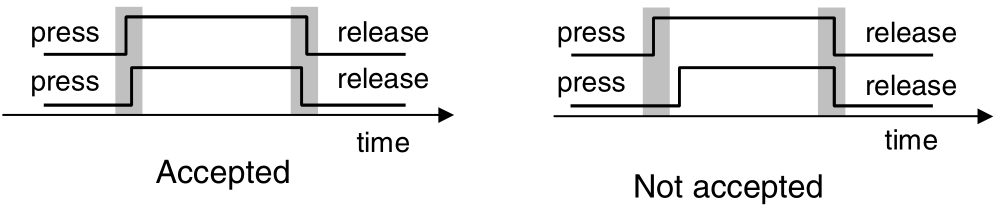
\includegraphics[width=1\textwidth]{bilder/sync_tap.png}
\caption{Erkennung einer synchronen Geste basierend auf Buttons im System SyncTap. Quelle: \citep{Rekimoto2004}.}
\label{fig:sync_tap}
\end{figure}

Eine Ergänzung muss an dieser Stelle noch vorgenommen werden. Das Modell in Abbildung \ref{fig:sync_gesture_detection} geht vom einfachsten Fall aus, in dem ein Server zwischen den einzelnen Geräten vermittelt. Dadurch können auch Geräte miteinander verbunden werden, die sich vorher nicht kennen. In \citep{Hinckley2004} wird eine Infrastruktur vorgestellt, in der ein Gerät selbst die Rolle des Servers übernimmt und dessen Adresse allen anderen Geräten bekannt sein muss. In dem Fall wird keine zusätzliche Vermittlungskomponente benötigt, ebenso wenn zwei Geräte bereits per Ad-hoc-Netzwerk miteinander verbunden sind und somit unmittelbar eine synchrone Gestenerkennung durchführen können.

In \citep{Rekimoto2004} wird zudem eine Alternative beschrieben, in der sich alle Geräte in einem gemeinsamen LAN bzw. WLAN befinden und UDP\footnote{Das \ac{UDP} ist ein simples, verbindungsloses Netzwerkprotokoll, um Pakete in einem Netzwerk zu versenden und zu empfangen. UDP wird oft eingesetzt, wenn Paketverluste akzeptabel sind oder die Reihenfolge des Eintreffens von gesendeten Paketen keine Rolle spielt.}-Pakete mit Button-Events an alle SyncTap-Netzwerkteilnehmer versenden (Multicast). Das \textit{Gesture Event Matching} wird in dem Fall auf jedem Gerät parallel ausgeführt, anstatt nur auf einem dedizierten Gerät. Für beide Fälle muss das Modell aus \ref{fig:sync_gesture_detection} leicht abgewandelt werden, die Ergänzungen befinden sich in Anhang \ref{a:sync_gestures}.

Im folgenden Kapitel wird beschrieben, wie der Verbindungsaufbau zwischen Geräten im Allgemeinen gestaltet werden und wie die Erkennung einfacher oder synchroner Gesten in diesen Ablauf eingebettet werden kann.

\subsection{Connect}
\label{subsec:connect}
Das Rahmenmodell in Kapitel \ref{subsec:model_overview} sieht im Lebenszyklus von \msas zunächst das Verbinden zweier Geräte in Form der Aktivität 
\textit{Connect} vor, deren Details in diesem Kapitel beschrieben werden.

In der SysPlace-Patternsammlung finden sich unter der Kategorie \textit{Connect} verschiedene Patterns zum Aufbauen einer Verbindung zwischen zwei Geräten, die alle auf einer (zumeist synchronen) Geste basieren, wie \zb der Bump- und Stitch-Geste oder dem gleichzeitigen Schütteln zweier Geräte. Wurde die synchrone Geste erkannt, wird auf beiden Geräten gleichzeitig eine Systemreaktion ausgelöst, die den Verbindungsaufbau zwischen diesen Geräten zum Ziel hat. Abbildung \ref{fig:sync_connect} zeigt im Detail, welche Aktivitäten und System-Feedbacks dabei auf beiden Geräten ausgeführt werden und wie sie in Beziehung zueinander stehen. Dazu wird ein Aktivitätsdiagramm verwendet, das zwischen Aktivitäten (pro Gerät) und Events unterscheidet, die entweder die Kommunikation zwischen den Geräten bzw. eventuelle Fehlerfälle darstellen.
\begin{sidewaysfigure}
\centering
\includegraphics[page=2, width=\textwidth]{bilder/connect.pdf}
\caption{Aufbauen einer Verbindung zwischen zwei Geräten mittels synchroner Geste.}
\label{fig:sync_connect}
\end{sidewaysfigure}

Angestoßen wird die \textit{Connect}-Aktivität, wenn eine synchrone Geste erkannt wurde. Kapitel \ref{subsec:simple_gesture} und \ref{subsec:synchronous_gesture} beschreiben die Modellierung der Gestenerkennung ausführlich, in diesem Diagramm wird lediglich eine Blackbox-Sicht verwendet. Dadurch wird die Geste komplett austauschbar, da für den weiteren Verbindungsaufbau lediglich die Parameter für die Verbindung, wie \zb Geräteadressen, in Form von \textit{ConnectionDetails} bekannt sein müssen. 

Sobald die Kommunikationspartner über die \textit{ConnectionDetails} informiert sind, akzeptiert eines der Geräte eingehende Verbindungen, während das andere Gerät versucht, sich mit diesem zu verbinden. Kann die Verbindung erfolgreich hergestellt werden, ist das Ergebnis ein bidirektionaler Datenkanal (\textit{Channel}), über den beide Geräte Nachrichten austauschen können, die Aktivität \textit{Connect} wird dann erfolgreich beendet. Kommt es zu einem Fehler beim Verbindungsaufbau, endet die gesamte Aktivität auf beiden Geräten ohne Verbindung.

Die Nutzer beider Geräte erhalten an verschiedenen Stellen jeweils ein \textit{Feedback} des Systems, ob die Verbindung aufgebaut werden konnte oder nicht (siehe orangene Aktivitäten in Abbildung \ref{fig:sync_connect}, die mit \textit{Feedback} gekennzeichnet sind). Solche Feedback-Aktivitäten sind lediglich Design-Hinweise, dass es an dieser Stelle sinnvoll sein kann, den Nutzer über den Systemzustand zu informieren. Wie die Rückmeldung gestaltet wird, muss für jede Anwendung individuell entschieden werden. Gestaltungsmöglichkeiten entsprechend den Ausgabetechnologien aus Kapitel \ref{subsec:ausgabe} sind u.a.:
\begin{itemize}
\item \textit{visuelles Feedback}: Veränderungen in der Nutzeroberfläche, wie \zb Einblendung von Textboxen, Animationen oder Ändern der Farbe.
\item \textit{akustisches Feedback}: Abspielen von Geräuschen, um den Nutzer über Veränderungen zu informieren und evt. visuelles Feedback zu unterstützen.
\item \textit{Vibration}: Mobile Geräte können Vibrationen erzeugen, um den Anwender über Änderungen zu informieren.
\end{itemize}
Da System-Feedback beliebig gestaltet und kombiniert werden kann, ist eine modellhafte Erfassung an dieser Stelle nur eingeschränkt sinnvoll. Es ist lediglich möglich, die benötigten Ausgabetechnologien zu erfassen, die für eine bestimmte Ausgestaltung des Feedbacks mindestens benötigt werden. Dazu wird in Kapitel \ref{subsec:domain_model} beschrieben, wie System-Feedback unter Einbeziehung benötigter Ausgabetechnologien statisch durch das Modell erfasst werden kann.

In der Literatur finden sich vielerlei Hinweise für die Gestaltung des Verbindungsprozesses sowie des Feedbacks. Einige Beispiele, die bei der Erstellung des Modells berücksichtigt wurden, werden im Folgenden dargestellt.

Hinckley schlägt für die Verwendung der Bump-Geste zum Verbindungsaufbau verschiedene Feedback-Mechanismen vor \citep{Hinckley2003}:
\begin{itemize}
\item Ein kurzes, metallisches Klicken auf dem Tablet, welches die Geste erkannt hat, um ein "`Zusammenschnappen"' der Tablets anzudeuten (\textit{akustisches Feedback}).
\item Einen Pfeil zum Bildschirmrand, der andeutet, dass eine Verbindung mit einem anderen Tablet aufgebaut wird (\textit{visuelles Feedback}).
\item Einen "`popping sound"', der auf dem zweiten Tablet abgespielt wird, wenn der Verbindungsaufbau erfolgreich abgeschlossen wurde (\textit{akustisches Feedback}).
\item Einen zweiten, kleineren Pfeil zum Bildschirmrand des zweiten Tablets, der mit dem ersten Pfeil zusammen nach zwei Sekunden wieder ausgeblendet wird (\textit{visuelles Feedback}).
\end{itemize}

Hinckley betont, dass es wichtig sei, visuelles und akustisches Feedback zu kombinieren, falls ein Nutzer \zb gerade nicht seinen Fokus auf den Tablets hat und eine Verbindung zustande gekommen ist. 

Ferner merkt er an, dass das Feedback auf beiden Geräten zwar oft simultan und redundant stattfindet, es aber dennoch in jedem Fall stattfinden solle, falls der Verbindungsaufbau bspw. länger dauert und der Nutzer sonst nicht weiß, ab wann eine Verbindung besteht. Die Geräte werden  über WLAN miteinander verbunden, als Netzwerkprotokoll wird \acs{TCP}\footnote{Das \ac{TCP} ist ein verbindungsorientiertes Netzwerkprotokoll, in dem im Gegensatz zu \acs{UDP} verlorene Pakete neu gesendet werden und die Reihenfolge gesendeter Pakete beachtet wird.} eingesetzt \citep{Hinckley2003}.

Das Modell in Abbildung \ref{fig:sync_connect} ermöglicht es, diese Design-Hinweise zu berücksichtigten. So können das akustische Feedback (metallisches Klicken) sowie der visuelle Hinweis (der Pfeil) als \textit{Feedback Start} auf dem Tablet eingeblendet werden, das auf eingehende Verbindungen wartet. Sobald das zweite Tablet sich verbunden hat, kann auf diesem der zweite Sound sowie der entgegengesetzte Pfeil als \textit{Feedback Success} eingeblendet werden. Zudem werden nach zwei Sekunden beide Pfeile ausgeblendet, was ebenfalls unter \textit{Feedback Success} auf beiden Tablets berücksichtigt werden muss. Hinckley definiert für den Fall, dass keine Verbindung zustande kommt, kein explizites Feedback \citep{Hinckley2003}. Auf dem Tablet, das auf eingehende Verbindungen wartet, muss dann zwar als \textit{Feedback Error} der Pfeil ausgeblendet werden, für das andere Tablet würde aber kein \textit{Feedback Error} definiert. 

Auch das verwendete Netzwerkprotokoll TCP findet sich vereinfacht in dem Modell wieder (Akzeptieren von Verbindungen auf Gerät A bzw. aktives Verbinden von Gerät B zu Gerät A). Weitere Details werden hier bewusst ausgelassen, da der Verbindungsaufbau der meisten Netzwerktechnologien nach einem ähnlichen Schema funktioniert und eine detaillierte Beschreibung das Modell unnötig verkomplizieren würde.

Für die Stitch-Geste finden sich ebenfalls Designhinweise bzgl. der \textit{Connect}"=Aktivität, die sich durch das Modell beschreiben lassen \citep{Hinckley2004}. So definieren Hinckley und Kollegen, dass ein kurzer Piepton abgespielt wird, sobald die Stitch-Geste auf dem zweiten Tablet erkannt wird (siehe Abbildung \ref{fig:stitch_details}). Zudem können eventuell zu übertragene Daten auf dem ersten Tablet visuell hervorgehoben werden. Hierfür wird keine bestehende Verbindung benötigt, beides kann als \textit{Feedback Start} definiert werden. Hinckley beschreibt zudem, dass bei erfolgreicher Verbindung ein Menü eingeblendet wird, welches dem Nutzer Operationen auf den selektierten Daten vom ersten Tablet anbietet (\zb Kopieren der Daten auf das zweite Tablet). Das ist erst sinnvoll, wenn bereits eine Verbindung besteht, also in der Aktivität \textit{Feedback Success}. Das Menü geht über beide Bildschirme (siehe Abbildung \ref{fig:stitch_menu}) und muss dementsprechend für beide Geräte definiert werden.
\begin{figure}[h]
\centering
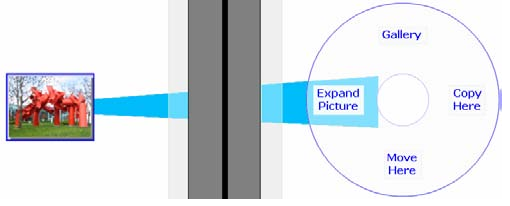
\includegraphics[width=0.7\textwidth]{bilder/stitch_menu.png}
\caption{Optionsmenü als visuelles Feedback nach erfolgreicher Stitch-Geste. Quelle: \citep{Hinckley2004}.}
\label{fig:stitch_menu}
\end{figure}

Anzumerken ist, dass beim Stitch meist die Rahmenmodell-Variante aus Abbildung \ref{fig:model_overview_alternative} zum Einsatz kommt, da teilweise vor dem Verbinden von Geräten schon Daten selektiert werden. Als Netzwerktechnologie kommt WLAN zum Einsatz. Es wird kein Netzwerkprotokoll explizit erwähnt, vermutlich wird aber analog zur Bump-Geste in \citep{Hinckley2003} wieder \acs{TCP} verwendet.

Zwar werden meist synchrone Gesten zum Aufbauen einer Verbindung verwendet, allerdings sind auch einfache Gesten auf einem Gerät denkbar, um den Verbindungsaufbau einseitig anzustoßen. Abbildung \ref{fig:async_connect} zeigt eine Abwandlung des Modells, das auf einfachen Gesten basiert. In diesem Fall führt nur der Nutzer von Gerät A eine Geste aus, durch die ein Verbindungsaufbau zu Gerät B initiiert wird. Der Nutzer von Gerät B muss die Möglichkeit haben, die Verbindung entweder anzunehmen oder abzulehnen, was durch eine Aktivität vom Typ \textit{User Interaction} berücksichtigt wurde, die analog zum Feedback individuell an die Applikation angepasst werden kann.
\begin{sidewaysfigure}
\centering
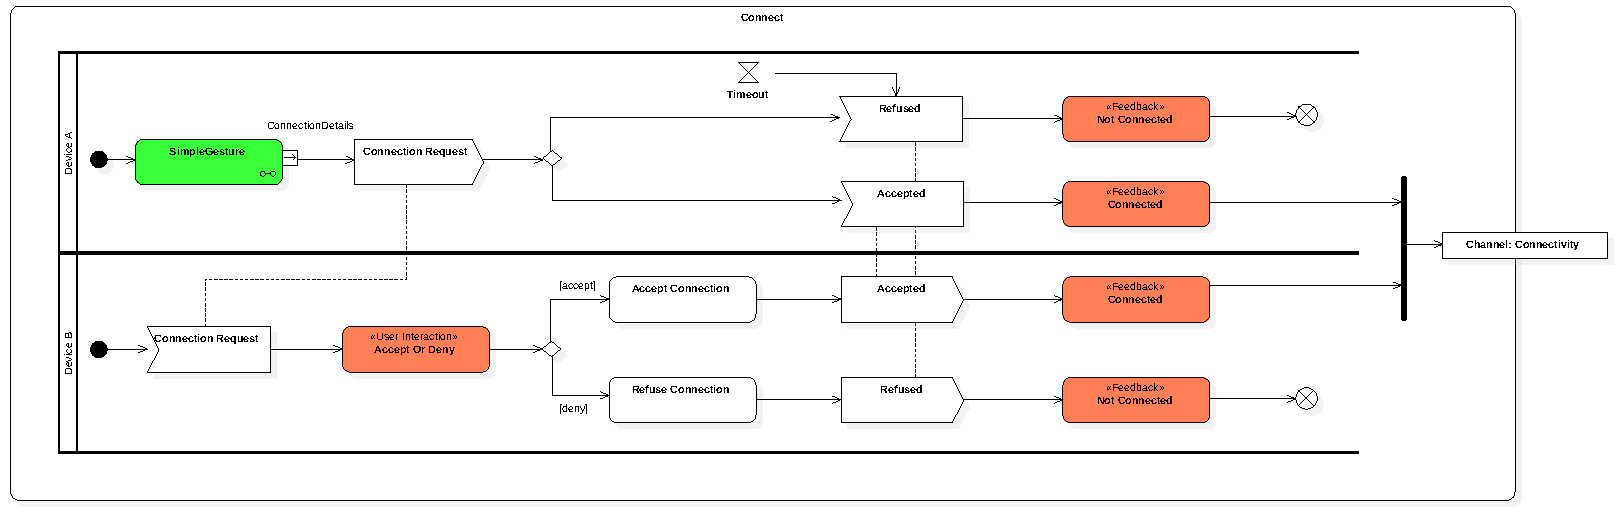
\includegraphics[page=1, width=\textwidth]{bilder/connect.pdf}
\caption{Aufbauen einer Verbindung zwischen zwei Geräten mittels einfacher Geste.}
\label{fig:async_connect}
\end{sidewaysfigure}

Eine interessante Anwendung dazu findet sich im System BlueTable \citep{Wilson2007}. Hier soll die exakte Position von mobilen, Bluetooth-fähigen Geräten auf einer interaktiven Oberfläche\footnote{Mit interaktiver Oberfläche ist hier ein System gemeint, das Berührungen oder physikalische Objekte auf einer Fläche erkennen und tracken kann. In \citep{Wilson2007} wird dazu das System Play"=Anywhere verwendet, das aus einem Projektor und einer Kamera besteht und normale Oberflächen digital erfassen kann (eine ausführliche Beschreibung von PlayAnywhere findet sich in \citep{Wilson2005}).} erkannt werden, ohne auf Technologien wie \acs{RFID} oder \ac{NFC} zurückzugreifen. Dazu schlagen die Autoren folgenden Ablauf vor:
\begin{enumerate}
\item Die interaktive Oberfläche erkennt, dass ein Smartphone-förmiges Objekt an einer bestimmten Position aufgelegt wurde.
\item Das System baut zu jedem Bluetooth-fähigen Gerät in Reichweite eine Verbindung auf, sofern dieses eine vordefinierte BlueTable-Service-ID aussendet.
\item Sobald eine Verbindung besteht, wird das Gerät aufgefordert, seinen Infrarot-Port aufblinken zu lassen.
\item Stimmt die Position des Blinkens mit der Position des Auflegens überein, besteht eine Bluetooth-Verbindung zu dem Smartphone an exakt dieser Position.
\end{enumerate}

Definiert man das Auflegen eines Smartphones als Geste auf der interaktiven Oberfläche, kann man dieses System durch das Modell in Abbildung \ref{fig:async_connect} beschreiben. Gerät A (die interaktive Oberfläche) erkennt das Auflegen eines Gerätes B und sendet eine Bluetooth-Anfrage an alle Bluetooth-Geräte in Reichweite. Erhält ein beliebiges Gerät diese Anfrage, kann die Verbindung akzeptiert oder abgelehnt werden. Dazu wird analog zu Feedback-Aktivitäten eine Aktivität vom Typ \textit{User Interaction} eingeführt, die je nach Anwendungskontext individuell gestaltet werden muss. Die Option, die Verbindung abzulehnen, ist für alle Geräte sinnvoll, die außer Gerät B die Anfrage erhalten, weil sie zwar in Bluetooth-Reichweite sind, aber nicht aufgelegt wurden.

Akzeptiert ein Gerät die Verbindungsanfrage, ergibt sich hier als Besonderheit, dass das \textit{Feedback Connected} neben eventuellen anderen Ausgaben das Blinken der Infrarot-Lampe beinhaltet und somit die Positionsbestimmung ermöglicht. Haben mehrere Geräte die Verbindung akzeptiert und ein Infrarot-Blinken ausgelöst, hält Gerät A die Verbindung nur zu demjenigen Gerät, dessen Position mit der Auflegeposition übereinstimmt, also Gerät B.

Dieser Bluetooth-Kanal wird anschließend für die weitere Applikationslogik genutzt, um \zb Kontaktinformationen oder Bilder auszutauschen \citep{Wilson2007}, was nach dem Rahmenmodell (siehe Kapitel \ref{subsec:model_overview}) in den Aktivitäten \textit{Select} bzw. \textit{Transfer} passiert, welche in den folgenden Kapiteln näher beschrieben und modelliert werden.

\subsection{Select}
\label{sec:select}
Um Multiscreen-Szenarien zu realisieren, müssen Daten zwischen Geräten ausgetauscht werden. Diese werden entweder implizit durch den Kontext oder explizit durch den Nutzer ausgewählt, bevor die Übertragung stattfinden kann. Das Rahmenmodell in Kapitel \ref{subsec:model_overview} sieht dazu die Aktivität \textit{Select} vor, die entweder vor (siehe Abbildung \ref{fig:model_overview_alternative}) oder nach der \textit{Connect}-Aktivität (siehe Abbildung \ref{fig:model_overview}) stattfindet, in jedem Fall aber dem \textit{Transfer} von Daten vorausgeht. Auch eine wiederholte Ausführung der \textit{Select}-Aktivität ist möglich, wenn mehrfach Daten übertragen werden sollen. Die Art der selektierten Daten entscheidet darüber, wie der anschließende Übertragungsprozess, also die Aktivität \textit{Transfer}, gestaltet werden kann.

Da das Format von Daten und damit die Gestaltung des Selektionsprozesses stark vom jeweiligen Anwendungskontext abhängt, ist eine Modellierung der \textit{Select}"=Aktivität nur eingeschränkt möglich. Schwierig ist dabei die Erfassung des "`Wie"', also in welcher Art und Weise die Interaktion des Nutzers mit dem System gestaltet wird. Zwar können hier auch Gesten zum Einsatz kommen, die mittels des Modells erfasst werden können (siehe Kapitel \ref{subsec:simple_gesture}), für die Gestaltung der Oberflächen und der Interaktionsformen für die Selektion wird hier allerdings kein allgemeingültiges Modell aufgestellt. Das hat den Grund, dass Oberflächen stark an einen Anwendungskontext sowie die verwendete Plattform gebunden sind und die einheitliche, abstrakte Beschreibung von Nutzeroberflächen ein komplexes Thema ist, das im Rahmen dieser Arbeit nicht berücksichtigt werden kann. Erfasst werden kann aber das "`Was"', also welcher Art die selektierten Daten sind. Abbildung \ref{fig:select} zeigt den Ablauf der Aktivität.
\begin{figure}[h]
\centering
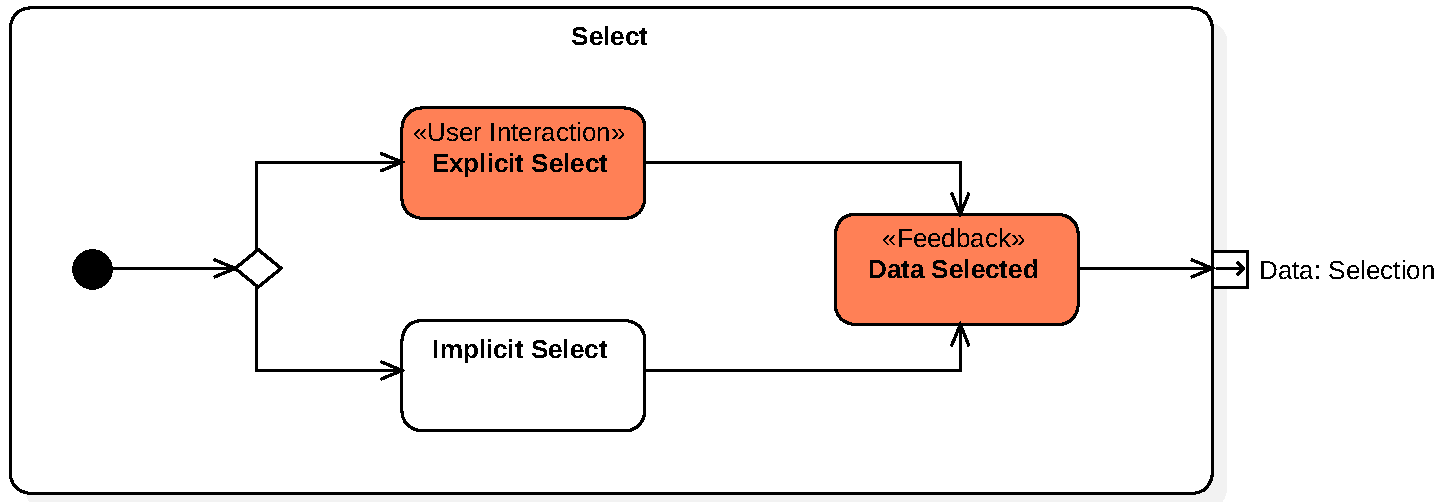
\includegraphics[width=1\textwidth]{bilder/select.pdf}
\caption{Ablauf der Aktivität \textit{Select}.}
\label{fig:select}
\end{figure}

Hier sind die beiden Fälle der impliziten Auswahl durch die Anwendung bzw. der expliziten Auswahl durch den Benutzer (in Form einer Aktivität vom Typ \textit{User Interaction}) berücksichtigt. Zudem kann ein zusätzliches System-Feedback ausgeführt werden, um den Nutzer über die erfolgte Auswahl zu informieren. Das Ergebnis der \textit{Select}-Aktivität ist eine Auswahl (\textit{Selection}) von Daten, deren Typ je nach Kontext variieren kann. Für das Modell wurden vier verschiedene Typen herausgearbeitet:
\begin{itemize}
\item \textit{File}: genau eine Datei, \zb ein Foto oder Textdokument.
\item \textit{MultipleFiles}: eine Menge einzelner Dateien, \zb alle Fotos in einem Ordner.
\item \textit{Stream}: ein Datenstrom (\zb Videodaten), der kontinuierlich übertragen werden soll.
\item \textit{Command}: ein anwendungsspezifischer Steuerbefehl für die entfernte Anwendung.
\end{itemize}

Im System StitchMaster wird eine Selektion einzelner Dateien bzw. einer Menge von Dateien (meist Fotos) implementiert \citep{Hinckley2004}. Der Nutzer kann entweder ein einzelnes Foto (durch Antippen) oder eine Menge von Fotos (mittels einer Lasso-Geste) auswählen, was nach dem Modell in Abbildung \ref{fig:select} einer \textit{expliziten Selektion} eines einzelnen Fotos (\textit{File}) bzw. mehrerer Fotos (\textit{MultipleFiles}) entspricht. Bei der Lasso-Geste wird ein Bereich mit Bildern markiert, dessen Inhalt dann die \textit{Selection} bildet (siehe Abbildung \ref{fig:stitch_select} (a)). Die Beschreibungen der Gesten sind Teil der \textit{User Interaction}.

Um den Benutzer zu informieren, welche Dateien zur Übertragung ausgewählt wurden, werden die Fotos anschließend mit einem Rahmen versehen (siehe Abbildung \ref{fig:stitch_select} (b)), was als visuelles Feedback \textit{Data Selected} im Modell berücksichtigt werden kann. Als Ergebnis der Aktivität wird die \textit{Selection} des entsprechenden Typs an die Transfer-Aktivität übergeben.
\begin{figure}[h]
\centering
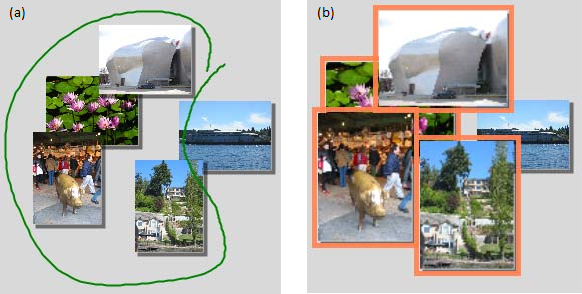
\includegraphics[width=0.7\textwidth]{bilder/stitch_select.png}
\caption{Auswahl mehrerer Dateien im System StitchMaster. (a) Auswahl der Dateien mittels Lasso-Geste. (b) Hervorhebung der Auswahl durch das System. Quelle: \citep{Hinckley2004}.}
\label{fig:stitch_select}
\end{figure}

Auch in \citep{Hinckley2003} werden verschiedene Gestaltungsmöglichkeiten des Selektionsvorgangs besprochen, die der Übertragung mittels Bump-Geste vorausgehen können. So wählt der Benutzer im einfachsten Fall explizit ein Foto (\textit{File}) aus, das auf dem anderen Bildschirm angezeigt werden soll. Dabei wird nach der Übertragung entweder eine Kopie angezeigt, oder das Bild wird auf beide Bildschirme aufgeteilt (sog. \textit{Display Tiling}). In diesem Fall müssen noch zusätzliche \textit{Commands} übergeben werden, um \zb die Bildschirmgröße zu übermitteln, damit beide Geräte ihren jeweiligen Teilausschnitt des Bildes berechnen können. Diese \textit{Commands} werden implizit durch die Anwendung ermittelt, es findet keine weitere Nutzerinteraktion statt.

Auch eine sog. \textit{Face-to-face Collaboration} wird beschrieben, bei der Benutzer ein geteiltes Whiteboard auf beiden Geräten benutzen können. In dem Fall wäre die \textit{Selection} vom Typ \textit{Stream}, da kontinuierlich Eingaben auf beiden Whiteboards synchronisiert werden müssen.

Ein weiterer Anwendungsfall ist das Teilen einer betrachteten Webseite. Ist auf einem Gerät eine Webseite geöffnet und es wird eine Bump-Geste ausgeführt, soll auf dem zweiten Gerät der Browser geöffnet und die gleiche Seite angezeigt werden \citep{Hinckley2003}. Modelliert werden könnte dies mittels eines \textit{Commands}, der als Parameter die zu startende Applikation (Browser) und den Startparameter (\acs{URL}) übermittelt.

Analog dazu könnte der ebenfalls beschriebene Anwendungsfall erfasst werden, in der ein Word-Dokument geteilt und zur selben Stelle gesprungen werden soll \citep{Hinckley2003}. Hier wären die Parameter die gleichen, nur die Werte für Applikation (Word) und Startparameter (Netzwerkpfad zum Dokument und Seitennummer) wären unterschiedlich. In beiden Fällen ist die Art der Selektion eher impliziter Natur, da der Nutzer nur die Anwendung in einem bestimmten Zustand geöffnet hat und diese automatisch die aktuelle Auswahl in Form eines \textit{Commands} aus diesem Zustand ableitet.

Dachselt und Kollegen gehen ebenfalls auf den Auswahlprozess und die Art der ausgewählten Daten in ihrem Multiscreen-Szenario ein (siehe auch Kapitel \ref{subsec:model_overview} für eine kurze Beschreibung des Systems) \citep{Dachselt2009}. Im ersten Schritt werden alle auf einem Smartphone vorhandenen Fotos implizit selektiert, die mittels der anschließenden Wurf-Geste übertragen werden können. Nach der Übertragung hat der Benutzer die Möglichkeit, die übertragenen Bilder auf dem Smart TV durch Kippen des Smartphones durchzuschalten. Dabei wird mittels einer Tilt-Geste explizit ein \textit{Command} selektiert, der dem Smart TV mitteilt, zum nächsten Foto zu schalten. Zudem können die Bilder durch eine weitere Geste vom Smart TV entfernt werden, was wiederum eine explizite \textit{User Interaction} in Form einer Fetch-Back-Geste ist, aus welcher ein \textit{Command} zum Entfernen der Bilder abgeleitet wird. 

Im Sinne des Applikationslebenszyklus (siehe Kapitel \ref{subsec:model_overview}) ergibt sich in dem Fall also eine mehrfache Ausführung der Aktivität \textit{Select}, wobei je nach Zustand der Applikation entweder Dateien oder eine Folge von Steuerbefehlen übermittelt werden, um das gesamte Multiscreen-Szenario zu realisieren. Jede dieser Ausprägungen der \textit{Select}-Aktivität muss  modelliert werden, wenn die Anwendung komplett abgebildet werden soll.

Im folgenden Kapitel wird der Zusammenhang zwischen einer abgeschlossenen \textit{Select}-Aktivität und dem Auslösen des Transfers beschrieben. Zudem wird ein für alle \textit{Selection}-Typen einheitlicher Transfer-Prozess modelliert.

\subsection{Transfer}
\label{subsec:transfer}
Entsprechend dem Rahmenmodell in Kapitel \ref{subsec:model_overview} findet die  \textit{Transfer}-Aktivität entweder unmittelbar nach den Aktivitäten \textit{Connect} oder \textit{Select} statt, in jedem Fall aber erst dann, wenn beide Aktivitäten einmal ausgeführt wurden und damit zwei Voraussetzungen erfüllt sind:
\begin{itemize}
\item Es besteht eine bidirektionale\footnote{Der Einfachheit halber wird hier immer eine bidirektionale Verbindung angenommen, da die meisten Netzwerktechnologien bidirektional funktionieren und somit keine weitere Unterscheidung zwischen Aktivitäten mit uni- oder bidirektionalem Datenaustausch vorgenommen werden muss.} Verbindung zwischen zwei Geräten (\textit{Channel}).
\item Auf einem Gerät wurden Daten zur Übertragung ausgewählt (\textit{Selection}).
\end{itemize}
\begin{figure}[h]
\centering
\includegraphics[page=2,width=1\textwidth]{bilder/transfer.pdf}
\caption{Beginn des Transfers mit Vorbedingungen und Auslösern.}
\label{fig:transfer}
\end{figure}

Abbildung \ref{fig:transfer} zeigt den Beginn des Transfer-Ablaufes unter Berücksichtigung dieser Voraussetzungen. Erst wenn beide Inputs vorhanden sind, kann ein Transfer durchgeführt werden. Ein Auslöser wird benötigt, um den Transfer der ausgewählten Daten zu starten. Hier gibt es zwei Möglichkeiten:
\begin{itemize}
\item Der Auslöser ist eine einfache oder synchrone Geste oder
\item die Übertragung wird automatisch gestartet, wenn keine explizite Geste mehr erforderlich ist (\zb dann, wenn nur ein \textit{Command} übertragen wird).
\end{itemize}
Sobald beide Voraussetzungen erfüllt sind und einer der Auslöser erkannt wurde,  wird die Datenübertragung in der Aktivität \textit{Transfer Selected Items} durchgeführt. Die Details dieses Ablaufes werden durch das Modell in Abbildung \ref{fig:transfer_selection} näher beschrieben. 

Das sendende Gerät (\textit{Sender}) informiert den Benutzer über den Start der Datenübertragung und fängt an, Daten an den Empfänger (\textit{Receiver}) zu senden. Dieser informiert ebenfalls mit einem System-Feedback über den Start des Empfangs und verarbeitet die eintreffenden Datenpakete (\textit{Chunks}) kontinuierlich. Für jeden erhaltenen \textit{Chunk} gibt es eine Rückmeldung über den Fortschritt (\textit{Feedback Progress}) sowie einen eventuellen Verarbeitungsschritt (\textit{Process Chunk}), wenn \zb ein Datenstrom empfangen wird. Ebenso gibt es auf der Senderseite kontinuierliches Feedback über den Fortschritt.

Sowohl Sender als auch Empfänger ermöglichen einen Abbruch der Übertragung durch den Nutzer (Event \textit{User Abort}) bzw. können einen Fehler oder Abbruch der Übertragung feststellen (Event \textit{Error / Abort}). In beiden Fällen kann ein Feedback über den Abbruch des Transfers stattfinden. Wird die Übertragung hingegen erfolgreich beendet, findet auf dem Empfänger eine Verarbeitung des Endergebnisses statt, in der \zb eine empfangene Datei angezeigt oder ein Befehl ausgeführt wird. Auf der Senderseite ist dagegen nur ein Feedback über den Erfolg des Transfers vorgesehen, da keine zu verarbeitenden Daten anfallen.
\begin{sidewaysfigure}
\centering
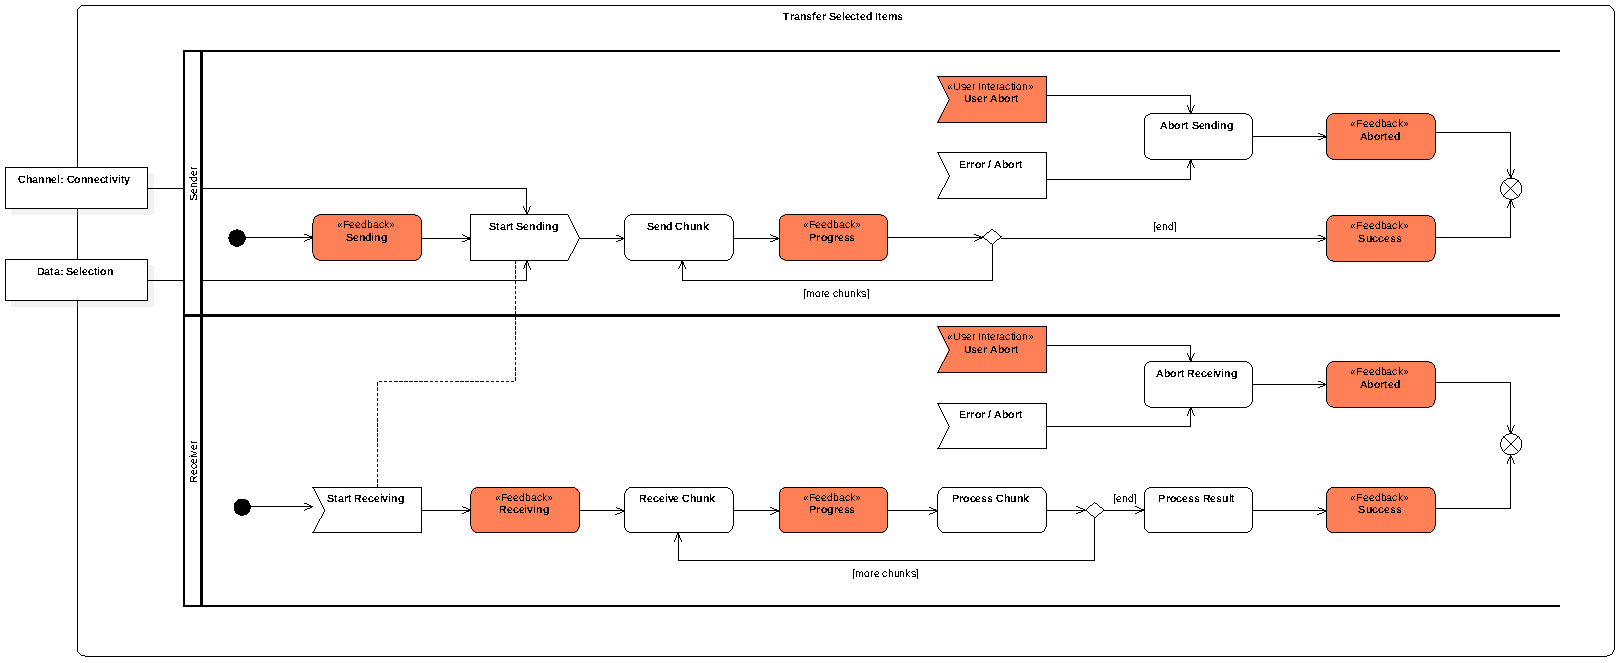
\includegraphics[page=1,width=\textwidth]{bilder/transfer.pdf}
\caption{Ablauf eines Datentransfers in der Aktivität \textit{Transfer Selected Items}.}
\label{fig:transfer_selection}
\end{sidewaysfigure}

Ein Beispiel für die Gestaltung dieses Ablaufes findet sich bei \citep{Hinckley2003}, in dem eine geöffnete Webseite geteilt werden soll. Durch eine Bump-Geste soll die auf einem Gerät geöffnete Webseite auch auf dem anderen Gerät geöffnet werden. Hier sind alle Voraussetzungen zum Start des Transfers erfüllt:
\begin{itemize}
\item Eine (implizite) \textit{Selection} in Form der geöffneten Webseite,
\item eine Verbindung zwischen beiden Geräten (\textit{Channel}), die durch den Bump zustande kommt (siehe Kapitel \ref{subsec:connect}) und
\item die Bump-Geste als Auslöser für die Übertragung.
\end{itemize} 
Hier kommt die Variante aus Abbildung \ref{fig:model_overview_alternative} zum Einsatz, in der die Verbindung und der Transfer durch die gleiche Geste erfolgen. Somit löst die Bump-Geste den Verbindungsaufbau als auch den Transfer aus. Der vorgeschlagene Ablauf des Transfers lässt sich durch das Modell erfassen:
\begin{itemize}
\item Vor dem Transfer wird ein "`Teleportier"'"=Sound abgespielt \citep{Hinckley2003}, zudem werden Pfeile in Richtung der Bildschirmränder angezeigt (\textit{Feedback Starting} / \textit{Feedback Receiving}).
\item Ein \textit{Command} wird übertragen, der die URL der geöffneten Webseite beinhaltet (\textit{Send Chunk} / \textit{Receive Chunk}). In diesem Fall wird die Aktivität \textit{Process Chunk} nicht ausgeführt, da der Befehl erst ausgeführt werden kann, wenn er vollständig übertragen wurde.
\item Der \textit{Receiver} führt den Befehl aus, indem der Browser geöffnet und die Webseite angezeigt wird (\textit{Process Result}).
\end{itemize}

Da das Übertragen eines \textit{Commands} aufgrund des geringen Datenvolumens relativ schnell geht, ist in \citep{Hinckley2003} kein Feedback für Übertragungsprobleme oder Fehlerfälle vorgesehen, es gibt auch kein Feedback über den Fortschritt. Sofern eine Verbindung besteht und die Übertragung gestartet wird, geht Hinckley vermutlich davon aus, dass diese auch erfolgreich beendet werden kann.

Ebenso wird in \citep{Hinckley2003} eine Variante des Systems vorgestellt, in der ein Whiteboard von beiden Nutzern geteilt und gleichzeitig auf beiden Geräten verwendet wird. Auch diese Variante lässt sich mittels des Modells beschreiben:
\begin{itemize}
\item Die \textit{Selection} ist in diesem Fall vom Typ \textit{Stream}.
\item Die Aktivität \textit{Process Chunk} verarbeitet den kontinuierlich eintreffenden Datenstrom.
\item Die Kollaboration wird beendet, wenn ein Benutzer die Verbindung explizit abbricht (\textit{User Abort}) oder den Raum verlässt, wodurch das Event \textit{Error / Abort} ausgelöst wird.
\item Die Aktivität \textit{Process Result} wird nicht benötigt, da nach dem Abbruch der Kollaboration keine abschließende Verarbeitung der Stream-Daten notwendig ist.
\end{itemize}

Auch die Datenübertragungen des Systems von Dachselt und Buchholz (s. auch Kapitel \ref{subsec:model_overview}) können durch das Modell beschrieben werden \citep{Dachselt2009}. Zunächst sollen Bilder durch eine Wurf-Geste vom Smartphone auf das Smart TV übertragen werden. Die drei Bedingungen des Modells in Abbildung \ref{fig:transfer} werden dazu wie folgt definiert:
\begin{itemize}
\item Die \textit{Selection} ist vom Typ \textit{MultipleFiles} und wird implizit erstellt, wenn der Benutzer Fotos in seiner Applikation geöffnet hat.
\item Der \textit{Channel} ist in Form einer Bluetooth- oder Wi-Fi-Verbindung gegeben, die bereits beim Betreten des Raumes aufgebaut wird.
\item Der Auslöser für den Transfer ist eine Wurf-Geste.
\end{itemize}
Für die Übertragung von Daten vom Smart TV auf das Smartphone würde ein ähnlicher Ablauf modelliert. Lediglich Sender und Empfänger wären vertauscht und die Wurf-Geste durch eine Fetch-Back-Geste ersetzt (siehe Kapitel \ref{subsec:model_overview}).

Wird ein Transfer per Wurf-Geste gestartet, werden alle Bilder auf das Smart TV (\textit{Receiver}) übertragen. Dachselt und Buchholz geben hier keine Gestaltungshinweise für den Ablauf der Übertragung, denkbar wäre aber \zb eine Fortschrittsanzeige während des Sendens, da die Menge der gesendeten Bilder bekannt ist. Allerdings finden sich Gestaltungshinweise für den Abschluss des Transfers, den die Anzeige der Bilder als Galerie  in der Aktivität \textit{Process Result} bildet. Auf dem sendenden Smartphone wäre ebenfalls ein \textit{Feedback Success} denkbar.

Zum Durchschalten der Bilder wiederholt sich die \textit{Transfer}-Aktivität, allerdings diesmal in einer anderen Ausprägung:
\begin{itemize}
\item Der \textit{Channel} ist weiterhin verfügbar.
\item Die \textit{Selection} ist vom Typ \textit{Command} ("`Weiterschalten zum nächsten Bild"').
\item Der Auslöser ist \textit{Automatic}, da die Auswahl des Befehls bereits die Geste enthält.
\end{itemize}
Die anschließende Übertragung des Befehls ist ähnlich dem der geteilten Webseite per Bump-Geste. Hier ist weniger Feedback nötig, in der Aktivität \textit{Process Result} wird lediglich das nächste Foto in der Galerie angezeigt.

Es werden so lange \textit{Select}- und \textit{Transfer}-Aktivitäten durchgeführt, bis die Verbindung zwischen Geräten getrennt wird. Sollen keine weiteren Transfers stattfinden, kann die Verbindung entweder aktiv durch den Benutzer oder implizit getrennt werden. Die Modellierung dazu findet sich im folgenden Kapitel.

\subsection{Disconnect}
\label{subsec:disconnect}
Die letzte Aktivität im Lebenszyklus einer Multiscreen-Anwendung ist der \textit{Disconnect}, das Trennen der Verbindung zwischen zwei Geräten (s. Rahmenmodell in Kapitel \ref{subsec:model_overview}). Im Vergleich zum Verbindungsaufbau, der verschiedene Fehlerfälle, Feedbacks und Nutzerinteraktionen vorsieht, läuft der Verbindungsabbau relativ einfach ab. In Abbildung \ref{fig:disconnect} ist der Ablauf beschrieben.
\begin{figure}[h]
\centering
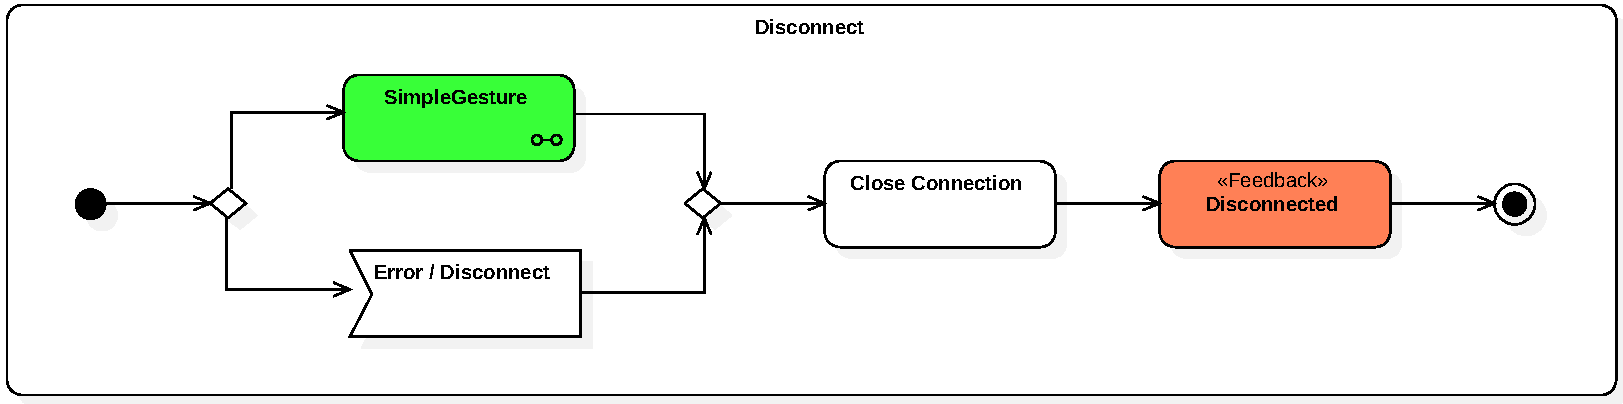
\includegraphics[width=1\textwidth]{bilder/disconnect.pdf}
\caption{Trennen der Verbindung in der Aktivität \textit{Disconnect}.}
\label{fig:disconnect}
\end{figure}

Angestoßen wird der Verbindungsabbau je Gerät entweder durch eine einfache Geste oder durch ein Systemevent, das über einen Verlust der Verbindung informiert (\zb beim Verbindungsabbau durch das verbundene Gerät oder einen Verbindungsfehler). Anschließend wird die Verbindung geschlossen und der Benutzer darüber informiert (\textit{Feedback Disconnect}). Eine synchrone Geste ist an dieser Stelle nicht sinnvoll, da das Schließen der Verbindung sonst nicht von einem Nutzer alleine durchgeführt werden könnte. Würde der Nutzer der Gegenseite seinen Teil der synchronen Geste nicht erfüllen, könnte er das Trennen der Verbindung verhindern.

In der Literatur finden sich einige Hinweise für die (gestenbasierte) Gestaltung der \textit{Disconnect}"=Aktivität, wobei das Spektrum der verwendeten Gesten deutlich eingeschränkter als bei der \textit{Connect}-Aktivität ist.

Um zwei Geräte zu trennen, die per Bump verbunden wurden, schlägt Hinckley ein Auseinanderbewegen der Tablets vor \citep{Hinckley2003}. Sobald ein Tablet erkennt, dass es von dem verbundenen Tablet wegbewegt wird, informiert es dieses über den Verbindungsabbau und gibt ein visuelles (in Form eines zerbrochenen Pfeils, entsprechend dem visuellen Feedback beim \textit{Connect}, siehe Kapitel \ref{subsec:connect}) sowie akustisches Feedback in Form eines "`breaking sounds"'. Beim Erhalt der Nachricht zum Disconnect wiederholt das zweite Tablet beide Feedbacks und baut ebenfalls die Verbindung ab.

Für die Stitch-Geste schlagen Hinckley und Kollegen vor, den Verbindungsabbau einfach über die Auswahl eines Menüpunktes in der Nutzeroberfläche vorzunehmen und verzichten gänzlich auf den Einsatz einer umfangreichen Geste \citep{Hinckley2004}. Hier würde entsprechend dem Modell in Abbildung \ref{fig:disconnect} einfach auf ein Systemevent reagiert, das zweite Gerät würde durch einen Fehler bzw. Timeout über den Verbindungsabbau informiert.

In \citep{Dachselt2009} wird kein Mechanismus zum Verbindungsabbau explizit vorgeschlagen. Allerdings wird die Verbindung per Bluetooth oder Wi-Fi beim Betreten des Raumes aufgebaut, was nahelegt, dass das Verlassen des Raumes entweder als Geste zum Verbindungsabbau interpretiert werden kann oder ein Verlust des Funksignals implizit die Verbindung trennt. Beides ist durch das Modell in Abbildung \ref{fig:disconnect} abbildbar.

Lucero und Kollegen schlagen vor, ein Smartphone durch Aufnehmen von einem Tisch von verbundenen Geräten zu trennen oder das Teilen von Fotos durch Kippen des Smartphones (Tilt-Geste) zu beenden \citep{Lucero2011}. Im ersten Fall wird ein visuelles Feedback angezeigt, für den zweiten Fall schlagen sie ein langes Vibrieren vor. Nimmt der Nutzer sein Gerät vom Tisch, auf dem eine Multiscreen-Interaktion stattgefunden hat, würde man hier eine auf Distanz basierende Geste definieren. Zwar sind die Geräte noch in Sendereichweite, allerdings kann \zb per NFC oder BLE erkannt werden, wann der Abstand einen Schwellwert erreicht, ab dem der Verbindungsabbau ausgelöst wird. Die Tilt-Geste kann ebenfalls als einfache Geste definiert und hier als Auslöser für den Verbindungsabbau eingesetzt werden.

Zusammenfassend lässt sich sagen, dass zwar teilweise einfache Gesten zum Einsatz kommen, um die \textit{Disconnect}-Aktivität zu starten, in vielen Fällen allerdings ein Verlassen des Sendebereiches implizit für das Trennen der Verbindung sorgt. Soll eine festgelegte Distanz zwischen Geräten den Verbindungsabbau auslösen, muss das entsprechend dem "`Leave To Disconnect"' Pattern aus der SysPlace"=Patternsammlung (siehe Anhang \ref{a:patterns_all}) explizit modelliert werden, um \zb mittels \textit{Constraints} auf entsprechende Distanzen reagieren zu können.

\subsection{Statische Sicht -- Domänenmodell}
\label{subsec:domain_model}
Abschließend wird in diesem Kapitel eine statische Sicht des Modells vorgestellt. Während in den vorigen Kapiteln die dynamischen Aspekte von Multiscreen"=Anwendungen durch das Modell erfasst wurden, wird nun als Ergänzung ein Domänenmodell vorgestellt, das die in den Ablaufdiagrammen verwendeten Komponenten erfasst und in Beziehung zueinander setzt.

Abbildung \ref{fig:dm_gestures} zeigt die statische Modellierung von Gesten und den zur Erkennung von Gesten notwendigen Komponenten. Gesten tauchen in jeder Aktivität des Rahmenmodells auf, zum Verbinden / Trennen von Geräten, Auswählen von Dateien oder zum Starten von Dateitransfers. Kapitel \ref{subsec:simple_gesture} und Kapitel \ref{subsec:synchronous_gesture} beschreiben die Gestenerkennung im Detail und führen Begriffe wie \textit{GestureEvent} und \textit{Con\-straint} ein, die in der statischen Sicht wiederzufinden sind. Im Zentrum steht dabei jeweils der allgemeine Begriff der Geste, der weiter in einfache (\textit{SimpleGesture}) und synchrone (\textit{SynchronousGesture}) Gesten unterteilt wird, für die es jeweils konkrete Ausprägungen analog zum SysPlace-Patternkatalog bzw. der analysierten Literatur gibt.  Es besteht zudem eine Abhängigkeit zwischen \textit{SynchronousGesture} und \textit{SimpleGesture}. Da die Erkennung einer synchronen Geste immer die Erkennung von zwei einfachen Gesten voraussetzt, wird diese als Komposition einfacher Gesten abgebildet.

Im rechten Teil des Diagramms finden sich zudem die Konzepte von \textit{Constraints} und \textit{GestureEvents} wieder. Wird eine Geste erkannt, wird ein sog. \textit{GestureEvent} erstellt, das spezifische Parameter über die Geste bereitstellt (wie \zb Anfangs- und Endkoordinaten einer Swipe-Geste). Diese Parameter können mit vordefinierten \textit{Constraints} verglichen werden, um eine Geste mit Qualitätskriterien auszustatten, die zum jeweiligen Anwendungsfall passen.

Zudem sind zur Erkennung einer konkreten Geste immer bestimmte Geräteeigenschaften wie vorhandene Sensoren notwendig, die hier als \textit{Capabilities} erfasst wurden und den \textit{required}-Annotationen der Gerstenerkennung entsprechen (s. Modell in Abbildung \ref{fig:swipe_recognition}). Dadurch lassen sich durch das statische Modell Abhängigkeiten zwischen verwendeten Erkennungsalgorithmen und benötigter Hard- oder Software herstellen, wodurch eine der Kernanforderungen an das Modell erfüllt wird.
\begin{sidewaysfigure}
\centering
\includegraphics[page=2,width=\textwidth,height=0.58\textheight]{bilder/domain_model.pdf}
\caption{Domänenmodell für die Gestenerkennung.}
\label{fig:dm_gestures}
\end{sidewaysfigure}

Das Spektrum möglicher \textit{Capabilities} wird in Abbildung \ref{fig:dm_capabilities} modelliert. Der allgemeine Begriff der \textit{Capability} aus Abbildung \ref{fig:dm_gestures} wird hier in Kategorien unterteilt:
\begin{itemize}
\item \textit{Input}: Erfassen von direkten oder indirekten Nutzereingaben.
\item \textit{Output}: Ausgabe von Systemreaktionen.
\item \textit{Proximity}: Wahrnehmen von Geräten in der Umgebung.
\item \textit{Connectivity}: Herstellen von Netzwerkverbindungen.
\end{itemize}

Als \textit{Input} gelten dabei alle Geräteeigenschaften, die in irgendeiner Form Eingaben des Nutzers verarbeiten. Während Tastatur oder Maus direkte Nutzereingaben ermöglichen, erfassen \zb Beschleunigungssensoren auch Eingaben, die der Nutzer eventuell unbewusst tätigt. Die \textit{Capabilities} des Modells zur Gestenerkennung in Abbildung \ref{fig:dm_gestures} sind zumeist vom Typ \textit{Input}, oft in Form eines Touchscreens (\zb zur Swipe-Erkennung) oder eines Bewegungs- und Lagesensors.

Unter \textit{Output} werden alle Geräteeigenschaften zusammengefasst, die Ausgaben des Systems ermöglichen (s. auch Kapitel \ref{subsec:connectivity}), wie \zb Bildschirm, Vibration oder Sound. Diese sind vor allem für die Definition der \textit{Feedback}-Aktivitäten innerhalb der Ablaufbeschreibungen relevant.

Eigenschaften vom Typ \textit{Connectivity} spezifizieren den \textit{Channel}, der in den Aktivitäten \textit{Connect}, \textit{Transfer} und \textit{Disconnect} des Rahmenmodells eine wichtige Rolle für Multiscreen-Interaktionen spielt. Die Art des \textit{Channels} legt fest, welche Infrastruktur für die Realisierung von Multiscreen-Anwendungen benötigt wird. Entsprechend Kapitel \ref{subsec:connectivity} wird zwischen Ad-Hoc- und Infrastruktur"=Netzwerkfähigkeit unterschieden.

Die Menge aller Geräteeigenschaften, die von einer Multiscreen-Anwendung benötigt werden, ergeben als Komposition ein \textit{Device}, das die notwendige Hard- und Software für die Anwendung bereitstellt. Ein Gerät kann demzufolge allgemein als eine Menge benötigter Eigenschaften modelliert werden.

\begin{sidewaysfigure}
\centering
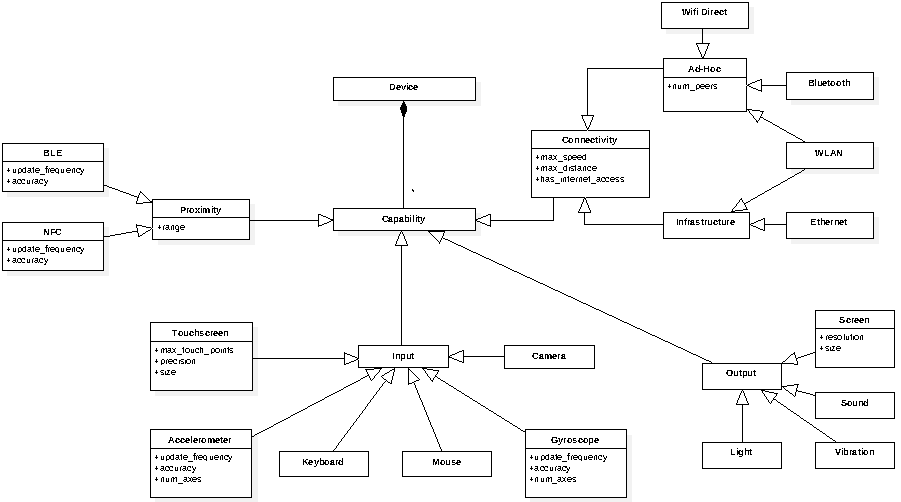
\includegraphics[page=1, width=\textwidth, height=0.58\textheight]{bilder/domain_model.pdf}
\caption{Domänenmodell der Geräteeigenschaften (\textit{Capabilities}).}
\label{fig:dm_capabilities}
\end{sidewaysfigure}

Abbildung \ref{fig:dm_input_output} zeigt den Zusammenhang zwischen \textit{User Interactions}, \textit{Feedback} und \textit{Capabilities}. Die verschiedenen farblich markierten \textit{User Interaction}- und \textit{Feedback}"=Aktivitäten innerhalb der Ablaufmodelle lassen sich so analog zu den Gesten mit benötigten Geräteeigenschaften in Zusammenhang bringen. Da Systemfeedback und Nutzereingaben auch multimodal sein können, wird eine \textit{User Interaction} bzw. ein \textit{Feedback} hier als Komposition einzelner Elemente beschrieben, die jeweils eine \textit{Capability} des Gerätes voraussetzen. Die Gesamtheit aller \textit{User Interactions} und \textit{Feedbacks} in einer Multiscreen-Anwendung hat somit wiederum einen Einfluss auf das \textit{Device} in Abbildung \ref{fig:dm_capabilities}.
 
\begin{figure}[h]
\centering
\includegraphics[page=3, width=\textwidth]{bilder/domain_model.pdf}
\caption{Aufbau von \textit{User Interactions} und \textit{Feedback} mit Bezug zu \textit{Capabilities}.}
\label{fig:dm_input_output}
\end{figure}

Der letzte Aspekt, der durch das statische Modell der Vollständigkeit halber noch erfasst werden muss, ist die \textit{Selection}, die in den Aktivitäten \textit{Select} und \textit{Transfer} des Rahmenmodells eine Rolle spielt und nach Kapitel \ref{sec:select} die Ausprägungen \textit{Command}, \textit{File}, \textit{MultipleFiles} oder \textit{Stream} haben kann, wobei \textit{MultipleFiles} eine Aggregation vom Typ \textit{File} ist und hier nicht separat aufgeführt wird. Abbildung \ref{fig:dm_selection} zeigt das entsprechende Domänenmodell dazu.

\begin{figure}[h]
\centering
\includegraphics[page=4, width=0.7\textwidth]{bilder/domain_model.pdf}
\caption{Domänenmodell für die \textit{Selection}.}
\label{fig:dm_selection}
\end{figure}

Diese statischen Sichten sind eine wichtige Ergänzung des Modells, da sie es um einige Möglichkeiten erweitern. Sie verdeutlichen die Wiederverwendbarkeit von Komponenten, die nur einmal modelliert werden müssen, um sie in die verschiedenen dynamischen Sichten einfügen zu können. Zudem sind sie ein Ansatzpunkt zur Erweiterung des Modells, indem \zb neue Technologien zur Ein- und Ausgabe oder neue Gesten in die statische Struktur aufgenommen und in den dynamischen Modellen verwendet werden können. 

Es ist außerdem möglich, aus einem dynamischen Modell das zugehörige statische Modell abzuleiten oder umgekehrt. So kann eine Multiscreen-Anwendung beliebig dynamisch modelliert und anschließend jede Komponente statisch erfasst werden, um Rückschlüsse über Mindestanforderungen an Geräte zu ziehen oder benötigte Parameter zusammenzufassen. Umgekehrt ist es möglich, das statische Modell als Basis vorab zu definieren und die dynamischen Aspekte daraus abzuleiten. Es ist \zb denkbar, dass nur ein bestimmter Satz an Geräteeigenschaften zur Verfügung steht und die Design-Möglichkeiten der dynamischen Aspekte einer Multiscreen-Anwendung einschränkt.

\chapter{Validierung des Modells}
\label{ch:validierung}

In diesem Kapitel wird eine Bewertung des erarbeiteten Modells aus Kapitel \ref{ch:modell} vorgenommen. Dazu wird zunächst eine qualitative Aussage getroffen, zu welchem Grad die Anforderungen, die in Kapitel \ref{sec:requirements} formuliert wurden, durch das Modell erfüllt werden. Anschließend werden zwei Gruppen von Patterns aus dem SysPlace-Patternkatalog, basierend auf der Bump- bzw. Approach-Geste, exemplarisch durch das Modell beschrieben. Die Flexibilität des Modells soll dadurch verdeutlicht werden, dass beide Gruppen unterschiedliche Technologien voraussetzen und unterschiedliche Einsatzgebiete haben und dennoch einheitlich erfasst werden können. Darauf aufbauend wird diskutiert, inwiefern sich von diesen Beispielen auf die Anwendungsmöglichkeiten für die übrigen Patterns des SysPlace-Patternkataloges schließen lässt.

\section{Qualitative Bewertung der Anforderungserfüllung}
Die Anforderungen an das Modell aus Kapitel \ref{sec:requirements} lassen sich in drei Gruppen zusammenfassen. Es gibt Anforderungen an
\begin{itemize}
\item die Erfassung der Gestenerkennung,
\item die Beschreibung der anschließenden Systemreaktion und
\item die Verwendbarkeit des Modells.
\end{itemize}
In diesem Kapitel wird gezeigt, welche Aspekte des Modells zur Erfüllung einzelner Anforderungen dieser Gruppen beitragen. 

Für die Gestenerkennung werden in den Anforderungen einige Aspekte definiert, die durch das Modell abbildbar sein sollen:
\begin{itemize}
\item Direkte oder indirekte Eingaben des Nutzers,
\item abstrakte Beschreibung des Algorithmus und mögliche Alternativen,
\item Einschränkungen der Gestenerkennung,
\item Hard- und Softwarevoraussetzungen für die Gestenerkennung,
\item Kommunikationsprotokolle für synchrone Gesten und
\item Wiederverwendbarkeit von Teilkomponenten.
\end{itemize}
In Kapitel \ref{subsec:simple_gesture} wird das Modell für die Beschreibung einfacher Gesten vorgestellt, welches aus zwei Teilen besteht (siehe Abbildung \ref{fig:gesture_detection}):
\begin{enumerate}
\item \textit{Recognize Gesture}: Eine Geste aufgrund von Sensordaten erkennen.
\item \textit{Check Constraints}: Einschränkungen der erkannten Geste prüfen.
\end{enumerate} 
Die Aktivität \textit{Recognize Gesture} beschreibt abstrakt den Erkennungsalgorithmus für eine Geste (siehe Abbildung \ref{fig:swipe_recognition} für eine exemplarische Anwendung) mittels eines Zustandsdiagramms. Hard- und Software"=Voraussetzungen werden in Form von Parametern und benötigten Sensoren als Annotationen beschrieben. Die Eingaben des Nutzers werden als System-Events dargestellt, die Transitionen zwischen den Zuständen auslösen. Berechnungen, die bei diesen Transitionen ausgeführt werden, können über Pseudo-Code-Annotationen abstrakt beschrieben werden. 

Das Ergebnis einer Gestenerkennung ist ein \textit{GestureEvent}, das Informationen über die erkannte Geste beinhaltet, die im nächsten Schritt (\textit{Check Constraints}) geprüft werden können. Dadurch wird die Anforderung an die Einschränkung erkannter Gesten erfüllt, zudem wird durch die Trennung zwischen Erkennung und Einschränkung eine Wiederverwendbarkeit der einzelnen Teile erreicht. Der Erkennungsalgorithmus kann beliebig ausgetauscht werden, sofern das gleiche \textit{GestureEvent} an die Aktivität \textit{Check Constraints} übergeben wird.

Entsprechend den Anforderungen wird in Kapitel \ref{subsec:synchronous_gesture} ein Kommunikationsprotokoll beschrieben, das der einfachen Gestenerkennung noch einen Vergleich zweier \textit{GestureEvents} hinzufügt (\textit{Gesture Event Matching}) und dadurch die Erkennung synchroner Gesten ermöglicht. Es wurde ein genereller Ablauf für alle synchronen Gesten erarbeitet, der eine hohe Austauschbarkeit der einfachen Gestenerkennung und der Vergleichsaktivität ermöglicht. Sofern die zwei \textit{GestureEvents}, also die Outputs der einfachen Gestenerkennungen, gleich den zwei Inputs des Vergleichsschritts sind, kann eine beliebige Kombination einfacher zu synchronen Gesten vorgenommen werden, wodurch wiederum eine hohe Wiederverwendbarkeit von Teilkomponenten für die synchrone Gestenerkennung gegeben ist.

Hinsichtlich der verschiedenen Systemreaktionen, die auf das Erkennen einer einfachen oder synchronen Geste folgen, wurden in den Anforderungen folgende Aspekte genannt, die durch das Modell darstellbar sein müssen:
\begin{itemize}
\item Vollständige Ablaufbeschreibung,
\item Vor- und Nachbedingungen bzw. Objektfluss,
\item Interaktionsmöglichkeiten des Nutzers,
\item Rückmeldungen (Feedback) des Systems,
\item Implikation der gewählten Geste auf den Ablauf und
\item Alternativen und Fehlerfälle.
\end{itemize}

In Kapitel \ref{subsec:model_overview} wurde zunächst ein Überblick über den Lebenszyklus einer Mul\-ti\-screen"=Anwendung gegeben, die Kapitel zu den Aktivitäten \textit{Connect} (\ref{subsec:connect}), \textit{Select} (\ref{sec:select}), \textit{Tranfer} (\ref{subsec:transfer}) und \textit{Disconnect} (\ref{subsec:disconnect}) vertiefen diese Sicht jeweils um detaillierte Beschreibungen in Form von Ablaufdiagrammen. Jede dieser Aktivitäten kann mit Vorbedingungen (\zb erforderlicher Auslöser oder benötigter Input) und Nachbedingungen (\zb ausgewählte Daten oder geöffnete Verbindungen) versehen werden. Platzhalter innerhalb der Ablaufbeschreibungen beschreiben die Stellen, an denen der Nutzer mit dem System interagieren kann (\textit{User Interaction}), bzw. an der das System dem Nutzer eine Rückmeldung (\textit{Feedback}) geben kann. Sofern die Wahl zwischen einfacher oder synchroner Geste eine Implikation auf den Ablauf hat, wurden beide Alternativen modelliert. Mögliche Fehlerfälle wurden in Form von System-Events erfasst, deren Behandlung ebenfalls Teil der Ablaufbeschreibung ist und Feedback beinhalten kann.
 
An die Verwendbarkeit des Modells gibt es zusammengefasst folgende Anforderungen:
\begin{itemize}
\item Wahl einer verständlichen Repräsentation für Entwickler und Interaktionsdesigner,
\item Verfügbarkeit von Tools zur Arbeit mit dem Modell,
\item Aussagefähigkeit über Mindestanforderungen an Hard- und Software,
\item einfache Erweiterbarkeit und
\item Einsatz als Kommunikationsmittel.
\end{itemize}
Durch die Wahl der \acs{UML} als Modellierungssprache werden die ersten beiden Anforderungen adressiert, wie schon in der Einleitung zu Kapitel \ref{ch:modell} dargelegt wurde. 

Um eine Aussage über die Mindestanforderungen an Hard- und Software treffen zu können, wurden die dynamischen Modelle in Kapitel \ref{subsec:domain_model} um eine statische Sicht, das Domänenmodell, erweitert. Indem man alle verwendeten Entitäten der erstellten Ablaufbeschreibungen in einer statischen Sicht aggregiert, kann abstrakt die benötigte Umgebung für den Einsatz des beschriebenen Patterns abgeleitet werden. Umgekehrt ist es auch möglich, die verfügbare Infrastruktur zunächst im Domänenmodell zu erfassen, um die Gestaltungsmöglichkeiten der dynamischen Modelle auf diesen Ausschnitt zu beschränken.

Auch die Erweiterbarkeit des Modells wird über die statische Sicht realisiert. Werden \zb eine neue Übertragungstechnologie oder ein weiteres Ausgabegerät verfügbar, können diese in das Domänenmodell aufgenommen und an den entsprechenden Stellen im dynamischen Modell eingesetzt werden. So können \zb neue Sensoren alternative Möglichkeiten zur Gestenerkennung eröffnen, die wiederum dynamisch erfasst und als Alternative zur bisherigen Gestenerkennung dokumentiert werden können.

Erstellte Modelle können als Dokumentation und somit als Kommunikationsmittel für die Gestaltung von Multiscreen-Interaktionen verwendet werden. Indem die wichtigen Gestaltungsentscheidungen wie Erkennungsalgorithmen oder Feedbacks als austauschbare Elemente in einen übergeordneten Ablauf eingesetzt werden, können mittels des Modells Fragestellungen wie die folgenden diskutiert werden:
\begin{itemize}
\item Wie wäre es, wenn wir als Erfolgs-Feedback an \textit{dieser Stelle} noch zusätzlich den Sound abspielen, den wir auch \textit{hier} verwenden?
\item Können wir \textit{diese Geste} auch einsetzen, wenn kein Beschleunigungssensor verfügbar ist?
\item Würde die Übertragung beschleunigt, wenn wir \textit{den Übertragungskanal} von Bluetooth auf Wi-Fi Direct umstellen?
\item An welchen Stellen wird in der Anwendung \textit{diese Dialogbox} angezeigt?
\end{itemize}
Neben den visuellen Aspekten der Diagramme sind dabei auch die eingeführten Begrifflichkeiten des Domänenmodells hilfreich. Die Verwendung bzw. individuelle Anpassung der verwendeten Begrifflichkeiten fördert eine einheitlich genutzte und verstandene Sprache im Projektteam. Um die technische Realisierung erstellter Modellinstanzen zu unterstützen, wird in Kapitel \ref{sec:framework} ein Ansatz zur Entwicklung eines Frameworks vorgestellt, das die Übersetzung modellierter Konzepte in ausführbaren Code erleichtern könnte.

\section{Exemplarische Instanziierungen des Modells}
\subsection{Bump-Patterns}
\label{subsec:bump_validation}
In diesem Kapitel wird das Modell zur technischen Beschreibung aller Patterns angewendet, die auf einer Bump-Geste basieren (siehe Anhang \ref{a:patterns_all}):
\begin{itemize}
\item Bump To Connect
\item Bump To Give
\item Bump To Take
\item Bump To Exchange
\end{itemize}
Die Ausgestaltung der Details ist dabei stark angelehnt an die Ideen in \citep{Hinckley2003}, wobei auch Variationen der Details denkbar sind. Es wird lediglich versucht, eine exemplarische, konsistente Beschreibung einer Gruppe von Patterns zu erstellen.

Grundlegend für alle vier Patterns ist die Beschreibung der verwendeten Bump-Geste. Dem Modell in Abbildung \ref{fig:gesture_detection} entsprechend muss dazu zunächst die Erkennung der Geste auf einem Gerät beschrieben werden. Abbildung \ref{fig:bump_recognize} zeigt eine detaillierte Beschreibung der Bump-Geste mittels des Modells.
\begin{figure}[h]
\centering
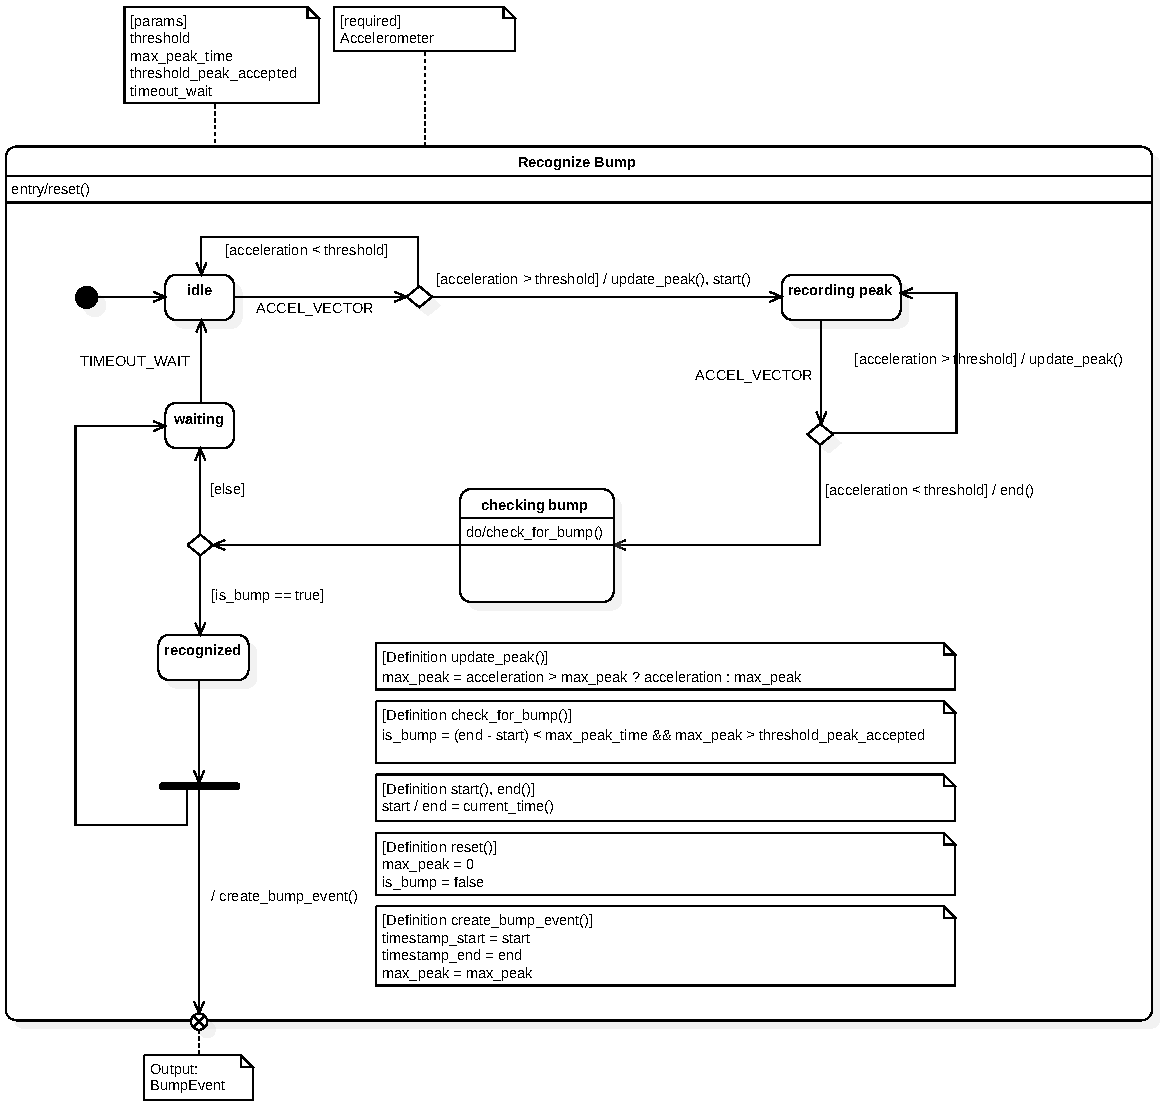
\includegraphics[width=1\textwidth]{bilder/bump/recognize}
\caption{Erkennung einer Bump-Geste entsprechend der \textit{Gesture Detection} in Abbildung \ref{fig:gesture_detection}.}
\label{fig:bump_recognize}
\end{figure}

Der Algorithmus basiert auf der Erkennung eines sog. \textit{Peaks} (deut. Spitze) in den Beschleunigungswerten. Vorausgesetzt werden dafür ein Beschleunigungssensor und vier Parameter:
\begin{itemize}
\item \textit{threshold}: Schwellwert, ab dem vom Auftreten eines Peaks ausgegangen wird.
\item \textit{max\_peak\_time}: Maximale Zeit zwischen Übertretungen des Schwellwerts, also die "`Breite"' des Peaks.
\item \textit{threshold\_peak\_accepted}: Schwellwert, ab dem ein Peak akzeptiert wird (Beschleunigungswert, der innerhalb des Peaks mindestens überschritten werden muss).
\item \textit{timeout\_wait}: Wartezeit nach Bump-Erkennung.
\end{itemize}

Im Anfangszustand werden so lange Beschleunigungsvektoren gelesen, bis der \textit{thresh\-old}-Wert überschritten wurde. Anschließend wird bis zum nächsten Überschreiten der Schwelle gewartet, also dem Ende des Peaks. Dazwischen wird die Maximalbeschleunigung überschrieben (in \textit{update\_peak()}), wenn ein höherer Wert als der bisher maximale gelesen wurde. Nach erneutem Unterschreiten der Schwelle wird geprüft, ob die Spitze das zeitliche Fenster \textit{max\_peak\_time} nicht über- und den erforderlichen Schwellwert für die Beschleunigung nicht unterschritten hat. Sind diese Bedingungen erfüllt, wird die Bump-Geste erkannt und das entsprechende \textit{BumpEvent} generiert, ansonsten beginnt die Erkennung von vorne. 

In beiden Fällen wird eine Wartezeit von \textit{timeout\_wait} abgewartet, bevor die Erkennung erneut beginnt, um zu schnelle Folgen von Bump-Erkennungen auszuschließen. Für die Bump-Erkennung wurden keine Constraints verwendet, dies wäre allerdings \zb für die minimal zulässige Beschleunigung denkbar, je nachdem, ob dieser Wert individuell einstellbar oder fest sein soll.

\begin{figure}[h]
\centering
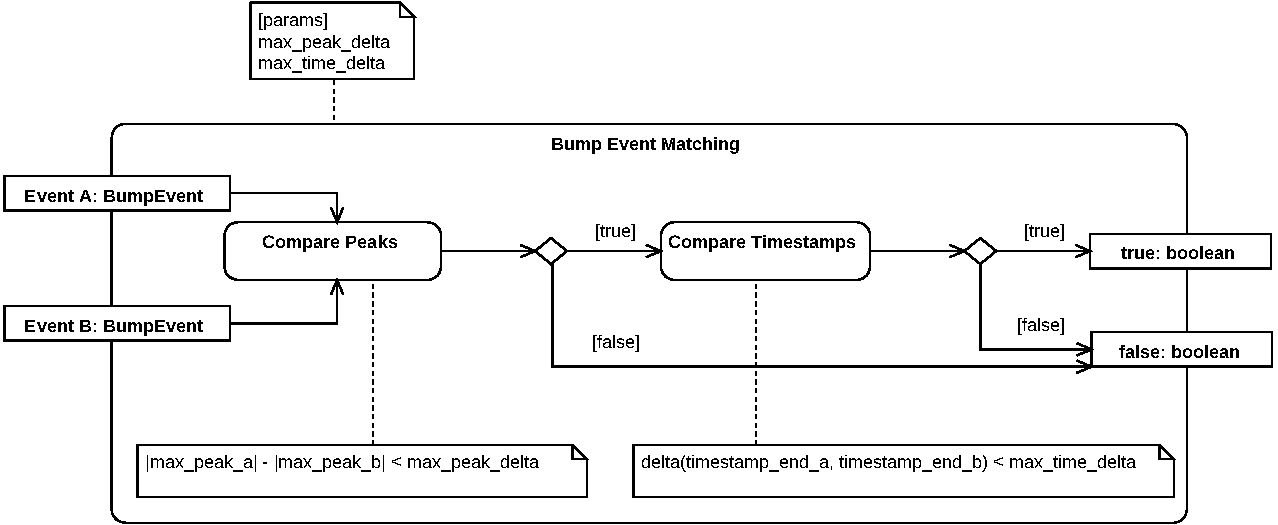
\includegraphics[page=1,width=1\textwidth]{bilder/bump/event_matching}
\caption{Erkennung einer synchronen Bump-Geste entsprechend dem Modell in Abbildung \ref{fig:sync_gesture_detection}.}
\label{fig:bump_event_matching}
\end{figure}

Da es sich beim Bump um eine synchrone Geste handelt, muss noch der Vergleich zweier Bump-Events entsprechend dem Modell in Abbildung \ref{fig:sync_gesture_detection} beschrieben werden. Abbildung \ref{fig:bump_event_matching} zeigt den Vergleich von zwei Bump-Events anhand der maximalen Beschleunigung an der Spitze (mit einer erlaubten Differenz von \textit{max\_peak\_delta}) und dem zeitlichen Abstand beider Bump-Events (mit einer maximalen Differenz von \textit{max\_time\_delta}). Sind beide Bedingungen erfüllt, wird die synchrone Geste erkannt und beide Geräte über ihren Kommunikationspartner informiert.

Solch eine Erkennung ist auch in den alternativen Ausprägungen des Modells in Anhang \ref{a:sync_gestures} möglich, je nachdem welche Infrastruktur gegeben ist. In \citep{Hinckley2003} wird vorgeschlagen, alle Geräte über eine WLAN-Infrastruktur miteinander zu vernetzen und ein Gerät als Server für die Gesten-Erkennung zu verwenden. Diese Variante wird auch in diesem Beispiel vorausgesetzt.

Aufbauend auf der Erkennung der Bump-Geste können jetzt die Patterns der einzelnen Kategorien näher spezifiziert werden. Abbildung \ref{fig:bump_connect} beschreibt das Pattern "`Bump To Connect"' und zeigt den Ablauf des Verbindungsaufbaus zwischen zwei Geräten, nachdem eine Bump-Geste erkannt wurde. Das Gerät, welches sich im Netzwerk auffindbar macht, spielt ein kurzes Geräusch ab. Anschließend wird das Verbindungsprotokoll ausgehandelt. 

\begin{sidewaysfigure}
\centering
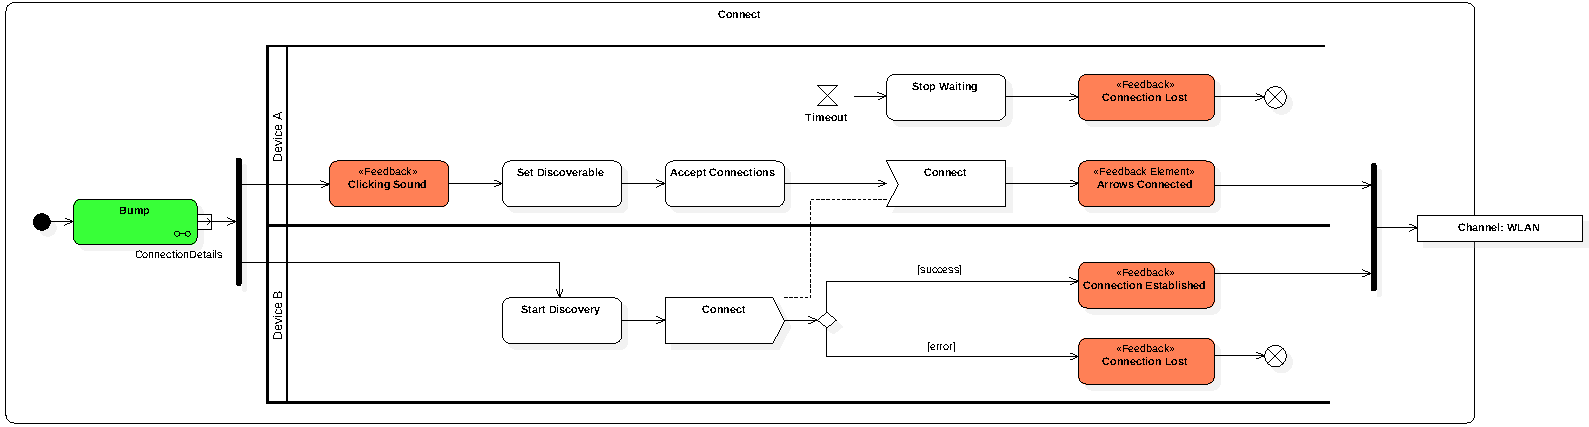
\includegraphics[width=1\textwidth]{bilder/bump/connect}
\caption{Ablauf des Patterns Bump-To-Connect -- Verbinden zweier Geräte mittels Bump-Geste.}
\label{fig:bump_connect}
\end{sidewaysfigure}

Bei Erfolg wird ein zusammengesetztes Feedback aus visuellen und akustischen Hinweisen auf beiden Geräten ausgegeben. Im Nichterfolgsfall gibt es ein negatives Feedback. In Abbildung \ref{fig:bump_dm_feedback} findet sich eine statische Beschreibung der verwendeten individuellen Feedbacks und der benötigten \textit{Capabilities}, ansonsten unterliegt die \textit{Connect}-Aktivität einem starren Ablauf, der auch für andere Gesten gleich ablaufen würde. Das Ergebnis der Aktivität ist ein \textit{Channel} vom Typ WLAN, wie oben definiert wurde.

\begin{figure}[h]
\centering
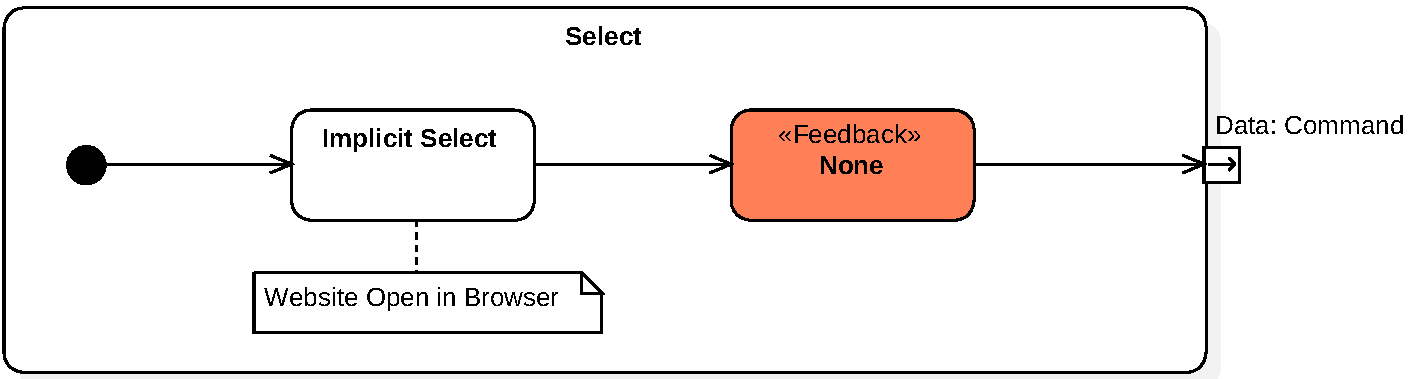
\includegraphics[page=1,width=0.7\textwidth]{bilder/bump/select}
\caption{Implizite Auswahl einer geöffneten Webseite im Browser des Nutzers als \textit{Command}.}
\label{fig:bump_command_select}
\end{figure}

Zwar sieht kein Pattern explizit eine \textit{Select}-Aktivität vor, dennoch ist diese die Grundlage für Patterns mit \textit{Transfer}-Aktivitäten (s. Modell in Abbildung \ref{fig:model_overview} bzw. \ref{fig:model_overview_alternative}). Als einfaches Beispiel soll hier der Anwendungsfall aus \citep{Hinckley2003} angenommen werden, in dem eine geöffnete Webseite mit einem anderen Benutzer per Bump-Geste geteilt werden soll. Hier ist die \textit{Selection} vom Typ \textit{Command} (vgl. Kapitel \ref{sec:select}), eine Beschreibung des Ablaufes zeigt Abbildung \ref{fig:bump_command_select}. Es ist auch möglich, dass ein Nutzer gar nichts auswählt und nur eine leere Anwendung geöffnet hat. Dieser Fall ist in Abbildung \ref{fig:bump_empty_select} beschrieben. Mit diesen beiden Definitionen für mögliche \textit{Select}-Aktivitäten lassen sich die drei übrigen Bump-Patterns beschreiben.

\begin{figure}[h]
\centering
\includegraphics[page=2,width=0.7\textwidth]{bilder/bump/select}
\caption{Keine Auswahl durch den Benutzer.}
\label{fig:bump_empty_select}
\end{figure}

Abbildung \ref{fig:bump_transfer} zeigt das Anstoßen eines Datentransfers mittels Bump-Geste. Vorbedingungen sind eine bestehende WLAN-Verbindung und ein ausgewählter \textit{Command}. Wird nun eine synchrone Bump-Geste erkannt, wird der Transfer gestartet. Die Details der Übertragung sind in Abbildung \ref{fig:bump_transfer_selection} dargestellt. Hier wurden einige Schritte, die im Gesamtmodell in Abbildung \ref{fig:transfer_selection} vorgesehen sind, weggelassen. Es wird davon ausgegangen, dass die Übertragung eines \textit{Commands} unmittelbar stattfindet und kein Feedback über den Fortschritt benötigt wird. Zudem gibt zunächst nur das sendende Gerät ein Feedback in Form eines "`Teleport"'-Sounds aus, um zu signalisieren, dass es den Befehl versendet hat. Auf dem Empfangsgerät ist kein zusätzliches Feedback notwendig, da bereits das Öffnen der Webseite im Browser (die Ausführung des \textit{Command}) ein Feedback an den Nutzer darstellt. 
 
\begin{figure}[h]
\centering
\includegraphics[page=2,width=0.7\textwidth]{bilder/bump/transfer}
\caption{Start des Transfers mittels Bump-Geste.}
\label{fig:bump_transfer}
\end{figure}

Mittels dieser Beschreibung lassen sich die Patterns "`Bump To Give"', "`Bump To Take"' und "`Bump To Exchange"' beschreiben. Sollte auf einem Gerät eine leere \textit{Selection} vorhanden sein (siehe Abbildung \ref{fig:bump_empty_select}), so wird höchstens ein "`Bump To Take"' durchgeführt, wenn auf dem anderen Gerät der entsprechende \textit{Command} ausgewählt wurde. Das sendende Gerät realisiert dann automatisch ein "`Bump To Give"'. Ist auf beiden Geräten eine Webseite geöffnet, also auf beiden Geräten eine Selektion vorhanden (siehe Abbildung \ref{fig:bump_command_select}), wird ein Austausch von Webseiten durchgeführt, also ein "`Bump To Exchange"'. Durch eine Definition von Constraints könnte eine genauere Rollenverteilung der "`Give"'-, "`Take"'- und "`Exchange"'-Geräte erreicht werden.

\begin{figure}[h]
\centering
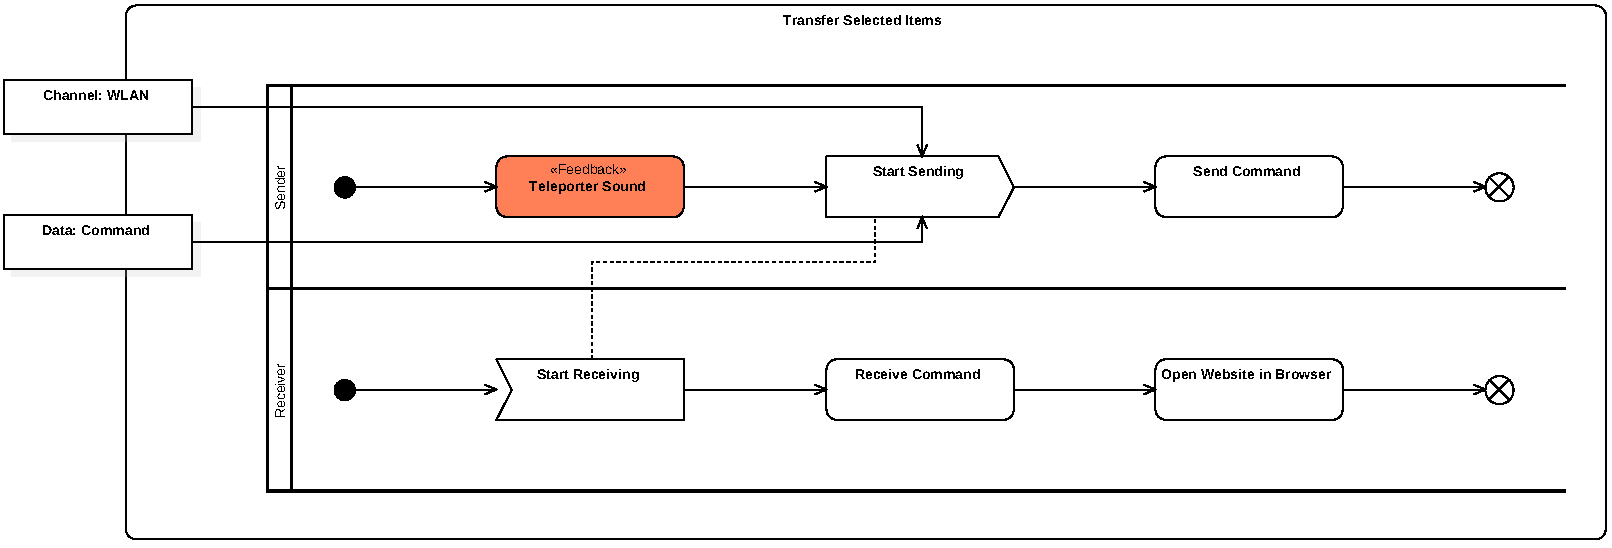
\includegraphics[page=1,width=\textwidth]{bilder/bump/transfer}
\caption{Übertragen des \textit{Commands} und Öffnen der Webseite auf dem Empfangsgerät.}
\label{fig:bump_transfer_selection}
\end{figure}

\begin{figure}[h]
\centering
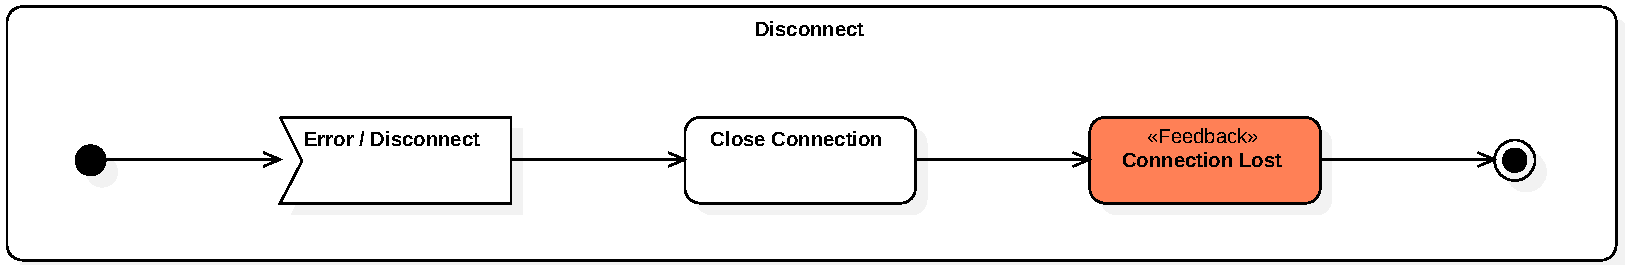
\includegraphics[width=1\textwidth]{bilder/bump/disconnect}
\caption{Trennen der Verbindung zwischen den Geräten.}
\label{fig:bump_disconnect}
\end{figure}

Der Vollständigkeit halber muss nach dem Lebenszyklusmodell (siehe Abbildung \ref{fig:model_overview} bzw. \ref{fig:model_overview_alternative}) noch das Trennen der Verbindung definiert werden (siehe Abbildung \ref{fig:bump_disconnect}). Dazu wird keine Bump-Geste verwendet, da ein "`Bump To Disconnect"'-Pattern im Pattern-Katalog nicht vorgesehen ist und auch nicht sinnvoll wäre. Somit wird hier einfach davon ausgegangen, dass durch Verlassen des Funkbereiches oder ein eventuelles Timeout-Event irgendwann ein Trennen der Verbindung erfolgt, über das der Nutzer durch ein Feedback informiert wird. 

\begin{figure}[h]
\centering
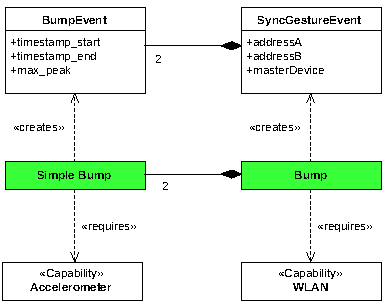
\includegraphics[page=1,width=0.5\textwidth]{bilder/bump/domain_model}
\caption{Statische Sicht der Erkennung von Bump-Gesten und den dazu benötigten \textit{Capabilities}.}
\label{fig:bump_dm_gesture}
\end{figure}

Aus der Gestenbeschreibung in Abbildungen \ref{fig:bump_recognize} und \ref{fig:bump_event_matching} ergibt sich das statische Modell in Abbildung \ref{fig:bump_dm_gesture}, das die benötigten \textit{Capabilities} berücksichtigt und die erzeugten Events beschreibt. Die verwendeten Feedbacks der verschiedenen Ablaufbeschreibungen wurden in Abbildung \ref{fig:bump_dm_feedback} gesammelt und ebenfalls mit den benötigten \textit{Capabilities} versehen.

\begin{figure}[h!]
\centering
\includegraphics[page=2,width=1\textwidth]{bilder/bump/domain_model}
\caption{Von Bump-Patterns verwendete einfache und zusammengesetzte Feedbacks.}
\label{fig:bump_dm_feedback}
\end{figure}

Aus den gesammelten Anforderungen an Geräteeigenschaften kann ein abstraktes Gerät modelliert werden, das mindestens notwendig ist, um die Pattern umzusetzen, wie in Abbildung \ref{fig:bump_dm_device} zu sehen. Jedes Bump-Pattern benötigt für die Erkennung der Bump-Geste somit mindestens einen Beschleunigungssensor und muss WLAN-fähig sein (sowohl zum Synchronisieren von \textit{BumpEvents} als auch zum Transfer von Daten). Für die meisten Feedbacks ist Bild- und Tonausgabe wichtig, da oft kombiniertes Feedback eingesetzt wird.

\begin{figure}[h!]
\centering
\includegraphics[page=3,width=1\textwidth]{bilder/bump/domain_model}
\caption{Statische Sicht aller benötigten \textit{Capabilities} und deren Zusammenfassung in einem abstrakten Gerät.}
\label{fig:bump_dm_device}
\end{figure}

\begin{figure}[h!]
\centering
\includegraphics[page=4,width=0.5\textwidth]{bilder/bump/domain_model}
\caption{Verwendete \textit{Selection}-Typen.}
\label{fig:bump_dm_selection}
\end{figure}
Abbildung \ref{fig:bump_dm_selection} ergänzt das statische Modell um die verwendeten \textit{Selection}-Typen \textit{Command} und \textit{Empty}, je nachdem ob eine Webseite geöffnet ist oder nicht.

Die statischen Sichten sind nicht extra nach Pattern-Kategorie unterteilt, sondern umfassen jeweils die gesamte Gruppe von Bump-Patterns. Möchte man nur die Anforderungen an ein einzelnes Pattern beschreiben, müssen entsprechend \textit{Feedbacks} und \textit{Capabilities} entfernt werden, die in dem Pattern nicht benötigt werden. Das würde allerdings für die Bump-Patterns keinen großen Unterschied machen, da ähnliche \textit{Capabilities} von allen Patterns vorausgesetzt werden.

Würden statt einer geöffneten Webseite Dateien oder ein Datenstrom übertragen, müsste man nicht das gesamte Modell anpassen, sondern nur die Aktivitäten \textit{Transfer} und \textit{Select} und die dort verwendeten Feedbacks. Somit sind Teile des Modells wie die Gestenerkennung wiederverwendbar, auch Teile der Feedbacks wie bspw. abgespielte Sounds können dort wiederverwendet werden. Durch Erweiterung des statischen Modells kann wiederum darauf geschlossen werden, ob dadurch neue \textit{Capabilities} benötigt werden. Ändert sich das statische Modell in der Hinsicht nicht, kann das Pattern auf den bisher unterstützten Geräten weiterhin eingesetzt werden.

\subsection{Approach-Patterns}
\label{subsec:approach_validation}
Analog zu den Bump-Patterns wird in diesem Kapitel die Gruppe der Patterns besprochen, die auf der Approach-Geste, also einem Annähern eines Gerätes an ein anderes, basieren. Der SysPlace-Patternkatalog sieht eine Gruppe von vier Patterns vor, die auf dieser Geste basieren (siehe Anhang \ref{a:patterns_all}):
\begin{itemize}
\item Approach To Connect,
\item Approach To Give,
\item Approach To Take und
\item Approach To Extend.
\end{itemize}
Zudem gibt es das Pattern "`Leave To Disconnect"', das sich durch die gleichen Komponenten erfassen lässt, wie später gezeigt wird.

Wie in Kapitel \ref{ch:grundlagen} beschrieben gibt es verschiedene Technologien, um Geräte in der Umgebung zu erkennen und ggf. den Abstand zu diesen zu messen. Für die Modellierung der Approach-Patterns wird hier die iBeacon-Technologie verwendet, da diese inzwischen weite Verbreitung findet und das zugrunde liegende \acs{BLE} in vielen neueren Geräten vorhanden und einfach einzusetzen ist. Alle Beschreibungen lassen sich aber ebenso mit wenig Aufwand auf andere Protokolle wie \zb Eddystone übertragen.
\begin{figure}[h]
\centering
\includegraphics[page=1,width=0.7\textwidth]{bilder/approach/recognize}
\caption{Monitoring zum einmaligen Erkennen neuer Geräte bei Annäherung.}
\label{fig:approach_monitoring}
\end{figure}

Abbildung \ref{fig:approach_monitoring} zeigt die Erkennung einer Approach-Geste durch sog. \textit{Monitoring} von iBeacons. Jedes iBeacon sendet kontinuierlich ein Signal aus, welches eine \acs{UUID} sowie eine Major- und Minor-Nummer transportiert (vgl. Kapitel \ref{subsec:ibeacon}). Beim Monitoring werden diese drei Werte, die zusammen eine sog. \textit{Region} bilden, zur Überwachung im Hintergrund festgelegt. In einem festen Takt wird nun vom Betriebssystem mitgeteilt, wenn ein Gerät mit den entsprechenden Werten in den Empfangsbereich ein- oder ausgetreten ist. Es können statt fester Werte auch Werte-Masken verwendet werden, um flexible Regionen zu überwachen. Die Ges\-ten\-er\-ken\-nung überwacht die in den Parametern definierte Region und reagiert auf Geräte, die neu in den Sendebereich eintreten. Für jedes dieser Geräte wird ein \textit{ProximityEvent} generiert und die Geste somit erfolgreich erkannt. Benötigt werden für die Erkennung \acs{BLE} sowie eine Implementierung des iBeacon-Protokolls.
\begin{figure}[h]
\centering
\includegraphics[page=2,width=0.7\textwidth]{bilder/approach/recognize}
\caption{Kontinuierliches Erkennen von Geräten in der Umgebung.}
\label{fig:approach_ranging}
\end{figure}

Mittels Monitoring kann erstmal nur erkannt werden, ob spezifische Geräte, die für eine Interaktion in Frage kommen, in den Sendebereich ein- oder austreten. Abbildung \ref{fig:approach_ranging} zeigt eine weitere Variante der Approach-Erkennung, basierend auf iBeacon-Ranging. Hier wird nicht im Hintergrund nach Geräten gesucht, sondern ein aktiver Scan durchgeführt. Dieser ist meist zeitlich begrenzt und läuft nicht dauerhaft im Hintergrund, weshalb ein Terminieren der Erkennung durch ein Event wie bspw. ein Timeout vorgesehen ist. Zudem wird hier zwar auf gewisse UUIDs gefiltert (um \zb iBeacons anderer Hersteller oder Applikationen auszuschließen), die Major- und Minor"=Nummern werden aber in diesem Schritt nicht eingeschränkt. Ein Vorteil beim Ranging von iBeacons ist, dass durch das Betriebssystem bereits eine Schätzung des Abstandes (\textit{Proximity}) zum erkannten Gerät vorgenommen wird, üblicherweise in den Abstufungen:
\begin{itemize}
\item \textit{immediate}: Abstand von wenigen cm.
\item \textit{near}: Abstand üblicherweise weniger als 3 m.
\item \textit{far}: Abstand von mehreren Metern.
\item \textit{unknown}: Abstand kann nicht ermittelt werden, weil das Signal sehr schwach ist.
\end{itemize}
Analog zum Monitoring wird bei Erkennen eines Gerätes in der Nähe ein  \textit{ProximityEvent} erzeugt.

Um die Gesten für einen bestimmten Anwendungskontext nutzen zu können, müssen entsprechend dem Modell in Abbildung \ref{fig:gesture_detection} auf der Erkennung aufbauend noch Constraints definiert werden, um die Gestenerkennung anzupassen. Abbildung \ref{fig:approach_check_proximity} zeigt zwei Constraints, die die Major-Nummer sowie den geschätzten Abstand einschränken. Während die UUID oft zum Identifizieren von Firmen oder Herstellern verwendet wird, kann über die Major-Nummer \zb festgelegt werden, welcher Service auf dem erkannten Gerät bereitgestellt wird. So kann entschieden werden, ob eine Interaktion möglich ist und eine Annäherungsgeste vorliegt.
\begin{figure}[h]
\centering
\includegraphics[page=1,width=1\textwidth]{bilder/approach/check_constraints}
\caption{Constraints für Major-Nummer und Proximity-Zone prüfen.}
\label{fig:approach_check_proximity}
\end{figure}

Abbildung \ref{fig:approach_check_distance} zeigt eine noch detailliertere Variante der Constraint-Prüfung, in der sowohl Major- als auch Minor-Nummer geprüft werden und eine zusätzlich aus der gemessenen Sendeleistung des erkannten iBeacon-Gerätes (\textit{rssi}) eine absolute Distanz in cm abgeleitet werden kann. Diese Funktion steht in den meisten iBeacon-Implementierungen zur Verfügung, hat allerdings eine schwankende Genauigkeit, \zb wegen hoher Sendelast auf dem verwendeten ISM-Frequenzband. Daher ist hier zusätzlich der Parameter \textit{max\_deviation} vorgesehen, um einen Toleranzbereich für diese Schwankungen zu definieren.
\begin{figure}[h]
\centering
\includegraphics[page=2,width=1\textwidth]{bilder/approach/check_constraints}
\caption{Constraints für Major-Nummer, Minor-Nummer und Distanz prüfen.}
\label{fig:approach_check_distance}
\end{figure}

Die Kombination des Ranging-Ansatzes mit einem solchen Constraint Check erlaubt es, kontinuierlich auf die Abstandsänderung zu erkannten Geräten in der Umgebung zu reagieren und Interaktionen mittels dieser Geste zu gestalten. Soll nur die reine Anwesenheit von Geräten einmalig beim Ein- oder Austritt erkannt werden, reicht die Monitoring-Variante aus.

Abbildung \ref{fig:approach_connect} zeigt, wie mittels der Approach-Geste und dem erzeugten Proximity"=Event die Geste "`Approach To Connect"' beschrieben werden kann. Da es sich hierbei nicht um eine synchrone Geste handelt, muss kein weiterer Vergleich von Events vorgenommen werden. Allerdings kommt hier die Variante des Modells aus Abbildung \ref{fig:async_connect} zum Einsatz, in der eine einfache Geste den Verbindungsaufbau initiiert und das andere Gerät die Möglichkeit zum Ablehnen oder Annehmen der Verbindung hat. Da iBeacon auf Bluetooth basiert, wird als \textit{Channel} hier eine Bluetooth-Verbindung angenommen, die die Geräte direkt miteinander verbindet. Dazu muss allerdings ein zusätzliches Bluetooth"=Pairing durchgeführt werden (siehe Kapitel \ref{subsec:bluetooth}).
\begin{sidewaysfigure}
\centering
\includegraphics[width=\textwidth]{bilder/connect}
\caption{Verbinden zweier Geräte mittels Approach-Geste.}
\label{fig:approach_connect}
\end{sidewaysfigure}

\begin{figure}[h!]
\centering
\includegraphics[width=1\textwidth]{bilder/approach/disconnect}
\caption{Trennen der Verbindung mittels Leave-Geste.}
\label{fig:approach_disconnect}
\end{figure}

Die Gesten "`Approach To Give"', "`Approach To Take"' und "`Approach To Extend"' würden analog zu den Bump-Patterns aus Kapitel \ref{subsec:bump_validation} beschrieben und werden hier nicht noch einmal im Detail besprochen. Eine Besonderheit ist hier die Geste "`Approach To Extend"', da zwei Geräte gekoppelt werden. In dem Fall wäre die \textit{Selection} zumeist vom Typ \textit{Stream} und es würde eine komplexere, kontinuierliche Datenverarbeitung stattfinden und nicht bloß das Ausführen eines Befehls. Denkbar ist auch das Aufteilen eines Bildes in mehrere Teile. Dazu muss eine Berechnungslogik definiert werden, die festlegt, in welchen Verhältnissen das Bild aufgeteilt werden soll.

\begin{figure}[h!]
\centering
\includegraphics[width=\textwidth]{bilder/approach/domain_model}
\caption{Domänenmodell der Approach-Gestenerkennung.}
\label{fig:approach_domain_model}
\end{figure}

Wie eingangs erwähnt, lässt sich neben den Approach"=Pattern auch das Pattern "`Leave To Disconnect"' mit der Approach-Gestenerkennung beschreiben. Abbildung \ref{fig:approach_monitoring} zeigt das Monitoring von iBeacon-Geräten in der Umgebung. Wenn das Eintreten eines Gerätes (\textit{DEVICE\_ENTER}) erkannt wird, wird das \textit{ProximityEvent} erzeugt; verlässt ein Gerät die Umgebung, passiert nichts (\textit{DEVICE\_EXIT}). Vertauscht man die beiden Events, erhält man eine Abwandlung zur Erkennung von Leave-Gesten, die ein \textit{ProximityEvent} erzeugen, wenn ein Gerät den Sendebereich verlassen hat. Bestand eine Verbindung zu diesem Gerät (was über einen Constraint Check auf die Adresse des \textit{ProximityEvents} geprüft werden könnte), kann der in Abbildung \ref{fig:approach_disconnect} beschriebene Verbindungsabbau begonnen werden.

Eine statische Sicht auf die Erkennung der Approach-Geste, die benötigten \textit{Capabilities} und die verwendeten Constraints findet sich in Abbildung \ref{fig:approach_domain_model}. Da hier nicht auf Feedback eingegangen wurde, fehlt dieser Teil im Modell. Für die Gestaltung einer Applikation auf Basis der hier beschriebenen Gestenerkennung müssten Feedbacks und Nutzer-Interaktionen in den Ablaufdiagrammen sowie in der statischen Sicht des Modells noch entsprechend ergänzt werden.

\section{Diskussion der Anwendbarkeit für weitere Patterns}
Im SysPlace-Patternkatalog sind in der aktuellen Version knapp 30 Patterns erfasst (vgl. Anhang \ref{a:patterns_all}). Das Ziel des Modells ist es, all diese Patterns beschreiben zu können. In den Kapiteln \ref{subsec:bump_validation} und \ref{subsec:approach_validation} wurde gezeigt, dass das für Patterns basierend auf Approach-, Leave- und Bump-Gesten möglich ist.

Ein anschauliches Beispiel für die Erkennung einer Swipe-Geste wird in Kapitel \ref{subsec:simple_gesture} gezeigt. Aufbauend darauf wird in Kapitel \ref{subsec:synchronous_gesture} die Erkennung einer synchronen Stitch-Geste exemplarisch beschrieben. Würde man diese Gestenerkennung um Details entsprechend dem Applikationslebenszyklus aus Kapitel \ref{subsec:model_overview} ergänzen, würde man vollständige Beschreibungen für die Patterns
\begin{itemize}
\item Stitch To Give,
\item Stitch To Take,
\item Stitch To Extend und
\item Stitch To Connect
\end{itemize}
erhalten. Von den gegebenen Beispielen ausgehend kann auf die Anwendbarkeit des Modells für die übrigen Patterns geschlossen werden. 

Das Pattern "`Swipe To Give"' basiert auf einer einfachen Swipe-Geste in Richtung des Bildschirmrandes und kann durch die Swipe-Erkennung und einen \textit{Swipe\-Con\-straint}, der die Richtung einschränkt, realisiert werden. Die Stitch-Erkennung kann abgewandelt werden, um das Pattern "`Extend With Two Fingers"' zu beschreiben. Dazu müssen lediglich zwei Swipe-Gesten in entgegengesetzter Richtung, jeweils in Richtung des Bildschirmrandes, erkannt werden, statt wie beim \textit{Stitch Event Matching} in gleicher Richtung.

Kapitel \ref{subsec:approach_validation} zeigt die Erfassung von Patterns, die auf einer Annäherungsgeste basieren. Das Erkennen von Geräten in der Umgebung spielt auch in den Patterns "`Picking Up An Object"', "`Grab An Object"', "`Grab A Part"' und "`Appose"' eine Rolle. Hier liegt jeweils eine synchrone Geste zugrunde, in der entweder ein Gerät eine Approach-Geste und das andere Gerät eine Auflege-Geste erkennt bzw. beide Geräte gleichzeitig eine Annäherung wahrnehmen. Ein Auflegen von Geräten kann bspw. über Infrarot-Touchscreens, Kameras oder NFC erkannt und als Sensor-Event in einer einfachen Gestenerkennung verwendet werden. Durch die Kombination mit der bereits erfassten Approach-Geste und einem entsprechenden \textit{Event Matching} können Patterns dieser Art erfasst werden.

Die Erkennung eines Beschleunigungsmusters bildet den Ausgangspunkt für die Bump-Erkennung in Kapitel \ref{subsec:bump_validation}. Eine Abwandlung des erkannten Musters ermöglicht es, die Patterns "`Tennis"', "`Frisbee"', "`Dump"' und "`Nudge"' zu erfassen, wobei letzteres als synchrone Geste erfasst werden muss, bei der das Zielgerät die Berührung des Bildschirms erkennt. Auch das Pattern "`Shake Well To Connect"' kann als synchrone Geste zweier einfacher Shake-Gesten dargestellt werden, die wiederum auf einem einfachen Bewegungsmuster mit alternierenden Spitzen basieren. Allerdings könnte es sich schwierig gestalten, eine Beschreibung komplexer Bewegungsmuster wie einem Frisbee-Wurf zu erfassen, da viele Änderungen in der Beschleunigung viele Zustände und Transitionen im Modell erzeugen.

Um die Patterns "`Give Through Body"' und "`Exchange Through Body"' umzusetzen, reicht das Erkennen einer einfachen synchronen Geste, bei der gleichzeitige Bildschirmberührungen erkannt werden, ähnlich dem SyncTap-System, das in Kapitel \ref{subsec:synchronous_gesture} vorgestellt wurde. Da allerdings der Nutzer als "`Verbindung"' zwischen den Geräten fungiert, muss das Trennen der Verbindung und Beenden von Transfers ausgelöst werden, wenn er einen oder beide Bildschirme wieder loslässt. Auch das ist durch das Modell problemlos möglich, indem die \textit{Disconnect}-Aktivität mit einem entsprechenden Auslöser modelliert wird.

Das Pattern "`World in Miniature"' ist schwieriger durch das Modell zu beschreiben. Hier gibt es keine zentrale Geste, wie es bei allen anderen Patterns der Fall ist. Es wird eine Verbindung vorausgesetzt und beschrieben, welcher Art die ausgetauschten Daten sind, nicht aber, in welcher Form der Nutzer dazu mit dem System interagieren kann.

Zusammenfassend lässt sich sagen, dass
\begin{itemize}
\item alle Patterns (abgesehen von "`World in Miniature"') durch das Modell beschrieben werden können, aber
\item komplexe Gestenmuster oder Gesten mit einer hohen Varianz in der Ausführung eventuell schwierig durch ein Zustandsdiagramm zu erfassen sind und
\item bei der Beschreibung neuer Patterns Komponenten bereits erfasster Patterns wiederverwendet werden können (bspw. Approach \(\rightarrow\) Appose).
\end{itemize}

\section{Ansatz zur Entwicklung eines Frameworks}
\label{sec:framework}
Abschließend soll in diesem Kapitel kurz umrissen werden, inwieweit das Modell die Entwicklung eines Frameworks für Multiscreen-Interaktionen unterstützen kann. Dadurch wird eine Brücke zu den weiterführenden Arbeiten und der weiteren Arbeit an dem Modell im Projekt SysPlace geschlagen.

Ein Framework sollte die individuelle Gestaltung von Multiscreen-Interaktionen auf einer bestimmten Plattform unterstützen. Es soll Entwickler in die Lage versetzen,  die individuelle Gestaltung von Interaktions- und Feedback-Aktivitäten sowie der Erkennung von Gesten zu implementieren, ohne die Kommunikation der verschiedenen Komponenten entlang der erarbeiteten Abläufe selbst gewährleisten zu müssen. Die Implementierung sämtlicher Aktivitäten, die einheitlich durchführbar sind (wie \zb die Übertragung von Datenpaketen, das Aufbauen von Verbindungen oder das Auslösen von Systemfeedbacks) können in das Framework verlagert werden.

Der Entwickler implementiert Komponenten wie \zb einfache oder zusammengesetzte Feedbacks, Gesten-Erkennungen oder Constraints anhand definierter Schnittstellen und registriert sie beim Framework, damit sie an der entsprechenden Stelle im Ablauf per Callback aufgerufen werden. Dadurch werden Komponenten wiederverwendbar und das Anpassen einer Multiscreen-Anwendung ist im Idealfall nur ein Konfigurationsschritt.

Für die Gestenerkennung könnten Standardimplementierungen bereitgestellt werden, die eine einfache Umsetzung der in der Literatur vorgeschlagenen Algorithmen, wie bspw. für den Bump, bieten. Ferner könnte es Standardfeedbacks geben, sodass ein schnelles Prototyping von Anwendungen möglich ist, weil nicht erst alle Komponenten individuell erstellt und mit einer Minimalimplementierung versehen werden müssen.

Eine prototypische Framework-Implementierung wurde im Rahmen des Projektes SysPlace bereits durchgeführt und hatte eine Android-Applikation zum Ergebnis, in der die Gesten
\begin{itemize}
\item Shake,
\item Bump,
\item Stitch und
\item Swipe 
\end{itemize}
mittels einer einheitlich aufrufbaren Komponente zur Gestenerkennung realisiert wurden. Als Übertragungskanal wurden sowohl Bluetooth als auch Wi-Fi Direct in Komponenten mit gemeinsamer Schnittstelle implementiert. Dadurch war es möglich, eine Applikation mittels einfacher Konfiguration zu erstellen, in der eine beliebige Kombination aus Geste und Übertragungskanal den Transfer eines Bildes zwischen zwei Geräten ermöglichte. 

\chapter{Zusammenfassung und Ausblick}
\label{ch:zusammenfassung}
\section{Zusammenfassung der Ergebnisse}
Ausgehend von einer Analyse verschiedener Publikationen, die Multiscreen"=Szenarien theoretisch entwerfen und prototypisch umsetzen, ist das Ergebnis dieser Arbeit ein Modellierungskonzept, mit dem diese heterogenen Ansätze einheitlich beschrieben werden können. Unter Einbeziehung der in den Grundlagen vorgestellten Technologien können verschiedene Aspekte von Multiscreen-Szenarien durch das Modell beschrieben werden:
\begin{itemize}
\item Erkennen von Nutzergesten,
\item Aufbauen und Trennen von Verbindungen, basierend auf Gesten,
\item Übertragung von Daten, basierend auf Gesten,
\item System-Feedback und Nutzerinteraktionen und
\item Beziehungen zwischen den einzelnen Aktivitäten im Lebenszyklus einer Multiscreen"=Anwendung.
\end{itemize}

Für die meisten Patterns ließ sich zeigen, dass eine Beschreibung durch das Modell anhand einer Abwandlung oder Kombination bereits exemplarisch vorgenommener Modellierungen möglich ist.

Allerdings hat sich auch gezeigt, dass sich die Modellierung einer kleinen Zahl von Patterns, die eine komplexere Nutzergeste vorsehen, eventuell schwieriger gestaltet. Für diese Fälle ist eventuell eine Erweiterung des Modells um eine spezifischere Möglichkeit der Gesten-Modellierung notwendig, worauf in weiterführenden Arbeiten eingegangen werden sollte. Zusätzlich wurde ein Pattern identifiziert, das durch das Modell nur schwer beschrieben werden kann, da es eine von den übrigen Patterns abweichende Struktur aufweist. 

Ergänzt wurden die theoretischen Ergebnisse noch um einen skizzenhaften Ansatz zur Entwicklung eines Frameworks, das eine einfache Realisierung von Multiscreen-Anwendungen technisch unterstützen könnte.

\section{Weiterführende Arbeiten}
Der nächste Schritt im Projekt SysPlace ist der Einsatz des Modells, um die technische Realisierung der Patterns im SysPlace-Patternkataloges entsprechend der Zielsetzung einheitlich und detailliert zu beschreiben. Anknüpfende Arbeiten könnten zudem Erweiterungen des Modells sowie Referenz"=Implementierungen sein, worauf im folgenden eingegangen wird.

Auf der Modellierungsebene sind weiterführende Arbeiten denkbar, um andere Forschung zur Formalisierung von Nutzerschnittstellen oder der Erkennung von Gesten miteinzubeziehen und das Modell so an einigen Stellen mit einem höheren Detailgrad auszustatten. Bisher ist keine abstrakte Beschreibung von Nut\-zer\-o\-ber\-flä\-chen oder visuellem Feedback vorgesehen. Dazu könnte das Modell um eine \acs{UIDL}\footnote{\acp{UIDL} ermöglichen die formale Beschreibung von Nutzeroberflächen, meist unter Verwendung deklarativer Auszeichnungssprachen wie \zb \acs{XML}. Oft wird dabei ein mehrschichtiges Modell verwendet, in dem aus abstrakten, plattformunabhängigen Beschreibungen konkrete Implementierungen abgeleitet werden.} erweitert werden, wie \zb der \ac{USIXML}, womit Struktur und Verhalten von Nutzeroberflächen abstrakt beschrieben und in konkrete Implementierungen überführt werden können \citep{Limbourg04}.

Auch für die Gestenerkennung ist eine Integration von bestehenden Formalisierungskonzepten denkbar. Ein Beispiel hierfür wäre die von Kammer und Kollegen entworfene \ac{GeForMT}. Dabei handelt es sich um eine formale Sprache, die speziell auf die Definition von Multitouch-Gesten zugeschnitten ist und auch komplexe Gesten präzise erfassen kann \citep{Kammer2010}. Der Vorteil wäre neben einer deutlich einfacheren Dokumentation der Gestenerkennung die Möglichkeit, die Beschreibungen direkt in lauffähigen Code zu übersetzen, da eine Implementierung als JavaScript-Bibliothek bereits vorliegt und neben einer vollständigen Grammatikbeschreibung frei verfügbar ist \citep{Kammer2013}.

Die in der Analyse und der Validierung vorgestellten Beispiele zur Gestenerkennung definieren verschiedene Parameter, die für die korrekte Erkennung von Gesten geprüft werden müssen. Um diese Parameter mit konkreten Werten bzw. möglichen Wertebereichen zu versehen, sind weiterführende Evaluationen denkbar. Im Projekt SysPlace wurde bereits eine empirische Ermittlung eines Wertebereiches für den Schwellwert der Bump-Gestenerkennung im Rahmen einer Bachelorarbeit vorgenommen. Für andere Gesten sind ähnliche Arbeiten denkbar, wie \zb für Dis\-tanz\-wer\-te von Approach-Gesten oder für Länge, Dauer und Richtung von Swipe-Gesten.

Auf der technischen Ebene bildet das Modell die Grundlage zur Entwicklung eines Frameworks, da verschiedene Komponenten und deren Zusammenspiel im Lebenszyklus einer Multiscreen-Anwendung bereits identifiziert wurden und einfach in Software-Komponenten und Ablaufstrukturen übertragen werden können. Im Rahmen des Projektes SysPlace ist vorgesehen, eine prototypische Realisierung für die Android-Plattform vorzunehmen.

% ------------------------------------------------------------------
% Ende Hauptteil

\label{lastpage}

% Neue Seite
\cleardoublepage

% Backmatter mit normalem Zeilenabstand setzen
\singlespacing

% Römische Ziffern für die "Back-Matter", fortlaufend mit frontmatter
\pagenumbering{roman}
\setcounter{page}{\value{frontmatterpage}}

% Abkürzungsverzeichnis
\chapter*{Abkürzungsverzeichnis}
\addcontentsline{toc}{chapter}{Abkürzungsverzeichnis}

\begin{acronym}
\acro{API}{Application programming interface}
\acro{AR}{Augmented Reality}
\acro{BLE}{Bluetooth Low Energy}
\acro{BMBF}{Bundesministerium für Bildung und Forschung}
\acro{GeForMT}{Gesture Formalization for Multi-touch}
\acro{GUI}{Graphical User Interface}
\acro{ISM}{Industrial, Scientific and Medical}
\acro{KMU}{kleine und mittelständische Unternehmen}
\acro{LAN}{Local Area Network}
\acro{MDE}{multi-display environment}
\acro{NFC}{Near Field Communication}
\acro{OMT}{Object Modeling Technique}
\acro{PDA}{Personal Digital Assistant}
\acro{RFID}{radio-frequency identification}
\acro{SIG}{Bluetooth Special Interest Group}
\acro{TCP}{Transmission Control Protocol}
\acro{UDP}{User Datagram Protocol}
\acro{UIDL}{User Interface Description Language}
\acro{UML}{Unified Modeling Language}
\acro{URL}{Uniform Resource Locator}
\acro{USIXML}{User Interface Extensible Markup Language}
\acro{UUID}{Universally Unique Identifier}
\acro{VR}{Virtual Reality}
\acro{WLAN}{Wireless Local Area Network}
\acro{XML}{Extensible Markup Language}
\end{acronym}


% Tabellenverzeichnis erzeugen
\cleardoublepage
\phantomsection
\addcontentsline{toc}{chapter}{Tabellenverzeichnis}
\listoftables

% Abbildungsverzeichnis erzeugen
\cleardoublepage
\phantomsection
\addcontentsline{toc}{chapter}{Abbildungsverzeichnis}
\listoffigures

% Literaturverzeichnis erzeugen (nach DIN)
\begin{flushleft}
\bibliographystyle{dinat} % Literatur nach DIN
%\bibliographystyle{abbrv} % Zitate mit [1], [2] etc.
%\bibliographystyle{alpha} % Zitate mit [Kor01], [Vix99] etc.
\bibliography{literatur}   % BibTeX-Datei mit Literaturquellen einbinden
\end{flushleft}

% Index ausgeben
\cleardoublepage
\phantomsection
\addcontentsline{toc}{chapter}{Index}
\printindex

% Anhang
\appendix
\chapter{Patterntemplate SysPlace}
\label{a:patterntemplate}
Beispiel des Pattern-Templates, hier für das Pattern "`Bump To Exchange"'. Erstellt von Benjamin Grab im Rahmen seiner Bachelorarbeit im Projekt SysPlace.
\includepdf[pages=-]{bilder/bump_to_exchange.pdf}

\chapter{Übersicht SysPlace-Patterns}
\label{a:patterns_all}
Übersicht über alle SysPlace-Patterns und kurze Beschreibung der jeweiligen Gesten. Erstellt von Valentina Burjan im Rahmen des Projektes SysPlace.
\includepdf[pages=-]{bilder/patterns_all.pdf}

\chapter{Abwandlungen der synchronen Gestenerkennung}
\label{a:sync_gestures}
Zwei Alternativen für die synchrone Gestenerkennung:
\begin{itemize}
\item Abbildung \ref{fig:sync_gesture_detection_alt_a}: Erkennung einer synchronen Geste mit einem Gerät als Erkennungsserver.
\item Abbildung \ref{fig:sync_gesture_detection_alt_b}: Parallele Gestenerkennung auf jedem Gerät.
\end{itemize}

\begin{sidewaysfigure}
\centering
\includegraphics[width=1\textwidth]{bilder/sync_gesture_detection_alt_a}
\caption{Erkennung einer synchronen Geste mit einem Gerät als Erkennungsserver.}
\label{fig:sync_gesture_detection_alt_a}
\end{sidewaysfigure}

\begin{sidewaysfigure}
\centering
\includegraphics[width=1\textwidth]{bilder/sync_gesture_detection_alt_b}
\caption{Parallele Gestenerkennung auf jedem Gerät.}
\label{fig:sync_gesture_detection_alt_b}
\end{sidewaysfigure}

\end{document}